% !TeX spellcheck = hu_HU
% !TeX encoding = UTF-8
% !TeX program = xelatex
% TODO Change language to en_GB (recommended) or en_US for English documents
\documentclass[11pt,a4paper,oneside]{report}             % Single-side
%\documentclass[11pt,a4paper,twoside,openright]{report}  % Duplex

% thanks to http://tex.stackexchange.com/a/47579/71109
\usepackage{ifxetex}
\usepackage{ifluatex}
\newif\ifxetexorluatex % a new conditional starts as false
\ifnum 0\ifxetex 1\fi\ifluatex 1\fi>0
   \xetexorluatextrue
\fi

\ifxetexorluatex
  \usepackage{fontspec}
\else
  \usepackage[T1]{fontenc}
  \usepackage[utf8]{inputenc}
  \usepackage[lighttt]{lmodern}
\fi

\usepackage[english,magyar]{babel} % Alapértelmezés szerint utoljára definiált nyelv lesz aktív, de később külön beállítjuk az aktív nyelvet.

%\usepackage{cmap}
\usepackage{amsfonts,amsmath,amssymb} % Mathematical symbols.
%\usepackage[ruled,boxed,resetcount,linesnumbered]{algorithm2e} % For pseudocodes. % beware: this is not compatible with LuaLaTeX, see http://tex.stackexchange.com/questions/34814/lualatex-and-algorithm2e
\usepackage{booktabs} % For publication quality tables for LaTeX
\usepackage{graphicx}

%\usepackage{fancyhdr}
%\usepackage{lastpage}

\usepackage{anysize}
%\usepackage{sectsty}
\usepackage{setspace} % For setting line spacing

\usepackage[unicode]{hyperref} % For hyperlinks in the generated document.
\usepackage{xcolor}
\usepackage{listings} % For source code snippets.

\usepackage[amsmath,thmmarks]{ntheorem} % Theorem-like environments.

\usepackage[hang]{caption}

\singlespacing

\newcommand{\selecthungarian}{
	\selectlanguage{magyar}
	\setlength{\parindent}{2em}
	\setlength{\parskip}{0em}
	\frenchspacing
}

\newcommand{\selectenglish}{
	\selectlanguage{english}
	\setlength{\parindent}{0em}
	\setlength{\parskip}{0.5em}
	\nonfrenchspacing
	\renewcommand{\figureautorefname}{Figure}
	\renewcommand{\tableautorefname}{Table}
	\renewcommand{\partautorefname}{Part}
	\renewcommand{\chapterautorefname}{Chapter}
	\renewcommand{\sectionautorefname}{Section}
	\renewcommand{\subsectionautorefname}{Section}
	\renewcommand{\subsubsectionautorefname}{Section}
}

\usepackage[numbers,sort&compress]{natbib}
\usepackage{xspace}

% Can force table to location
\usepackage{float}
\restylefloat{table}


%TODO Set the main variables
\newcommand{\vikszerzoVezeteknev}{Váradi}
\newcommand{\vikszerzoKeresztnev}{Richárd Tamás}

\newcommand{\vikkonzulensAMegszolitas}{dr.~}
\newcommand{\vikkonzulensAVezeteknev}{Rétvári}
\newcommand{\vikkonzulensAKeresztnev}{Gábor Ferenc}

\newcommand{\vikkonzulensBMegszolitas}{}
\newcommand{\vikkonzulensBVezeteknev}{}
\newcommand{\vikkonzulensBKeresztnev}{}

\newcommand{\vikkonzulensCMegszolitas}{}
\newcommand{\vikkonzulensCVezeteknev}{}
\newcommand{\vikkonzulensCKeresztnev}{}

\newcommand{\vikcim}{Média adatsík tervezése, fejlesztése és tesztelése felhő hálózati környezetben} % Cím
\newcommand{\viktanszek}{Távközlési és Médiainformatikai Tanszék} % Tanszék
\newcommand{\vikdoktipus}{\bsc} % Dokumentum típusa (\bsc vagy \msc)
\newcommand{\vikmunkatipusat}{szakdolgozatot} % a "hallgató nyilatkozat" részhez: szakdolgozatot vagy diplomatervet

%--------------------------------------------------------------------------------------
% TDK-specifikus változók
%--------------------------------------------------------------------------------------
\newcommand{\tdkszerzoB}{Második Szerző} % Második szerző neve; hagyd üresen, ha egyedül írtad a TDK-t.
\newcommand{\tdkev}{2014} % A dolgozat írásának éve (pl. "2014") (Ez OTDK-nál eltérhet az aktuális évtől.)

% További adatok az OTDK címlaphoz (BME-s TDK-hoz nem kell kitölteni)
\newcommand{\tdkevfolyamA}{IV} % Első szerző évfolyama, római számmal (pl. IV).
\newcommand{\tdkevfolyamB}{III} % Második szerző évfolyama, római számmal (pl. III).
\newcommand{\tdkkonzulensbeosztasA}{egyetemi tanár} % Első konzulens beosztása (pl. egyetemi docens)
\newcommand{\tdkkonzulensbeosztasB}{doktorandusz} % Második konzulens beosztása (pl. egyetemi docens)

\newcommand{\szerzoMeta}{\vikszerzoVezeteknev{} \vikszerzoKeresztnev} % egy szerző esetén
%\newcommand{\szerzoMeta}{\vikszerzoVezeteknev{} \vikszerzoKeresztnev, \tdkszerzoB} % két szerző esetén

%TODO Language configuration -- choose one
% Beállítások magyar nyelvű dolgozathoz
%%--------------------------------------------------------------------------------------
% Elnevezések
%--------------------------------------------------------------------------------------
\newcommand{\bme}{Budapesti Műszaki és Gazdaságtudományi Egyetem}
\newcommand{\vik}{Villamosmérnöki és Informatikai Kar}

\newcommand{\bmemit}{Méréstechnika és Információs Rendszerek Tanszék}

\newcommand{\keszitette}{Készítette}
\newcommand{\konzulens}{Konzulens}

\newcommand{\bsc}{Szakdolgozat}
\newcommand{\msc}{Diplomaterv}
\newcommand{\tdk}{TDK dolgozat}
\newcommand{\bsconlab}{BSc Önálló laboratórium}
\newcommand{\msconlabi}{MSc Önálló laboratórium 1.}
\newcommand{\msconlabii}{MSc Önálló laboratórium 2.}

\newcommand{\pelda}{Példa}
\newcommand{\definicio}{Definíció}
\newcommand{\tetel}{Tétel}

\newcommand{\bevezetes}{Bevezetés}
\newcommand{\koszonetnyilvanitas}{Köszönetnyilvánítás}
\newcommand{\fuggelek}{Függelék}

% Opcionálisan átnevezhető címek
%\addto\captionsmagyar{%
%\renewcommand{\listfigurename}{Saját ábrajegyzék cím}
%\renewcommand{\listtablename}{Saját táblázatjegyzék cím}
%\renewcommand{\bibname}{Saját irodalomjegyzék név}
%}

\newcommand{\szerzo}{\vikszerzoVezeteknev{} \vikszerzoKeresztnev}
\newcommand{\vikkonzulensA}{\vikkonzulensAMegszolitas\vikkonzulensAVezeteknev{} \vikkonzulensAKeresztnev}
\newcommand{\vikkonzulensB}{\vikkonzulensBMegszolitas\vikkonzulensBVezeteknev{} \vikkonzulensBKeresztnev}
\newcommand{\vikkonzulensC}{\vikkonzulensCMegszolitas\vikkonzulensCVezeteknev{} \vikkonzulensCKeresztnev}

\newcommand{\selectthesislanguage}{\selecthungarian}

\bibliographystyle{huplain}

\def\lstlistingname{lista}

\newcommand{\appendixnumber}{6}  % a fofejezet-szamlalo az angol ABC 6. betuje (F) lesz

% Settings for English documents
%--------------------------------------------------------------------------------------
% Elnevezések
%--------------------------------------------------------------------------------------
\newcommand{\bme}{Budapesti Műszaki és Gazdaságtudományi Egyetem}
\newcommand{\vik}{Villamosmérnöki és Informatikai Kar}

\newcommand{\bmemit}{Méréstechnika és Információs Rendszerek Tanszék}

\newcommand{\keszitette}{Készítette}
\newcommand{\konzulens}{Konzulens}

\newcommand{\bsc}{Szakdolgozat}
\newcommand{\msc}{Diplomaterv}
\newcommand{\tdk}{TDK dolgozat}
\newcommand{\bsconlab}{BSc Önálló laboratórium}
\newcommand{\msconlabi}{MSc Önálló laboratórium 1.}
\newcommand{\msconlabii}{MSc Önálló laboratórium 2.}

\newcommand{\pelda}{Példa}
\newcommand{\definicio}{Definíció}
\newcommand{\tetel}{Tétel}

\newcommand{\bevezetes}{Bevezetés}
\newcommand{\koszonetnyilvanitas}{Köszönetnyilvánítás}
\newcommand{\fuggelek}{Függelék}

% Opcionálisan átnevezhető címek
%\addto\captionsmagyar{%
%\renewcommand{\listfigurename}{Saját ábrajegyzék cím}
%\renewcommand{\listtablename}{Saját táblázatjegyzék cím}
%\renewcommand{\bibname}{Saját irodalomjegyzék név}
%}

\newcommand{\szerzo}{\vikszerzoVezeteknev{} \vikszerzoKeresztnev}
\newcommand{\vikkonzulensA}{\vikkonzulensAMegszolitas\vikkonzulensAVezeteknev{} \vikkonzulensAKeresztnev}
\newcommand{\vikkonzulensB}{\vikkonzulensBMegszolitas\vikkonzulensBVezeteknev{} \vikkonzulensBKeresztnev}
\newcommand{\vikkonzulensC}{\vikkonzulensCMegszolitas\vikkonzulensCVezeteknev{} \vikkonzulensCKeresztnev}

\newcommand{\selectthesislanguage}{\selecthungarian}

\bibliographystyle{huplain}

\def\lstlistingname{lista}

\newcommand{\appendixnumber}{6}  % a fofejezet-szamlalo az angol ABC 6. betuje (F) lesz


%--------------------------------------------------------------------------------------
% Page layout setup
%--------------------------------------------------------------------------------------
% we need to redefine the pagestyle plain
% another possibility is to use the body of this command without \fancypagestyle
% and use \pagestyle{fancy} but in that case the special pages
% (like the ToC, the References, and the Chapter pages)remain in plane style

\pagestyle{plain}
\marginsize{35mm}{25mm}{15mm}{15mm}

\setcounter{tocdepth}{3}
%\sectionfont{\large\upshape\bfseries}
\setcounter{secnumdepth}{3}

\sloppy % Margón túllógó sorok tiltása.
\widowpenalty=10000 \clubpenalty=10000 %A fattyú- és árvasorok elkerülése
\def\hyph{-\penalty0\hskip0pt\relax} % Kötőjeles szavak elválasztásának engedélyezése


%--------------------------------------------------------------------------------------
% Setup hyperref package
%--------------------------------------------------------------------------------------
\hypersetup{
    % bookmarks=true,            % show bookmarks bar?
    unicode=true,              % non-Latin characters in Acrobat's bookmarks
    pdftitle={\vikcim},        % title
    pdfauthor={\szerzoMeta},    % author
    pdfsubject={\vikdoktipus}, % subject of the document
    pdfcreator={\szerzoMeta},   % creator of the document
    pdfproducer={},    % producer of the document
    pdfkeywords={},    % list of keywords (separate then by comma)
    pdfnewwindow=true,         % links in new window
    colorlinks=true,           % false: boxed links; true: colored links
    linkcolor=black,           % color of internal links
    citecolor=black,           % color of links to bibliography
    filecolor=black,           % color of file links
    urlcolor=black             % color of external links
}


%--------------------------------------------------------------------------------------
% Set up listings
%--------------------------------------------------------------------------------------
\definecolor{lightgray}{rgb}{0.95,0.95,0.95}
\lstset{
	basicstyle=\scriptsize\ttfamily, % print whole listing small
	keywordstyle=\color{black}\bfseries, % bold black keywords
	identifierstyle=, % nothing happens
	% default behavior: comments in italic, to change use
	% commentstyle=\color{green}, % for e.g. green comments
	stringstyle=\scriptsize,
	showstringspaces=false, % no special string spaces
	aboveskip=3pt,
	belowskip=3pt,
	backgroundcolor=\color{lightgray},
	columns=flexible,
	keepspaces=true,
	escapeinside={(*@}{@*)},
	captionpos=b,
	breaklines=true,
	frame=single,
	float=!ht,
	tabsize=2,
	literate=*
		{á}{{\'a}}1	{é}{{\'e}}1	{í}{{\'i}}1	{ó}{{\'o}}1	{ö}{{\"o}}1	{ő}{{\H{o}}}1	{ú}{{\'u}}1	{ü}{{\"u}}1	{ű}{{\H{u}}}1
		{Á}{{\'A}}1	{É}{{\'E}}1	{Í}{{\'I}}1	{Ó}{{\'O}}1	{Ö}{{\"O}}1	{Ő}{{\H{O}}}1	{Ú}{{\'U}}1	{Ü}{{\"U}}1	{Ű}{{\H{U}}}1
}


%--------------------------------------------------------------------------------------
% Set up theorem-like environments
%--------------------------------------------------------------------------------------
% Using ntheorem package -- see http://www.math.washington.edu/tex-archive/macros/latex/contrib/ntheorem/ntheorem.pdf

\theoremstyle{plain}
\theoremseparator{.}
\newtheorem{example}{\pelda}

\theoremseparator{.}
%\theoremprework{\bigskip\hrule\medskip}
%\theorempostwork{\hrule\bigskip}
\theorembodyfont{\upshape}
\theoremsymbol{{\large \ensuremath{\centerdot}}}
\newtheorem{definition}{\definicio}

\theoremseparator{.}
%\theoremprework{\bigskip\hrule\medskip}
%\theorempostwork{\hrule\bigskip}
\newtheorem{theorem}{\tetel}


%--------------------------------------------------------------------------------------
% Some new commands and declarations
%--------------------------------------------------------------------------------------
\newcommand{\code}[1]{{\upshape\ttfamily\scriptsize\indent #1}}
\newcommand{\doi}[1]{DOI: \href{http://dx.doi.org/\detokenize{#1}}{\raggedright{\texttt{\detokenize{#1}}}}} % A hivatkozások közt így könnyebb DOI-t megadni.

\DeclareMathOperator*{\argmax}{arg\,max}
%\DeclareMathOperator*[1]{\floor}{arg\,max}
\DeclareMathOperator{\sign}{sgn}
\DeclareMathOperator{\rot}{rot}


%--------------------------------------------------------------------------------------
% Setup captions
%--------------------------------------------------------------------------------------
\captionsetup[figure]{
	width=.75\textwidth,
	aboveskip=10pt}

\renewcommand{\captionlabelfont}{\bf}
%\renewcommand{\captionfont}{\footnotesize\it}

%--------------------------------------------------------------------------------------
% Hyphenation exceptions
%--------------------------------------------------------------------------------------
\hyphenation{Shakes-peare Mar-seilles ár-víz-tű-rő tü-kör-fú-ró-gép}


\author{\vikszerzo}
\title{\viktitle}

%--------------------------------------------------------------------------------------
% Table of contents and the main text
%--------------------------------------------------------------------------------------
\begin{document}

\pagenumbering{gobble}

\selectthesislanguage

%TODO Titlepage -- choose one from below
%~~~~~~~~~~~~~~~~~~~~~~~~~~~~~~~~~~~~~~~~~~~~~~~~~~~~~~~~~~~~~~~~~~~~~~~~~~~~~~~~~~~~~~
\hypersetup{pageanchor=false}
%--------------------------------------------------------------------------------------
%	The title page
%--------------------------------------------------------------------------------------
\begin{titlepage}
\begin{center}

\includegraphics[width=60mm,keepaspectratio]{figures/bme_logo.pdf}\\
\vspace{0.3cm}
\textbf{\bme}\\
\textmd{\vik}\\
\textmd{\viktanszek}\\[5cm]

\vspace{0.4cm}
{\huge \bfseries \vikcim}\\[0.8cm]
\vspace{0.5cm}
\textsc{\Large \vikdoktipus}\\[4cm]

{
	\renewcommand{\arraystretch}{0.85}
	\begin{tabular}{cc}
	 \makebox[7cm]{\emph{\keszitette}} & \makebox[7cm]{\emph{\konzulens}} \\ \noalign{\smallskip}
	 \makebox[7cm]{\szerzo} & \makebox[7cm]{\vikkonzulensA} \\
	  & \makebox[7cm]{\vikkonzulensB} \\
	  & \makebox[7cm]{\vikkonzulensC} \\
	\end{tabular}
}

\vfill
{\large \today}
\end{center}
\end{titlepage}
\hypersetup{pageanchor=false}

		   % Szakdolgozat/Diplomaterv címlap
%%% TDK címlap
\begin{titlepage}
  \begin{center}  
  
\includegraphics[width=7cm]{./figures/bme_logo.pdf}
  \vspace{0.3cm}
  
  \bme \\
  \vik \\
  \viktanszek \\
  \vspace{5cm}
  
  \huge {\vikcim}
  \vspace{1.5cm}
  
  \large {\textbf{\tdk}}
  \vfill
    
  {\Large 
  	\keszitette: \\ \vspace{0.3cm}
  	\szerzo \\
	\tdkszerzoB \\
  	\vspace{1.5cm}
  	\konzulens: \\ \vspace{0.3cm}
  	\vikkonzulensA \\
  	\vikkonzulensB \\
  }
  
  \vspace{2cm}
  \large {\tdkev}
 \end{center}
\end{titlepage}
%% Címlap vége
	% TDK címlap
%%% OTDK külső címlap
\begin{titlepage}
  	$\;$ 
	\vspace{5cm}
	
	\begin{center}
	\Huge
	\textbf{TDK-dolgozat}\let\thefootnote\relax\footnote{A dolgozat bemutatását a XXXXXXXXX  ``Lorem ipsum dolor sit amet'' című program támogatta.}
	\end{center}
	
	\vspace{13cm}
	
	\Large
	\hspace{8cm} \szerzo
	
	\hspace{8cm} \tdkszerzoB
	
	\hspace{8cm} \tdkev.
\end{titlepage}

\newpage
\thispagestyle{empty}


%% OTDK belső címlap
\begin{titlepage}
  \begin{center}  
  
\includegraphics[width=7cm]{./figures/bme_logo.pdf}
  \vspace{0.3cm}
  
  \bme \\
  \vik \\
  \viktanszek \\
  \vspace{3.5cm}
  
  \huge {\vikcim}
  \vspace{1.5cm}
  
  \large {\textbf{\vikdoktipus}}
  \vfill
    
  {\Large 
  	{\large \keszitette:} \\ \vspace{0.2cm}
  	\szerzo \\ \tdkevfolyamA. évfolyam \\
	\vspace{0.5cm}
	\tdkszerzoB \\ \tdkevfolyamB. évfolyam \\
  	\vspace{1.5cm}
  	{\large \konzulens:} \\ \vspace{0.2cm}
  	\vikkonzulensA,\\ \tdkkonzulensbeosztasA \\
  	\vspace{0.5cm}
  	\vikkonzulensB,\\ \tdkkonzulensbeosztasB \\
  }
  
  \vspace{2cm}
  \large {\tdkev.}
  
 \end{center}
\end{titlepage}   % OTDK címlap


% Table of Contents
%~~~~~~~~~~~~~~~~~~~~~~~~~~~~~~~~~~~~~~~~~~~~~~~~~~~~~~~~~~~~~~~~~~~~~~~~~~~~~~~~~~~~~~
\tableofcontents\vfill


% Declaration and Abstract
%~~~~~~~~~~~~~~~~~~~~~~~~~~~~~~~~~~~~~~~~~~~~~~~~~~~~~~~~~~~~~~~~~~~~~~~~~~~~~~~~~~~~~~
\selectlanguage{magyar}
\pagenumbering{gobble}
%--------------------------------------------------------------------------------------
% Nyilatkozat
%--------------------------------------------------------------------------------------
\begin{center}
\large
\textbf{HALLGATÓI NYILATKOZAT}\\
\end{center}

Alulírott \emph{\vikszerzoVezeteknev{} \vikszerzoKeresztnev}, szigorló hallgató kijelentem, hogy ezt a \vikmunkatipusat{} meg nem engedett segítség nélkül, saját magam készítettem, csak a megadott forrásokat (szakirodalom, eszközök stb.) használtam fel. Minden olyan részt, melyet szó szerint, vagy azonos értelemben, de átfogalmazva más forrásból átvettem, egyértelműen, a forrás megadásával megjelöltem.

Hozzájárulok, hogy a jelen munkám alapadatait (szerző(k), cím, angol és magyar nyelvű tartalmi kivonat, készítés éve, konzulens(ek) neve) a BME VIK nyilvánosan hozzáférhető elektronikus formában, a munka teljes szövegét pedig az egyetem belső hálózatán keresztül (vagy autentikált felhasználók számára) közzétegye. Kijelentem, hogy a benyújtott munka és annak elektronikus verziója megegyezik. Dékáni engedéllyel titkosított diplomatervek esetén a dolgozat szövege csak 3 év eltelte után válik hozzáférhetővé.

\begin{flushleft}
\vspace*{1cm}
Budapest, \today
\end{flushleft}

\begin{flushright}
 \vspace*{1cm}
 \makebox[7cm]{\rule{6cm}{.4pt}}\\
 \makebox[7cm]{\emph{\vikszerzoVezeteknev{} \vikszerzoKeresztnev}}\\
 \makebox[7cm]{hallgató}
\end{flushright}
\thispagestyle{empty}

\vfill
\clearpage
\thispagestyle{empty} % an empty page

\selectthesislanguage
 %TODO Hallgatói nyilatkozat -- TDK és OTDK esetén törlendő!
\pagenumbering{roman}
\setcounter{page}{1}

\selecthungarian

%----------------------------------------------------------------------------
% Abstract in Hungarian
%----------------------------------------------------------------------------
\chapter*{Kivonat}\addcontentsline{toc}{chapter}{Kivonat}

A telekommunikációs alkalmazások többségében hagyományos szervereken vannak
használva. Mivel ezek az alkalmazások általában nagy mennyiségű klienst szolgálnak 
ki így ezeknek a szervereknek a skálázása, karbantartása rengeteg munkát igényel,
mert nem lehet olyan egyszerűen egy szervert elvenni vagy hozzáadni anélkül, hogy
ezt a felhasználók valamilyen módon ne vegyék észre. Emellett a rosszul skálázott 
alkalmazások könnyen plusz költséget jelenthetnek az üzemeltető cég számára, mivel 
felülskálázás esetén fölöslegesen vettek meg vagy foglaltak le adott mennyiségű 
szervert. Vagy alul skálázás esetén a felhasználók nem kapják meg az elvárt minőséget
így nagy eséllyel egy konkurens cégre váltanak. 

Erre egy jó megoldás lehetne, ha ezeket az alkalmazásokat sikerülne megvalósítani
felhős Kurbernetes környezetben. Így biztosítva azt, hogy a karbantartások és
skálázások a felhasználók számára teljesen transzparensen történjenek.

Eddig ez nem volt teljes mértékben megvalósítható, viszont az L7mp proxy és 
szolgáltatásháló segítségével dinamikusan lehet a felhasználók számára portokat
nyitni a Kubernetes fürtön és transzformálni a beérkezett csomagok protokollját 
más protokollra. Az így létrehozott VoIP (Voice over IP) rendszer, azért nem volt eddig megvalósítható, mert nem létezett egy olyan
proxy és szolgáltatásháló, ami képes lett volna UDP (User Datagram Protocol) 
csomagokat érdemben továbbítani. Maga az UDP azért egy lényeges protokoll, mert a 
VoIP rendszerekben RTP (Real-time Transport Protocol) és 
RTCP (RTP Control Protocol) protokollú csomagokkal történik a videó- és 
hangtovábbítás, amik UDP-t használnak. \\

A félév során az volt a feladatom, hogy készítsek egy olyan L7mp proxyt és 
szolgáltatáshálót használó architektúrát és alkalmazást, amely képes demonstrálni
a szükséges komponenseket ahhoz, hogy a jövőben lehessen felhőben VoIP 
alkalmazásokat használni. Ehhez fejlesztettem egy kontrollert, ami az rtpengine
RTP proxyt képes irányítani az rtpengine vezérlőprotokollján keresztül egy
Kubernetes fürtben. Ez a kontroller képes a beérkező vezérlőüzenetek alapján 
L7mp szolgáltatáshálóban létrehozni a megfelelő erőforrásokat illetve az üzenetekben
szereplő információt is képes módosítani. 

A teszteléshez fejlesztésre került egy kezdetleges VoIP kliens, ami képes az 
rtpengine vezérlőprotokollján kommunikálni a Kubernetes fürtben lévő kontrollerrel, 
majd az így kiépült kapcsolaton médiaforgalmat generálni. Ezzel a klienssel 
erőforrástól függően tetszőleges számú teszt hívást lehet létrehozni. 

Végül az így létrehozott rendszert teszteltem minél magasabb számú hívással és a 
VoIP specifikus mutatók alapján kiértékeltem a rendszer által nyújtott lehetőségeket. 

\vfill
\selectenglish


%----------------------------------------------------------------------------
% Abstract in English
%----------------------------------------------------------------------------
\chapter*{Abstract}\addcontentsline{toc}{chapter}{Abstract}

Most telecommunications applications are used on traditional servers. Because these 
applications usually serve a large number of clients
so scaling and maintaining these servers requires a lot of work,
because you can’t so easily take away or add a server without the users noticed in
any way. In addition, the poorly scaled
applications can easily be an added cost to the operating company because
in the case of over scaling, a given quantity was unnecessarily bought or reserved
server. Or scaling below will prevent users from getting the quality they expect
so there is a good chance they will switch to a competing company.

A good solution to this could be to implement these applications
in a cloud Kurbernetes environment. Thus ensuring that the maintenance and
scaling should be completely transparent to users.

So far, this has not been fully feasible, but with the L7mp proxy and
service mesh can be used to dynamically provide users with ports
open on the Kubernetes cluster and transform the protocol of received packets to
other protocol. The VoIP (Voice over IP) system thus created has not been feasible so far 
because there was no one
proxy and service mesh that could have been UDP (User Datagram Protocol)
forward substantial packets. UDP itself is an essential protocol because
In VoIP systems RTP (Real-time Transport Protocol) and
RTCP (RTP Control Protocol) packets are used for video and
audio transmission which are using UDP.

During the semester, my job was to create an L7mp proxy and
a service mesh architecture and application that can demonstrate
the necessary components to enable cloud VoIP in the future
applications. To do this, I developed a controller which can control rtpengine
through it's control protocol within the Kubernetes cluster.
This controller is capable of creating the appropriate L7mp resources based on the 
incoming control messages and modify them if it's needed.

For testing, a rudimentary VoIP client has been developed that is capable of
communicate with the controller in the Kubernetes cluster on the rtpengine control 
protocol,
then generate media traffic on the connection thus established. With this client
depending on the computing resources, any number of test calls can be created.

Finally, I tested the system created in this way with as many calls as possible and 
I evaluated the possibilities provided by the system based on VoIP-specific indicators. 

\vfill
\selectthesislanguage

\newcounter{romanPage}
\setcounter{romanPage}{\value{page}}
\stepcounter{romanPage}    %TODO Összefoglaló -- TDK és OTDK esetén nem kötelező


% The main part of the thesis
%~~~~~~~~~~~~~~~~~~~~~~~~~~~~~~~~~~~~~~~~~~~~~~~~~~~~~~~~~~~~~~~~~~~~~~~~~~~~~~~~~~~~~~
\pagenumbering{arabic}

%TODO import your own content
%%----------------------------------------------------------------------------
\chapter{\bevezetes}
%----------------------------------------------------------------------------

A bevezető tartalmazza a diplomaterv-kiírás elemzését, történelmi előzményeit, a feladat indokoltságát (a motiváció leírását), az eddigi megoldásokat, és ennek tükrében a hallgató megoldásának összefoglalását.

A bevezető szokás szerint a diplomaterv felépítésével záródik, azaz annak rövid leírásával, hogy melyik fejezet mivel foglalkozik.

%%----------------------------------------------------------------------------
\chapter{\LaTeX-eszközök}
\label{sec:LatexTools}
%----------------------------------------------------------------------------
\section{A szerkesztéshez használatos eszközök}
%----------------------------------------------------------------------------
Ez a sablon TeXstudio 2.8.8 szerkesztővel készült. A TeXstudio egy platformfüggetlen, Windows, Linux és Mac OS alatt is elérhető \LaTeX-szerkesztőprogram számtalan hasznos szolgáltatással (\refstruc{fig:TeXstudio}). A szoftver ingyenesen letölthető\footnote{A TeXstudio hivatalos oldala: \url{http://texstudio.sourceforge.net/}}.

\begin{figure}[!ht]
\centering
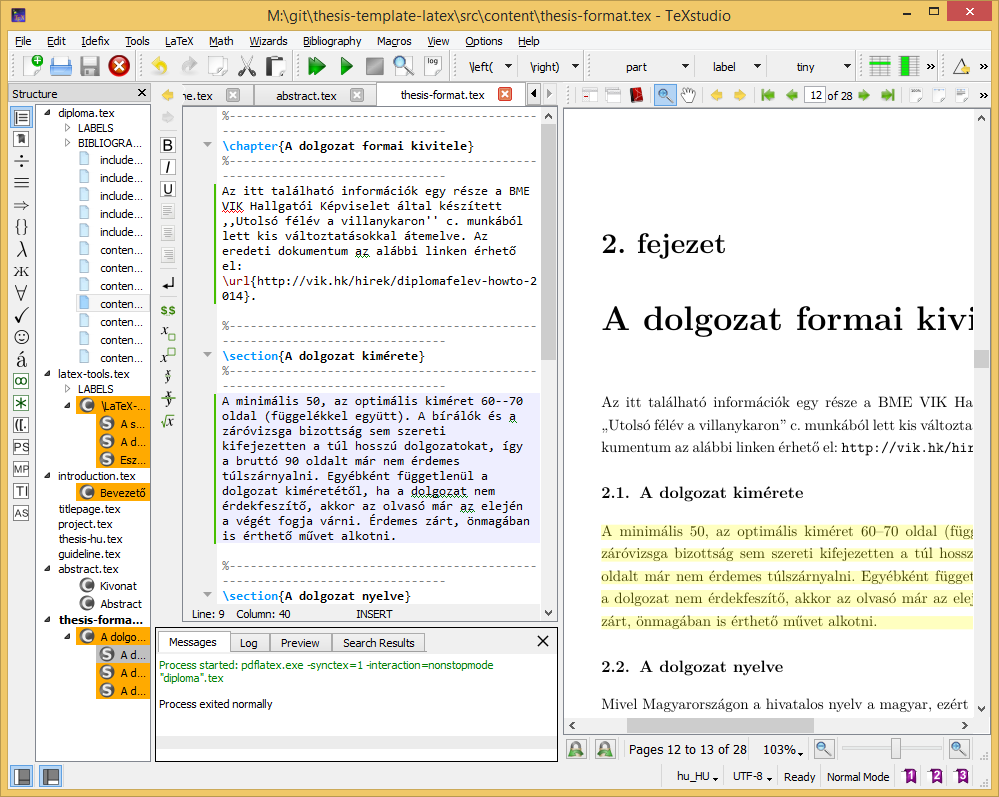
\includegraphics[width=150mm, keepaspectratio]{figures/TeXstudio.png}
\caption{A TeXstudio \LaTeX-szerkesztő.}
\label{fig:TeXstudio}
\end{figure}

A TeXstudio telepítése után érdemes még letölteni a magyar nyelvű helyesírásellenőrző-szótárakat hozzá. A TeXstudio az OpenOffice-hoz használatos formátumot tudja kezelni. A TeXstudio beállításainál a \verb+General+ fülön a \verb+Dictionaries+ résznél tudjuk megadni, hogy melyik szótárat használja.

Egy másik használható Windows alapú szerkesztőprogram a LEd\footnote{A LEd hivatalos oldala: \url{http://www.latexeditor.org/}} (LaTeX Editor), a TeXstudio azonban stabilabb, gyorsabb, és jobban használható.

%----------------------------------------------------------------------------
\section{A dokumentum lefordítása Windows alatt}
%----------------------------------------------------------------------------
A TeXstudio és a LEd kizárólag szerkesztőprogram (bár az utóbbiban DVI-nézegető is van), így a dokumentum fordításához szükséges eszközöket nem tartalmazza. Windows alatt alapvetően két lehetőség közül érdemes választani: MiKTeX (\url{http://miktex.org/}) és TeX Live (\url{http://www.tug.org/texlive/}) programcsomag. Az utóbbi működik Mac OS X, GNU/Linux alatt és Unix-származékokon is. A MiKTeX egy alapcsomag telepítése után mindig letölti a használt funkciókhoz szükséges, de lokálisan hiányzó \TeX-csomagokat, míg a TeX Live DVD ISO verzóban férhető hozzá. Ez a dokumentum TeX Live 2008 programcsomag segítségével fordult, amelynek DVD ISO verziója a megadott oldalról letölthető. A sablon lefordításához a disztribúcióban szereplő \verb+magyar.ldf+ fájlt a \verb+http://www.math.bme.hu/latex/+ változatra kell cserélni, vagy az utóbbi változatot be kell másolni a projekt-könyvtárba (ahogy ezt meg is tettük a sablonban) különben anomáliák tapasztalhatók a dokumentumban (pl. az ábra- és táblázat-aláírások formátuma nem a beállított lesz, vagy bizonyos oldalakon megjelenik alapértelmezésben egy fejléc). A TeX Live 2008-at még nem kell külön telepíteni a gépre, elegendő DVD-ről (vagy az ISO fájlból közvetlenül, pl. DaemonTools-szal) használni.

Ha a MiKTeX csomagot használjuk, akkor parancssorból a következő módon tudjuk újrafordítani a teljes dokumentumot:

\begin{lstlisting}[language=bash,frame=single,float=!ht]
$ texify -p thesis.tex
\end{lstlisting}

A \verb+texify+ parancs a MiKTex programcsomag \verb+miktex/bin+ alkönyvtárában található. A parancs gondoskodik arról, hogy a szükséges lépéseket (fordítás, hivatkozások generálása stb.) a megfelelő sorrendben elvégezze. A \verb+-p+ kapcsoló hatására PDF-et generál. A fordítást és az ideiglenes fájlok törlését elvégezhetjük a sablonhoz mellékelt \verb+manual_build.bat+ szkript segítségével is.

A \TeX-eszközöket tartalmazó programcsomag binárisainak elérési útját gyakran be kell állítani a szerkesztőprogramban, például TeXstudio esetén legegyszerűbben az \verb+Options / Configure TeXstudio... / Commands+ menüponttal előhívott dialógusablakban tehetjük ezt meg.

A PDF-\LaTeX~használata esetén a generált dokumentum közvetlenül PDF-formátumban áll rendelkezésre. Amennyiben a PDF-fájl egy PDF-nézőben (pl. Adobe Acrobat Reader vagy Foxit PDF Reader) meg van nyitva, akkor a fájlleírót a PDF-néző program tipikusan lefoglalja. Ilyen esetben a dokumentum újrafordítása hibaüzenettel kilép. Ha bezárjuk és újra megnyitjuk a PDF dokumentumot, akkor pedig a PDF-nézők többsége az első oldalon nyitja meg a dokumentumot, nem a legutóbb olvasott oldalon. Ezzel szemben például az egyszerű és ingyenes \textcolor{blue}{Sumatra PDF} nevű program képes arra, hogy a megnyitott dokumentum megváltozását detektálja, és frissítse a nézetet az aktuális oldal megtartásával.

%----------------------------------------------------------------------------
\section{Eszközök Linuxhoz}
%----------------------------------------------------------------------------
Linux operációs rendszer alatt is rengeteg szerkesztőprogram van, pl. a KDE alapú Kile jól használható. Ez ingyenesen letölthető, vagy éppenséggel az adott Linux-disztribúció eleve tartalmazza, ahogyan a dokumentum fordításához szükséges csomagokat is. Az Ubuntu Linux disztribúciók alatt például legtöbbször a \verb+texlive-*+ csomagok telepítésével használhatók a \LaTeX-eszközök. A jelen sablon fordításához szükséges csomagok (kb. 0,5 GB) az alábbi paranccsal telepíthetők:

\begin{lstlisting}[language=bash,morekeywords={sudo,apt\-get},alsoletter={-},breaklines=true]
$ sudo apt-get install texlive-latex-extra texlive-fonts-extra texlive-fonts-recommended texlive-xetex texlive-science
\end{lstlisting}

Amennyiben egy újabb csomag hozzáadása után hiányzó fájlra utaló hibát kapunk a fordítótól, telepítenünk kell az azt tartalmazó TeX Live csomagot. Ha pl. a \verb+bibentry+ csomagot szeretnénk használni, futtassuk az alábbi parancsot:

\begin{lstlisting}[language=bash,morekeywords={apt\-cache},alsoletter={-},breaklines=true]
$ apt-cache search bibentry
texlive-luatex - TeX Live: LuaTeX packages
\end{lstlisting}

Majd telepítsük fel a megfelelő TeX Live csomagot, jelen esetben a `texlive-lualatex`-et. (Egy LaTeX csomag több TeX Live csomagban is szerepelhet.)

Ha gyakran szerkesztünk más \LaTeX dokumentumokat is, kényelmes és biztos megoldás a teljes TeX Live disztribúció telepítése, ez azonban kb. 4 GB helyet igényel.

\begin{lstlisting}[language=bash,morekeywords={sudo,apt\-get},alsoletter={-},breaklines=true]
sudo apt-get install texlive-full
\end{lstlisting}

%%----------------------------------------------------------------------------
\chapter{A dolgozat formai kivitele}
%----------------------------------------------------------------------------
Az itt található információk egy része a BME VIK Hallgatói Képviselet által készített ,,Utolsó félév a villanykaron'' c. munkából lett kis változtatásokkal átemelve. Az eredeti dokumentum az alábbi linken érhető el: \url{http://vik.hk/hirek/diplomafelev-howto-2015}.

%----------------------------------------------------------------------------
\section{A dolgozat kimérete}
%----------------------------------------------------------------------------
Szakdolgozat esetében minimum 30, 45 körüli ajánlott oldalszám lehet az iránymutató. De mindenképp érdemes rákérdezni a konzulensnél is az elvárásokra, mert tanszékenként változóak lehetnek az elvárások.

Mesterképzésen a Diplomatervezés 1 esetében a beszámoló még inkább az Önálló laboratóriumi beszámolókhoz hasonlít, tanszékenként eltérő formai követelményekkel, -- egy legalább 30 oldal körüli dolgozat az elvárt -- és az elmúlt fél éves munkáról szól. De egyben célszerű, ha ez a végleges diplomaterv alapja is. (A végleges 60-90 oldal körülbelül a hasznos részre nézve)


%----------------------------------------------------------------------------
\section{A dolgozat nyelve}
%----------------------------------------------------------------------------
Mivel Magyarországon a hivatalos nyelv a magyar, ezért alapértelmezésben magyarul kell megírni a dolgozatot. Aki külföldi posztgraduális képzésben akar részt venni, nemzetközi szintű tudományos kutatást szeretne végezni, vagy multinacionális cégnél akar elhelyezkedni, annak célszerű angolul megírnia diplomadolgozatát. Mielőtt a hallgató az angol nyelvű verzió mellett dönt, erősen ajánlott mérlegelni, hogy ez mennyi többletmunkát fog a hallgatónak jelenteni fogalmazás és nyelvhelyesség terén, valamint -- nem utolsó sorban -- hogy ez mennyi többletmunkát fog jelenteni a konzulens illetve bíráló számára. Egy nehezen olvasható, netalán érthetetlen szöveg teher minden játékos számára.

%----------------------------------------------------------------------------
\section{A dokumentum nyomdatechnikai kivitele}
%----------------------------------------------------------------------------
A dolgozatot A4-es fehér lapra nyomtatva, 2,5 centiméteres margóval (+1~cm kötésbeni), 11--12 pontos betűmérettel, talpas betűtípussal és másfeles sorközzel célszerű elkészíteni.

Annak érdekében, hogy a dolgozat külsőleg is igényes munka benyomását keltse, érdemes figyelni az alapvető tipográfiai szabályok betartására~\cite{Jeney}.

%% !TeX spellcheck = hu_HU
% !TeX encoding = UTF-8
% !TeX program = xelatex
%----------------------------------------------------------------------------
\chapter{A \LaTeX-sablon használata}
%----------------------------------------------------------------------------

Ebben a fejezetben röviden, implicit módon bemutatjuk a sablon használatának módját, ami azt jelenti, hogy sablon használata ennek a dokumentumnak a forráskódját tanulmányozva válik teljesen világossá. Amennyiben a szoftver-keretrendszer telepítve van, a sablon alkalmazása és a dolgozat szerkesztése \LaTeX-ben a sablon segítségével tapasztalataink szerint jóval hatékonyabb, mint egy WYSWYG (\emph{What You See is What You Get}) típusú szövegszerkesztő esetén (pl. Microsoft Word, OpenOffice).

%----------------------------------------------------------------------------
\section{Címkék és hivatkozások}
%----------------------------------------------------------------------------
A \LaTeX~dokumentumban címkéket (\verb+\label+) rendelhetünk ábrákhoz, táblázatokhoz, fejezetekhez, listákhoz, képletekhez stb. Ezekre a dokumentum bármely részében hivatkozhatunk, a hivatkozások automatikusan feloldásra kerülnek.

A sablonban makrókat definiáltunk a hivatkozások megkönnyítéséhez. Ennek megfelelően minden ábra (\emph{figure}) címkéje \verb+fig:+ kulcsszóval kezdődik, míg minden táblázat (\emph{table}), képlet (\emph{equation}), fejezet (\emph{section}) és lista (\emph{listing}) rendre a \verb+tab:+, \verb+eq:+, \verb+sec:+ és \verb+lst:+ kulcsszóval kezdődik, és a kulcsszavak után tetszőlegesen választott címke használható. Ha ezt a konvenciót betartjuk, akkor az előbbi objektumok számára rendre a \verb+\figref+, \verb+\tabref+, \verb+\eqref+, \verb+\sectref+ és \verb+\listref+ makrókkal hivatkozhatunk. A makrók paramétere a címke, amelyre hivatkozunk (a kulcsszó nélkül). Az összes említett hivatkozástípus, beleértve az \verb+\url+ kulcsszóval bevezetett web-hivatkozásokat is a  \verb+hyperref+\footnote{Segítségével a dokumentumban megjelenő hivatkozások nem csak dinamikussá válnak, de színezhetők is, bővebbet erről a csomag dokumentációjában találunk. Ez egyúttal egy példa lábjegyzet írására.} csomagnak köszönhetően aktívak a legtöbb PDF-nézegetőben, rájuk kattintva a dokumentum megfelelő oldalára ugrik a PDF-néző vagy a megfelelő linket megnyitja az alapértelmezett böngészővel. A \verb+hyperref+ csomag a kimeneti PDF-dokumentumba könyvjelzőket is készít a tartalomjegyzékből. Ez egy szintén aktív tartalomjegyzék, amelynek elemeire kattintva a nézegető behozza a kiválasztott fejezetet.

%----------------------------------------------------------------------------
\section{Ábrák és táblázatok}
%----------------------------------------------------------------------------
Használjunk vektorgrafikus ábrákat, ha van rá módunk. PDFLaTeX használata esetén PDF formátumú ábrákat lehet beilleszteni könnyen, az EPS (PostScript) vektorgrafikus képformátum beillesztését a PDFLaTeX közvetlenül nem támogatja (de lehet konvertálni, lásd később). Ha vektorgrafikus formában nem áll rendelkezésünkre az ábra, akkor a  veszteségmentes PNG, valamint a veszteséges JPEG formátumban érdemes elmenteni.  Figyeljünk arra, hogy ilyenkor a képek felbontása elég nagy legyen ahhoz, hogy nyomtatásban is megfelelő minőséget nyújtson (legalább 300 dpi javasolt). A dokumentumban felhasznált képfájlokat a dokumentum forrása mellett érdemes tartani, archiválni, mivel ezek hiányában a dokumentum nem fordul újra. Ha lehet, a vektorgrafikus képeket vektorgrafikus formátumban is érdemes elmenteni az újrafelhasználhatóság (az átszerkeszthetőség) érdekében.

Kapcsolási rajzok legtöbbször kimásolhatók egy vektorgrafikus programba (pl. CorelDraw) és onnan nagyobb felbontással raszterizálva kimenthatők PNG formátumban. Ugyanakkor kiváló ábrák készíthetők Microsoft Visio vagy hasonló program használatával is: Visio-ból az ábrák közvetlenül PDF-be is menthetők.

Lehetőségeink Matlab ábrák esetén:
\begin{itemize}
	\item Képernyőlopás (\emph{screenshot}) is elfogadható minőségű lehet a dokumentumban, de általában jobb felbontást is el lehet érni más módszerrel.
	\item A Matlab ábrát a \verb+File/Save As+ opcióval lementhetjük PNG formátumban (ugyanaz itt is érvényes, mint korábban, ezért nem javasoljuk).
	\item A Matlab ábrát az \verb+Edit/Copy figure+ opcióval kimásolhatjuk egy vektorgrafikus programba is és onnan nagyobb felbontással raszterizálva kimenthatjük PNG formátumban (nem javasolt).
	\item Javasolt megoldás: az ábrát a \verb+File/Save As+ opcióval EPS \emph{vektorgrafikus} formátumban elmentjük, PDF-be konvertálva beillesztjük a dolgozatba.
\end{itemize}
Az EPS kép az \verb+epstopdf+ programmal\footnote{a korábban említett \LaTeX-disztribúciókban megtalálható} konvertálható PDF formátumba. Célszerű egy batch-fájlt készíteni az összes EPS ábra lefordítására az alábbi módon (ez Windows alatt működik).
\begin{lstlisting}[language=]
@echo off
for %%j in (*.eps) do (
  echo converting file "%%j"
  epstopdf "%%j"
)
echo done .
\end{lstlisting}

Egy ilyen parancsfájlt (\verb+convert.cmd+) elhelyeztük a sablon \verb+figures\eps+ könyvtárába, így a felhasználónak csak annyi a dolga, hogy a \verb+figures\eps+ könyvtárba kimenti az EPS formátumú vektorgrafikus képet, majd lefuttatja a \verb+convert.cmd+ parancsfájlt, ami PDF-be konvertálja az EPS fájlt.

Ezek után a PDF-ábrát ugyanúgy lehet a dokumentumba beilleszteni, mint a PNG-t vagy a JPEG-et. A megoldás előnye, hogy a lefordított dokumentumban is vektorgrafikusan tárolódik az ábra, így a mérete jóval kisebb, mintha raszterizáltuk volna beillesztés előtt. Ez a módszer minden -- az EPS formátumot ismerő -- vektorgrafikus program (pl. CorelDraw) esetén is használható.

A képek beillesztésére \az+\refstruc{sec:LatexTools}ben mutattunk be példát (\refstruc{fig:TeXstudio}). Az előző mondatban egyúttal az automatikusan feloldódó ábrahivatkozásra is láthatunk példát. Több képfájlt is beilleszthetünk egyetlen ábrába. Az egyes képek közötti horizontális és vertikális margót metrikusan szabályozhatjuk (\refstruc{fig:HVSpaces}). Az ábrák elhelyezését számtalan tipográfiai szabály egyidejű teljesítésével a fordító maga végzi, a dokumentum írója csak preferenciáit jelezheti a fordító felé (olykor ez bosszúságot is okozhat, ilyenkor pl. a kép méretével lehet játszani).

\begin{figure}[!ht]
	\centering
	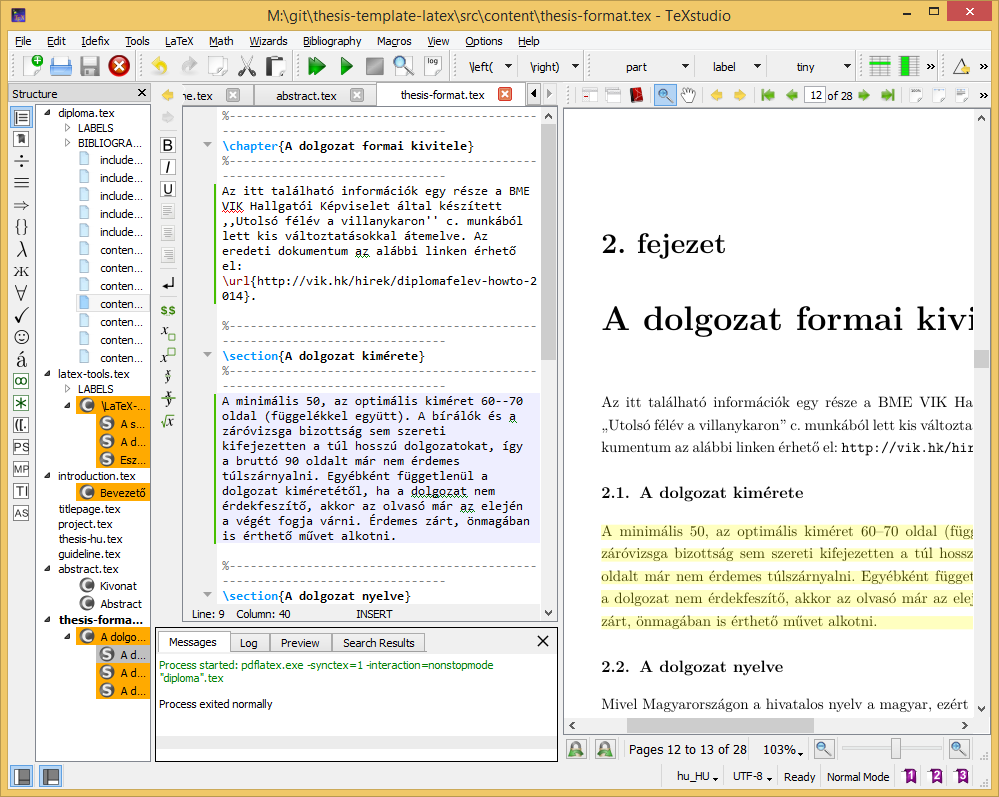
\includegraphics[width=67mm, keepaspectratio]{figures/TeXstudio.png}\hspace{1cm}
	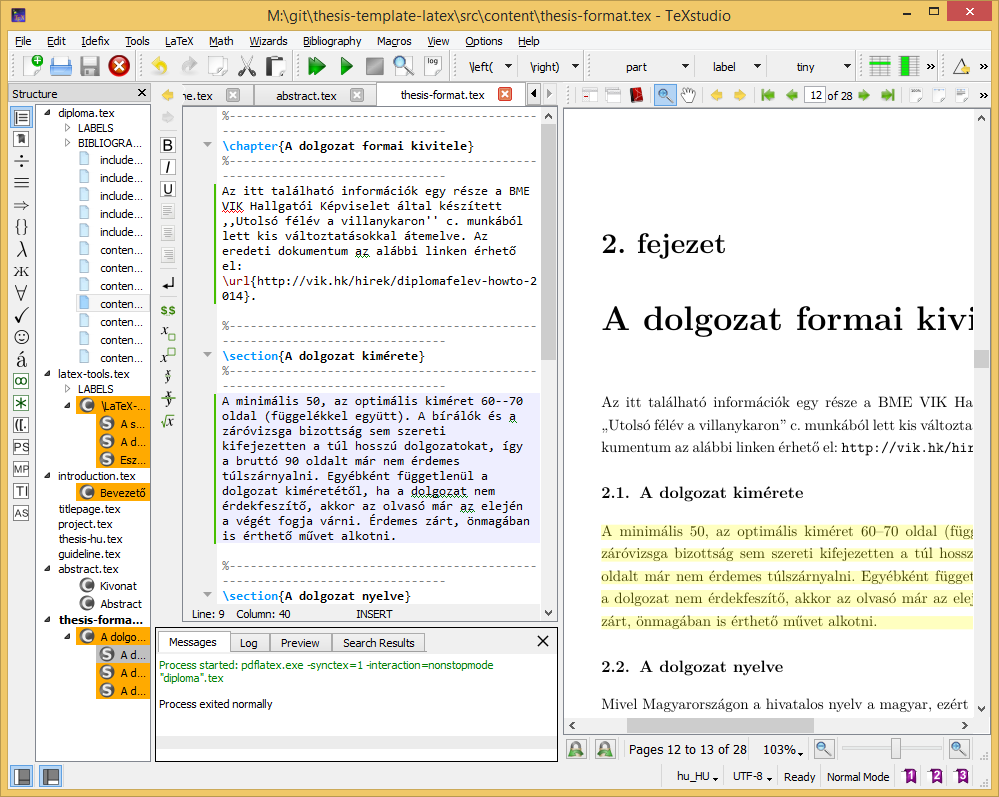
\includegraphics[width=67mm, keepaspectratio]{figures/TeXstudio.png}\\\vspace{5mm}
	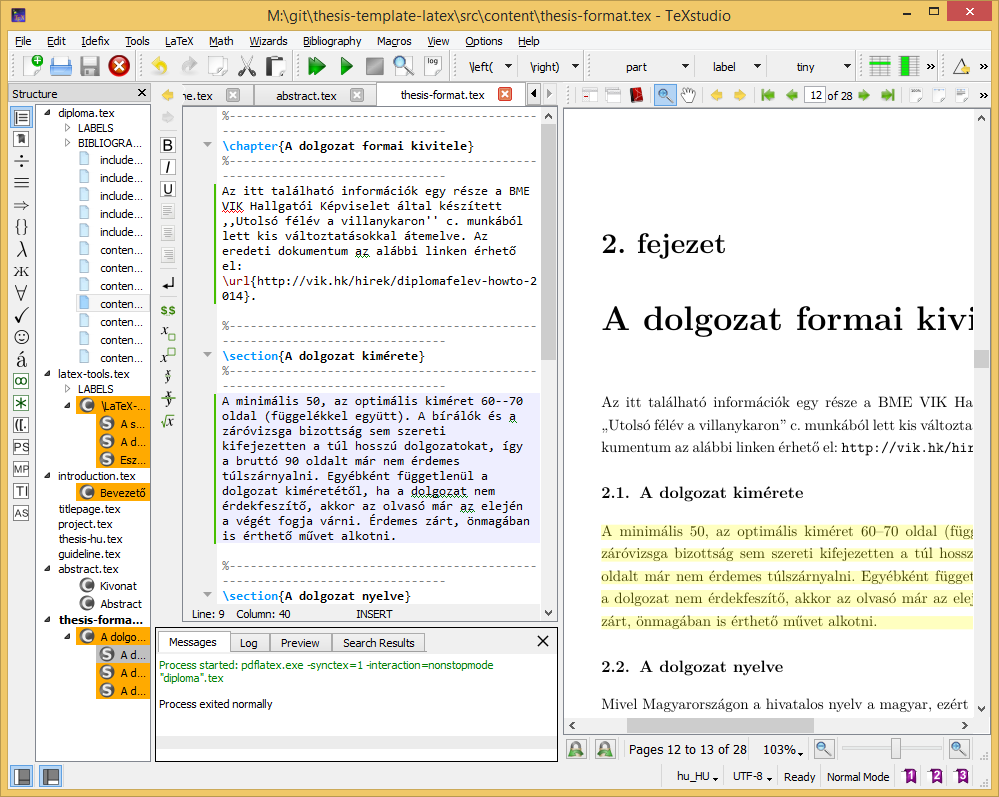
\includegraphics[width=67mm, keepaspectratio]{figures/TeXstudio.png}\hspace{1cm}
	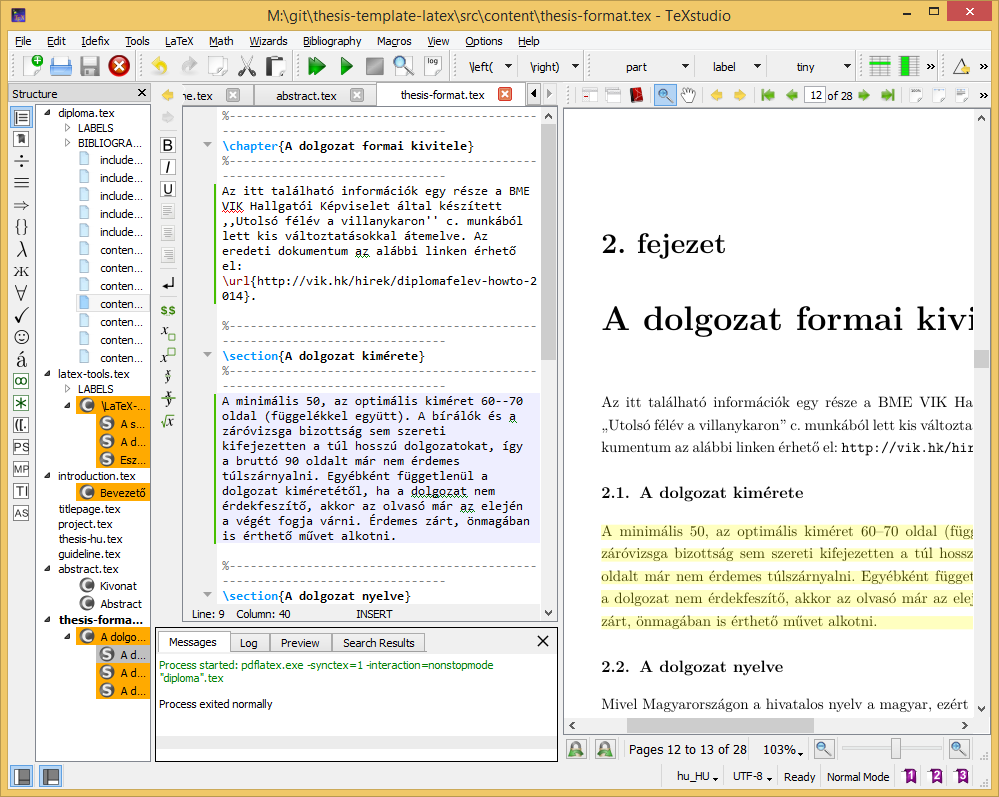
\includegraphics[width=67mm, keepaspectratio]{figures/TeXstudio.png}
	\caption{Több képfájl beillesztése esetén térközöket is érdemes használni.}
	\label{fig:HVSpaces}
\end{figure}

A táblázatok használatára \aref{tab:TabularExample}~táblázat mutat példát. A táblázatok formázásához hasznos tanácsokat találunk a \verb+booktabs+ csomag dokumentációjában.

\begin{table}[ht]
	\footnotesize
	\centering
	\begin{tabular}{ l c c }
		\toprule
		Órajel & Frekvencia & Cél pin \\
		\midrule
		CLKA & 100 MHz & FPGA CLK0\\
		CLKB & 48 MHz  & FPGA CLK1\\
		CLKC & 20 MHz  & Processzor\\
		CLKD & 25 MHz  & Ethernet chip \\
		CLKE & 72 MHz  & FPGA CLK2\\
		XBUF & 20 MHz  & FPGA CLK3\\
		\bottomrule
	\end{tabular}
	\caption{Az órajel-generátor chip órajel-kimenetei.}
	\label{tab:TabularExample}
\end{table}


%----------------------------------------------------------------------------
\section{Felsorolások és listák}
%----------------------------------------------------------------------------
Számozatlan felsorolásra mutat példát a jelenlegi bekezdés:
\begin{itemize}
	\item \emph{első bajusz:} ide lehetne írni az első elem kifejését,
	\item \emph{második bajusz:} ide lehetne írni a második elem kifejését,
	\item \emph{ez meg egy szakáll:} ide lehetne írni a harmadik elem kifejését.
\end{itemize}

Számozott felsorolást is készíthetünk az alábbi módon:
\begin{enumerate}
	\item \emph{első bajusz:} ide lehetne írni az első elem kifejését, és ez a kifejtés így néz ki, ha több sorosra sikeredik,
	\item \emph{második bajusz:} ide lehetne írni a második elem kifejését,
	\item \emph{ez meg egy szakáll:} ide lehetne írni a harmadik elem kifejését.
\end{enumerate}
A felsorolásokban sorok végén vessző, az utolsó sor végén pedig pont a szokásos írásjel. Ez alól kivételt képezhet, ha az egyes elemek több teljes mondatot tartalmaznak.

Listákban a dolgozat szövegétől elkülönítendő kódrészleteket, programsorokat, pszeudo-kódokat jeleníthetünk meg (\ref{lst:Example}.~kódrészlet).
\begin{lstlisting}[language=tex,caption=A fenti számozott felsorolás \LaTeX-forráskódja,label=lst:Example]
\begin{enumerate}
	\item \emph{els(*@ő@*) bajusz:} ide lehetne írni az els(*@ő@*) elem kifejését,
	és ez a kifejtés így néz ki, ha több sorosra sikeredik,
	\item \emph{második bajusz:} ide lehetne írni a második elem kifejését,
	\item \emph{ez meg egy szakáll:} ide lehetne írni a harmadik elem kifejését.
\end{enumerate}
\end{lstlisting}
A lista keretét, háttérszínét, egész stílusát megválaszthatjuk. Ráadásul különféle programnyelveket és a nyelveken belül kulcsszavakat is definiálhatunk, ha szükséges. Erről bővebbet a \verb+listings+ csomag hivatalos leírásában találhatunk.

%----------------------------------------------------------------------------
\section{Képletek}
%----------------------------------------------------------------------------
Ha egy formula nem túlságosan hosszú, és nem akarjuk hivatkozni a szövegből, mint például a $e^{i\pi}+1=0$ képlet, \emph{szövegközi képletként} szokás leírni. Csak, hogy másik példát is lássunk, az $U_i=-d\Phi/dt$ Faraday-törvény a $\rot E=-\frac{dB}{dt}$ differenciális alakban adott Maxwell-egyenlet felületre vett integráljából vezethető le. Látható, hogy a \LaTeX-fordító a sorközöket betartja, így a szöveg szedése esztétikus marad szövegközi képletek használata esetén is.

Képletek esetén az általános konvenció, hogy a kisbetűk skalárt, a kis félkövér betűk ($\mathbf{v}$) oszlopvektort -- és ennek megfelelően $\mathbf{v}^T$ sorvektort -- a kapitális félkövér betűk ($\mathbf{V}$) mátrixot jelölnek. Ha ettől el szeretnénk térni, akkor az alkalmazni kívánt jelölésmódot célszerű külön alfejezetben definiálni. Ennek megfelelően, amennyiben $\mathbf{y}$ jelöli a mérések vektorát, $\mathbf{\vartheta}$ a paraméterek vektorát és $\hat{\mathbf{y}}=\mathbf{X}\vartheta$ a paraméterekben lineáris modellt, akkor a \emph{Least-Squares} értelemben optimális paraméterbecslő $\hat{\mathbf{\vartheta}}_{LS}=(\mathbf{X}^T\mathbf{X})^{-1}\mathbf{X}^T\mathbf{y}$ lesz.

Emellett kiemelt, sorszámozott képleteket is megadhatunk, ennél az \verb+equation+ és a \verb+eqnarray+ környezetek helyett a korszerűbb \verb+align+ környezet alkalmazását javasoljuk (több okból, különféle problémák elkerülése végett, amelyekre most nem térünk ki). Tehát
\begin{align}
\dot{\mathbf{x}}&=\mathbf{A}\mathbf{x}+\mathbf{B}\mathbf{u},\\
\mathbf{y}&=\mathbf{C}\mathbf{x},
\end{align}
ahol $\mathbf{x}$ az állapotvektor, $\mathbf{y}$ a mérések vektora és $\mathbf{A}$, $\mathbf{B}$ és $\mathbf{C}$ a rendszert leíró paramétermátrixok. Figyeljük meg, hogy a két egyenletben az egyenlőségjelek egymáshoz igazítva jelennek meg, mivel a mindkettőt az \& karakter előzi meg a kódban. Lehetőség van számozatlan kiemelt képlet használatára is, például
\begin{align}
\dot{\mathbf{x}}&=\mathbf{A}\mathbf{x}+\mathbf{B}\mathbf{u},\nonumber\\
\mathbf{y}&=\mathbf{C}\mathbf{x}\nonumber.
\end{align}
Mátrixok felírására az $\mathbf{A}\mathbf{x}=\mathbf{b}$ inhomogén lineáris egyenlet részletes kifejtésével mutatunk példát:
\begin{align}
\begin{bmatrix}
a_{11} & a_{12} & \dots & a_{1n}\\
a_{21} & a_{22} & \dots & a_{2n}\\
\vdots & \vdots & \ddots & \vdots\\
a_{m1} & a_{m2} & \dots & a_{mn}
\end{bmatrix}
\begin{pmatrix}x_1\\x_2\\\vdots\\x_n\end{pmatrix}=
\begin{pmatrix}b_1\\b_2\\\vdots\\b_m\end{pmatrix}.
\end{align}
A \verb+\frac+ utasítás hatékonyságát egy általános másodfokú tag átviteli függvényén keresztül mutatjuk be, azaz
\begin{align}
W(s)=\frac{A}{1+2T\xi s+s^2T^2}.
\end{align}
A matematikai mód minden szimbólumának és képességének a bemutatására természetesen itt nincs lehetőség, de gyors referenciaként hatékonyan használhatók a következő linkek:\\
\indent\url{http://www.artofproblemsolving.com/LaTeX/AoPS_L_GuideSym.php},\\
\indent\url{http://www.ctan.org/tex-archive/info/symbols/comprehensive/symbols-a4.pdf},\\
\indent\url{ftp://ftp.ams.org/pub/tex/doc/amsmath/short-math-guide.pdf}.\\
Ez pedig itt egy magyarázat, hogy miért érdemes \verb+align+ környezetet használni:\\
\indent\url{http://texblog.net/latex-archive/maths/eqnarray-align-environment/}.

%----------------------------------------------------------------------------
\section{Irodalmi hivatkozások}
\label{sec:HowtoReference}
%----------------------------------------------------------------------------
Egy \LaTeX~dokumentumban az irodalmi hivatkozások definíciójának két módja van. Az egyik a \verb+\thebibliograhy+ környezet használata a dokumentum végén, az \verb+\end{document}+ lezárás előtt.
\begin{lstlisting}[language=tex]
\begin{thebibliography}{9}

\bibitem{Lamport94} Leslie Lamport, \emph{\LaTeX: A Document Preparation System}.
Addison Wesley, Massachusetts, 2nd Edition, 1994.

\end{thebibliography}
\end{lstlisting}

Ezek után a dokumentumban a \verb+\cite{Lamport94}+ utasítással hivatkozhatunk a forrásra. A fenti megadás viszonylag kötetlen, a szerző maga formázza az irodalomjegyzéket (ami gyakran inkonzisztens eredményhez vezet).

Egy sokkal professzionálisabb módszer a BiB\TeX{} használata, ezért ez a sablon is ezt támogatja. Ebben az esetben egy külön szöveges adatbázisban definiáljuk a forrásmunkákat, és egy külön stílusfájl határozza meg az irodalomjegyzék kinézetét. Ez, összhangban azzal, hogy külön formátumkonvenció határozza meg a folyóirat-, a könyv-, a konferenciacikk- stb. hivatkozások kinézetét az irodalomjegyzékben (a sablon használata esetén ezzel nem is kell foglalkoznia a hallgatónak, de az eredményt célszerű ellenőrizni). felhasznált hivatkozások adatbázisa egy \verb+.bib+ kiterjesztésű szöveges fájl, amelynek szerkezetét a \Aref{lst:Bibtex} kódrészlet demonstrálja. A forrásmunkák bevitelekor a sor végi vesszők külön figyelmet igényelnek, mert hiányuk a BiB\TeX-fordító hibaüzenetét eredményezi. A forrásmunkákat típus szerinti kulcsszó vezeti be (\verb+@book+ könyv, \verb+@inproceedings+ konferenciakiadványban megjelent cikk, \verb+@article+ folyóiratban megjelent cikk, \verb+@techreport+ valamelyik egyetem gondozásában megjelent műszaki tanulmány, \verb+@manual+ műszaki dokumentáció esetén stb.). Nemcsak a megjelenés stílusa, de a kötelezően megadandó mezők is típusról-típusra változnak. Egy jól használható referencia a \url{http://en.wikipedia.org/wiki/BibTeX} oldalon található.

\begin{lstlisting}[caption=Példa szöveges irodalomjegyzék-adatbázisra Bib\TeX{} használata esetén.,label=lst:Bibtex]
@book{Wettl04,
  author    = {Ferenc Wettl and Gyula Mayer and Péter Szabó},
  publisher = {Panem Könyvkiadó},
  title     = {\LaTeX~kézikönyv},
  year      = {2004},
}

@article{Candy86,
  author       = {James C. Candy},
  journaltitle = {{IEEE} Trans.\ on Communications},
  month        = {01},
  note         = {\doi{10.1109/TCOM.1986.1096432}},
  number       = {1},
  pages        = {72--76},
  title        = {Decimation for Sigma Delta Modulation},
  volume       = {34},
  year         = {1986},
}

@inproceedings{Lee87,
  author    = {Wai L. Lee and Charles G. Sodini},
  booktitle = {Proc.\ of the IEEE International Symposium on Circuits and Systems},
  location  = {Philadelphia, PA, USA},
  month     = {05~4--7},
  pages     = {459--462},
  title     = {A Topology for Higher Order Interpolative Coders},
  vol       = {2},
  year      = {1987},
}

@thesis{KissPhD,
  author      = {Peter Kiss},
  institution = {Technical University of Timi\c{s}oara, Romania},
  month       = {04},
  title       = {Adaptive Digital Compensation of Analog Circuit Imperfections for Cascaded Delta-Sigma Analog-to-Digital Converters},
  type        = {phdthesis},
  year        = {2000},
}

@manual{Schreier00,
  author       = {Richard Schreier},
  month        = {01},
  note         = {\url{http://www.mathworks.com/matlabcentral/fileexchange/}},
  organization = {Oregon State University},
  title        = {The Delta-Sigma Toolbox v5.2},
  year         = {2000},
}

@misc{DipPortal,
  author       = {{Budapesti Műszaki és Gazdaságtudományi Egyetem Villamosmérnöki és Informatikai Kar}},
  howpublished = {\url{http://diplomaterv.vik.bme.hu/}},
  title        = {Diplomaterv portál (2011. február 26.)},
}

@incollection{Mkrtychev:1997,
  author    = {Mkrtychev, Alexey},
  booktitle = {Logical Foundations of Computer Science},
  doi       = {10.1007/3-540-63045-7_27},
  editor    = {Adian, Sergei and Nerode, Anil},
  isbn      = {978-3-540-63045-6},
  pages     = {266-275},
  publisher = {Springer Berlin Heidelberg},
  series    = {Lecture Notes in Computer Science},
  title     = {Models for the logic of proofs},
  url       = {http://dx.doi.org/10.1007/3-540-63045-7_27},
  volume    = {1234},
  year      = {1997},
}
\end{lstlisting}

A stílusfájl egy \verb+.sty+ kiterjesztésű fájl, de ezzel lényegében nem kell foglalkozni, mert vannak beépített stílusok, amelyek jól használhatók. Ez a sablon a BiB\TeX-et használja, a hozzá tartozó adatbázisfájl a \verb+mybib.bib+ fájl. Megfigyelhető, hogy az irodalomjegyzéket a dokumentum végére (a \verb+\end{document}+ utasítás elé) beillesztett \verb+\bibliography{mybib}+ utasítással hozhatjuk létre, a stílusát pedig ugyanitt a  \verb+\bibliographystyle{plain}+ utasítással adhatjuk meg. Ebben az esetben a \verb+plain+ előre definiált stílust használjuk (a sablonban is ezt állítottuk be). A \verb+plain+ stíluson kívül természetesen számtalan más előre definiált stílus is létezik. Mivel a \verb+.bib+ adatbázisban ezeket megadtuk, a BiB\TeX-fordító is meg tudja különböztetni a szerzőt a címtől és a kiadótól, és ez alapján automatikusan generálódik az irodalomjegyzék a stílusfájl által meghatározott stílusban.

Az egyes forrásmunkákra a szövegből továbbra is a \verb+\cite+ paranccsal tudunk hivatkozni, így \aref{lst:Bibtex}.~kódrészlet esetén a hivatkozások rendre \verb+\cite{Wettl04}+, \verb+\cite{Candy86}+, \verb+\cite{Lee87}+, \verb+\cite{KissPhD}+, \verb+\cite{Schreirer00}+,
\verb+\cite{Mkrtychev:1997}+ és \verb+\cite{DipPortal}+. Az egyes forrásmunkák sorszáma az irodalomjegyzék bővítésekor változhat. Amennyiben az aktuális számhoz illeszkedő névelőt szeretnénk használni, használjuk az \verb+\acite{}+ parancsot.

Az irodalomjegyzékben alapértelmezésben csak azok a forrásmunkák jelennek meg, amelyekre található hivatkozás a szövegben, és ez így alapvetően helyes is, hiszen olyan forrásmunkákat nem illik az irodalomjegyzékbe írni, amelyekre nincs hivatkozás.

Mivel a fordítási folyamat során több lépésben oldódnak fel a szimbólumok, ezért gyakran többször is le kell fordítani a dokumentumot. Ilyenkor ez első 1-2 fordítás esetleg szimbólum-feloldásra vonatkozó figyelmeztető üzenettel zárul. Ha hibaüzenettel zárul bármelyik fordítás, akkor nincs értelme megismételni, hanem a hibát kell megkeresni. A \verb+.bib+ fájl megváltoztatáskor sokszor nincs hatása a változtatásnak azonnal, mivel nem mindig fut újra a BibTeX fordító. Ezért célszerű a változtatás után azt manuálisan is lefuttatni (TeXstudio esetén \verb+Tools/Bibliography+).

Hogy a szövegbe ágyazott hivatkozások kinézetét demonstráljuk, itt most sorban meghivatkozzuk a \cite{Wettl04}, \cite{Candy86}, \cite{Lee87}, \cite{KissPhD}, \cite{Schreier00} és \acite{Mkrtychev:1997}\footnote{Informatikai témában gyakran hivatkozunk cikkeket a Springer LNCS valamely kötetéből, ez a hivatkozás erre mutat egy helyes példát.} forrásmunkát, valamint \acite{DipPortal} weboldalt.

Megjegyzendő, hogy az ékezetes magyar betűket is tartalmazó \verb+.bib+ fájl az \verb+inputenc+ csomaggal betöltött \verb+latin2+ betűkészlet miatt fordítható. Ugyanez a \verb+.bib+ fájl hibaüzenettel fordul egy olyan dokumentumban, ami nem tartalmazza a \verb+\usepackage[latin2]{inputenc}+ sort. Speciális igény esetén az irodalmi adatbázis általánosabb érvényűvé tehető, ha az ékezetes betűket speciális latex karakterekkel helyettesítjük a \verb+.bib+ fájlban, pl. á helyett \verb+\'{a}+-t vagy ő helyett \verb+\H{o}+-t írunk.

Irodalomhivatkozásokat célszerű először olyan szolgáltatásokban keresni, ahol jó minőségű bejegyzések találhatók (pl. ACM Digital Library,\footnote{\url{https://dl.acm.org/}} DBLP,\footnote{\url{http://dblp.uni-trier.de/}} IEEE Xplore,\footnote{\url{http://ieeexplore.ieee.org/}} SpringerLink\footnote{\url{https://link.springer.com/}}) és csak ezek után használni kevésbé válogatott forrásokat (pl. Google Scholar\footnote{\url{http://scholar.google.com/}}). A jó minőségű bejegyzéseket is érdemes megfelelően tisztítani.\footnote{\url{https://github.com/FTSRG/cheat-sheets/wiki/BibTeX-Fixing-entries-from-common-sources}} A sablon angol nyelvű változatában használt \texttt{plainnat} beállítás egyik sajátossága, hogy a cikkhez generált hivatkozás a cikk DOI-ját és URL-jét is tartalmazza, ami gyakran duplikátumhoz vezet -- érdemes tehát a DOI-kat tartalmazó URL mezőket törölni. 

%----------------------------------------------------------------------------
\section{A dolgozat szerkezete és a forrásfájlok}
%----------------------------------------------------------------------------
A diplomatervsablonban a TeX fájlok két alkönyvtárban helyezkednek el. Az \verb+include+ könyvtárban azok szerepelnek, amiket tipikusan nem kell szerkesztenünk, ezek a sablon részei (pl. címoldal). A \verb+content+ alkönyvtárban pedig a saját munkánkat helyezhetjük el. Itt érdemes az egyes fejezeteket külön \TeX{} állományokba rakni.

A diplomatervsablon (a kari irányelvek szerint) az alábbi fő fejezetekből áll:
\begin{enumerate}
	\item 1 oldalas \emph{tájékoztató} a szakdolgozat/diplomaterv szerkezetéről (\verb+include/guideline.tex+), ami a végső dolgozatból törlendő,
	\item \emph{feladatkiírás} (\verb+include/project.tex+), a dolgozat nyomtatott verzójában ennek a helyére kerül a tanszék által kiadott, a tanszékvezető által aláírt feladatkiírás, a dolgozat elektronikus verziójába pedig a feladatkiírás egyáltalán ne kerüljön bele, azt külön tölti fel a tanszék a diplomaterv-honlapra,
	\item \emph{címoldal} (\verb+include/titlepage.tex+),
	\item \emph{tartalomjegyzék} (\verb+thesis.tex+),
	\item a diplomatervező \emph{nyilatkozat}a az önálló munkáról (\verb+include/declaration.tex+),
	\item 1-2 oldalas tartalmi \emph{összefoglaló} magyarul és angolul, illetve elkészíthető még további nyelveken is (\verb+content/abstract.tex+),
	\item \emph{bevezetés}: a feladat értelmezése, a tervezés célja, a feladat indokoltsága, a diplomaterv felépítésének rövid összefoglalása (\verb+content/introduction.tex+),
	\item sorszámmal ellátott \emph{fejezetek}: a feladatkiírás pontosítása és részletes elemzése, előzmények (irodalomkutatás, hasonló alkotások), az ezekből levonható következtetések, a tervezés részletes leírása, a döntési lehetőségek értékelése és a választott megoldások indoklása, a megtervezett műszaki alkotás értékelése, kritikai elemzése, továbbfejlesztési lehetőségek,
	\item esetleges \emph{köszönetnyilvánítás}ok (\verb+content/acknowledgement.tex+),
	\item részletes és pontos \emph{irodalomjegyzék} (ez a sablon esetében automatikusan generálódik a \verb+thesis.tex+ fájlban elhelyezett \verb+\bibliography+ utasítás hatására, \az+\refstruc{sec:HowtoReference}ban leírtak szerint),
	\item \emph{függelékek} (\verb+content/appendices.tex+).
\end{enumerate}

A sablonban a fejezetek a \verb+thesis.tex+ fájlba vannak beillesztve \verb+\include+ utasítások segítségével. Lehetőség van arra, hogy csak az éppen szerkesztés alatt álló \verb+.tex+ fájlt fordítsuk le, ezzel lerövidítve a fordítási folyamatot. Ezt a lehetőséget az alábbi kódrészlet biztosítja a \verb+thesis.tex+ fájlban.
\begin{lstlisting}
\includeonly{
	guideline,%
	project,%
	titlepage,%
	declaration,%
	abstract,%
	introduction,%
	chapter1,%
	chapter2,%
	chapter3,%
	acknowledgement,%
	appendices,%
}
\end{lstlisting}

Ha az alábbi kódrészletben az egyes sorokat a \verb+%+ szimbólummal kikommentezzük, akkor a megfelelő \verb+.tex+ fájl nem fordul le. Az oldalszámok és a tartalomjegyék természetesen csak akkor billennek helyre, ha a teljes dokumentumot lefordítjuk.

%----------------------------------------------------------------------------
\newpage
\section{Alapadatok megadása}
%----------------------------------------------------------------------------
A diplomaterv alapadatait (cím, szerző, konzulens, konzulens titulusa) a \verb+thesis.tex+ fájlban lehet megadni.

%----------------------------------------------------------------------------
\section{Új fejezet írása}
%----------------------------------------------------------------------------
A főfejezetek külön \verb+content+ könyvtárban foglalnak helyet. A sablonhoz 3 fejezet készült. További főfejezeteket úgy hozhatunk létre, ha új \TeX~fájlt készítünk a fejezet számára, és a \verb+thesis.tex+ fájlban, a \verb+\include+ és \verb+\includeonly+ utasítások argumentumába felvesszük az új \verb+.tex+ fájl nevét.


%----------------------------------------------------------------------------
\section{Definíciók, tételek, példák}
%----------------------------------------------------------------------------

\begin{definition}[Fluxuskondenzátor térerőssége]
Lorem ipsum dolor sit amet, consectetur adipiscing elit, sed do eiusmod tempor incididunt ut labore et dolore magna aliqua. Ut enim ad minim veniam, quis nostrud exercitation ullamco laboris nisi ut aliquip ex ea commodo consequat.
\end{definition}

\begin{example}
Példa egy példára. Duis aute irure dolor in reprehenderit in voluptate velit esse cillum dolore eu fugiat nulla pariatur. Excepteur sint occaecat cupidatat non proident, sunt in culpa qui officia deserunt mollit anim id est laborum.
\end{example}

\begin{theorem}[Kovács tétele]
Duis aute irure dolor in reprehenderit in voluptate velit esse cillum dolore eu fugiat nulla pariatur. Excepteur sint occaecat cupidatat non proident, sunt in culpa qui officia deserunt mollit anim id est laborum.
\end{theorem}

%----------------------------------------------------------------------------   
\chapter{\bevezetes}
%---------------------------------------------------------------------------- 
A hagyományos VoIP (Voice Over IP) hálózatok általában három részből állnak.
Az első rész, ami egyértelmű a kliensek, akik a hívásokat kezdeményezik és 
fogadják őket. A második maga a SIP (Session Initiation Protocol) szerver, aminek
az a dolga, hogy a kliensek által kapott SIP üzeneteket feldolgozza és ezek alapján
megfelelően állítsa be a harmadik elemet, ami egy RTP (Real-time Transport Protocol) 
proxy. Erre az proxyra azért van szükség, hogy irányítani lehessen az áthaladó 
forgalmat. De ezen felül még rengeteg más funkcióval is rendelkezik egy ilyen
proxy. Az alábbi ábrán látható egy ilyen rendszer egyszerűsített rajza.

\begin{figure}[!ht]
	\centering
	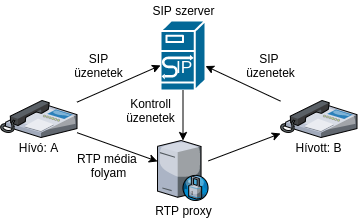
\includegraphics[width=0.5\textwidth, keepaspectratio]{figures/traditional_voip.png}
	\caption{Hagyományos VoIP hálózat}
	\label{fig:HVSpaces}
\end{figure}

Az ábrán egy általános hívásfelépítés látszik, ahol \textbf{A} hívja \textbf{B}-t. 
Ehhez, viszont SIP üzenetekben közölniük kell a SIP szerverrel, hogy ki milyen 
médiaformátumokat fogad el, melyik porton szeretnének kommunikálni a másikkal és 
hasonló információkat. A későbbiekben az összes ilyen protokoll kifejtésre fog
kerülni, hogy könnyebben látható legyen melyikre miért van szükség. Ha a SIP szerver
az összes üzenetet megkapta ahhoz, hogy létre tudjon hozni egy hívást, akkor az 
RTP proxynak megmondja, hogy hozzon létre egy hívást. Ha sikeresen létrejött a 
hívás, akkor kinyit két-két portot a hívásban résztvevő feleknek, amikre érkezhet
az adatfolyam. Azért nyit ki kettő portot kliensenként, mert az egyiken RTP 
csomagokat fog kezelni, míg a másikon RTCP (Real-time Transport Control Protocol) 
csomagokat. Mindezek mellett képes formátum konverziót is végrehajtani. Így ha 
a hívásban lévő két fél nem rendelkezik közös kódolási technikával, akkor is tudnak 
beszélgetni, mert az RTP proxy átfordítja mindkét félnek olyan kódolásra, amit 
képesek használni.

Ezzel a felépítéssel az a probléma, hogy az RTP proxy nem tud végtelen mennyiségű
hívást kezelni port hiányában vagy erőforrás hiány miatt. Így muszáj több példányt
telepíteni a hálózatba, ami jelentősen megbonyolítja a rendszer 
karbantarthatóságát és új problémákat idéz elő. Problémák, amiket ki szeretnék 
küszöbölni a munkám során:

\begin{itemize}
	\item \textbf{Skálázhatóság}: A fő kérdés az, hogy mire történjen a skálázás. 
	\begin{itemize}
		\item Ha nagyon sok a hívás, amik nem igényelnek nagy erőforrást, akkor
		kifuthat az RTP proxy a rendelkezésre álló portokból.
		\item Ha túl sok transzkódolást kell használni, akkor könnyen elfogyhatnak
		a rendelkezésre álló hardveres erőforrások.
		\item A skálázásnak ezenfelül automatikusan kellene működnie. 
	\end{itemize}
	\item \textbf{Rugalmasság}: Mi történik, akkor, ha az egyik RTP proxy szerver
	valamilyen oknál fogva nem üzemel tovább? Ilyenkor is valahogyan kezelni 
	kell a meglévő hívásokat és újakat is kell tudni létrehozni. Erre már van 
	megoldás, ahol egy Redis adatbázissal összetudjuk kötni a példányainkat. 
	Viszont ennek jelenleg van egy olyan hátránya, hogy csak manuálisan lehet 
	új példányt hozzácsatolni ehhez az adatbázishoz, ami rengeteg plusz munkát 
	jelent a nem elhanyagolható mértékű hibázási lehetőség mellett.
	\item \textbf{Automatizálás}: Hogyan lehet a lehető legkevesebb 
	karbantartással üzemeltetni egy ilyen rendszert? 
\end{itemize}

Amit szeretnék elérni, hogy az RTP proxy képes legyen Kubernetes rendszer alatt 
működni. Így megoldható lenne a fentebb említett problémák nagy része. De 
ehhez szükséges használni egy olyan szolgáltatáshálót, mint az L7mp. Ugyanis 
valahogyan kezelni kell a folyamatos UDP (User Datagram Protocol) forgalmat, amire
a jelenlegi szolgáltatáshálók közül kevesen képesek.

Ezenfelül kell egy kontroller, ami képes lesz hidat képezni az L7mp és az RTP 
proxy között. Erre azért van szükség, mert az L7mp nem képes automatikusan 
létrehozni a megfelelő forgalmi szabályokat. Ilyen szabályok szükségesek ahhoz, 
hogy egy hívás alatt a forgalom mindig ugyanahhoz az RTP proxyhoz érkezzen és 
ne összevissza a többi példány között.  

\section{Szakdolgozat felépítése}

Elsőnek a rendszerben résztvevő elemeket fogom részletesen bemutatni, hogy 
tágabb rálátást lehessen nyerni ezekre a technológiákra. Majd részletesebben 
foglalkozok azzal, hogy a hagyományos rendszer alatt hogyan működik egy hívás 
kezelése. Erre azért van szükség, mert az új rendszerben is pontosan ugyanígy fog 
működni, viszont az RTP proxy már nem csak egy egyszerű szerver lesz. 
Ezután a felépített rendszerről lesz részletesebben információ és arról, hogy a
kontroller hogyan működik ebben az egész megvalósításban. Amihez a használt
klienst is befogom mutatni, mert azzal közvetlen lehet kommunikálni az RTP proxyval
és tetszőleges számú hívás indítható el párhuzamosan. Végezetül pedig 
a tesztek értékelése lesz és összehasonlítása az új és a régi rendszer között. 

%----------------------------------------------------------------------------   
\chapter{Használt eszközök bemutatása}
%---------------------------------------------------------------------------- 

\section{Médiasík protokollok}

\subsection{RTP \& RTCP}

Az RTP protokoll használatával valós időben lehet hang, videó vagy egyéb multimédiás 
információkat szállítani egy-egy felhasználó között. A valós idejű továbbítás mellett
információkat szolgáltat arról, hogy a csomag tartalma milyen kódolást használ, 
sorszámozza a csomagokat, ellátja őket időbélyeggel és lehetővé teszi a szállítási 
folyamat monitorozását. Az alkalmazások általában UDP felett használják az RTP-t 
\cite{RFC3550}, mivel az UDP a TCP-vel (Transmission Control Protocol) ellentétben nem 
tartalmaz folyam- és torlódásvezérlést illetve automatikus hibajavítást, ezért jobban 
illeszkedik a médiaátvitel valós-idejű követelményeihez. Ez viszont nem azt jelenti, hogy 
az RTP csak UDP-vel tud működni, mert elméletileg minden UDP-hez hasonló protokoll tudja 
kezelni az RTP-t \cite{RFC3550}.

Fontos megjegyezni, hogy az RTP nem szolgáltat semmilyen mechanizmust, ami biztosítaná,
hogy a csomagok időben megérkeznek és így QoS-t (Quality of Service) sem garantál. 
Ezenkívül az RTP nem garantálja, hogy a csomagok egyáltalán megérkeznek, nem akadályozza 
meg, hogy a csomag soron kívül érkezzenek és nem ellenőrzi, hogy a használt hálózat 
megbízható és az sorban szállítja le csomagokat \cite{RFC3550}. A fogadó alkalmazás 
feladata, hogy csomagokat sorba rendezze a bennük megtalálható sorszám alapján.

Ahhoz, hogy bővebb információt lehessen kapni az RTP folyam állapotáról periodikusan a 
felek küldenek egymásnak RTCP csomagokat. Ezek a csomagok szintén UDP felett működnek,
mivel ugyanazokra a funkcionalitásokra van szükség ebben az esetben is. Fontos megjegyezni
még azt is, hogy az RTP csomagok mindig páros portra érkeznek, míg az RTCP mindig az eggyel nagyobb portot fogja használni így az mindig páratlan lesz.

Fontos, hogy az RTCP csomagoknak számunkra két fő típusa van, amiket jelentéseknek hívnak.
Ezek a jelentések tartalmazzák az aktuális RTP folyamról alkotott információk halmazát. 
Ilyen jelentéseket a küldő és fogadó fél is készít. Viszont ez a kettő jelentés 
nem azonos mezőket tartalmaznak, mert a fogadó jelentésben számításba van véve a küldő 
jelentéseknek a tartalma és ideje. Ezeket a jelentéseket a hívásban résztvevő felek 
mindegyike periodikusan állít elő. Ez a periodicitás attól függ, hogy a hálózat mekkora 
sávszélességgel rendelkezik, ha nagyobb a sávszélesség, akkor több jelentés fog születni 
és jobb képet lehet kapni arról, hogy milyen RTP folyam minősége, míg alacsonyabbnál 
kevesebb RTCP csomag kerül kiküldésre. 

A \cite{RFC3550} leírásában szereplő RTCP csomagok leírása alapján a fontosabb részei a
küldő és fogadó jelentésnek. Kezdve a küldőével: 

\begin{itemize}
	\item SSRC (Synchronization source), amivel jelöli, hogy kitől származik egy a 
	jelentés.
	\item A jelentés küldésének idejét, ami a küldő órájának pontos ideje. Körülfordulási
	idő mérésére használható. 
	\item RTP csomagokban használt időbélyeg. 
	\item A küldő által elküldött csomagok száma és azok mérete.
\end{itemize}

Míg a fogadó jelentés az alábbi részekkel rendelkezik:

\begin{itemize}
	\item SSRC.
	\item Töredékveszteség, ami az előző küldő és fogadó jelentés óta elvesztett RTP 
	csomagok számával van jelölve.
	\item Az összes elveszett csomag száma. 
	\item Legmagasabb kapott sorszám. 
	\item A csomag küldési időpontjától az érkezés idejéig eltelt idő, ami a Jitter. Ez 
	az érték minden fogadó jelentés során újra van számolva a két jelentés között 
	érkezett csomagok alapján.
	\item Az utolsó kapott küldő jelentés ideje és az azóta eltelt idő.  
\end{itemize}

\subsection{SIP}

A SIP egy olyan alkalmazásrétegben működő viszonykezdeményező protokoll, amivel 
létrehozni, módosítani és törölni lehet kapcsolatokat felek között. Ezek a kapcsolatok 
általában az internet telefonálás vagy multimédiás forgalom lebonyolítását valósítják meg. 

A SIP működése során fontos, hogy a felhasználók azonosíthatóak legyenek valamilyen
paraméter szerint, amihez sok esetben nem elegendő szimplán az IP cím. Egy 
SIP kliens egyéniségét a SIP URI (Uniform Resource Identifier) fogja megadni, ami
a  felhasználó nevéből és a SIP szerver által meghatározott tartománynévből áll.
Ez a cím úgy néz ki, mint egy átlagos email cím azzal a különbséggel, hogy az 
elején szerepel a \texttt{sip:} szó. Egy példa arra, hogyan néz ki egy ilyen cím: 
\texttt{sip:peter@tartomany.com}. Így ha az egyik kliens hívást kezdeményez Péter felé,
akkor ezzel a címmel pontosan meglehet határozni az elhelyezkedését. 

Működése nagyban hasonlít a HTTP (HyperText Transfer Protocol) kommunikációhoz, ahol 
a kliens bizonyos kéréseket küld a szerver felé, amire választ kap. A \cite{RFC3261} 
leírásban olvasható több parancs közül a szakdolgozat szempontjából a következők 
fontosabbak: 

\begin{itemize}
	\item \textbf{INVITE}: Új kapcsolat létesítése.
	\item \textbf{ACK}: INVITE üzenet elfogadását jelzi. 
	\item \textbf{BYE}: Kapcsolat befejezése. 
	\item \textbf{REGISTER}: Felhasználó regisztrálása a SIP szerverre. 
\end{itemize}

A SIP protokoll szerves része a multimédia folyamatok kiépítésénél szükséges SDP (Session 
Description Protocol). Az SDP leírókkal meg lehet adni, hogy a hívásban résztvevő felek 
milyen médiakódolásokat támogatnak és mely portokon várják a médiaforgalmat. Ezeken az 
információkon kívül még rengeteg más hasznos információt is lehet közölni ezekben az 
üzenetekben, viszont a szakdolgozat szempontjából csak a támogatott kódolás és a 
kapcsolat leírására szolgáló paraméter a fontos.

\section{Kubernetes}\label{sec:kubernetes}

A Kubernetes egy nyílt forráskódú konténer kezelő platform, amivel automatizálni
lehet a legtöbb feladatot, ami a fejlesztés, karbantartás vagy skálázással 
kapcsolatos. A Google fejlesztette eredetileg, de jelenleg a Cloud Native
Computing Foundation - CNCF vette át a karbantartását. 

Kubernetes klasztert létrehozhatunk lokálisan saját szerveren is vagy felhőben,
ami lehet publikus, privát vagy hibrid hozzáférésű. Viszont azt figyelembe 
kell venni, hogy egy Kubernetes klasztert nem egyszerű kiépíteni lokálisan, 
szóval ha nem szükséges, akkor lehet használni a felhőszolgáltatók Kubernetes 
motorjait, mint az Amazon AKS, Linode LKE vagy a Google GKE szolgáltatása.
Ilyenkor az általunk beállított paraméterekkel létrejön egy teljes klaszter, amit
tudunk menedzselni.

\subsection{Felépítése}

\begin{figure}[!ht]
	\centering
	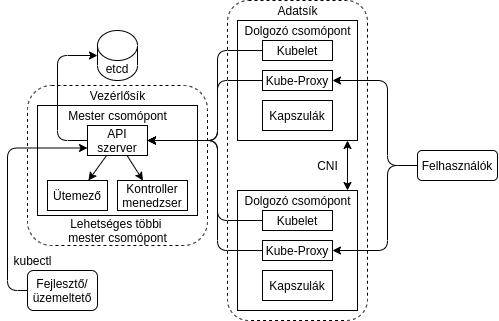
\includegraphics[width=1\textwidth, keepaspectratio]{figures/k8s_architecture.png}
	\caption{Kubernetes klaszter felépítése}
	\label{fig:achitecture}
\end{figure}

Egy Kubernetes klaszter kettő részből áll egy vezérlő- és egy adatsíkból, ahol a 
vezérlősíkban szereplő mester csomópontok tudják vezérleni az adatsíkban 
lévő dolgozó csomópontokat és a fejlesztők vagy üzemeltetők a mester által
hirdetett API-n (Application Programming Interface) keresztül képesek parancsokat
kiadni. Míg a dolgozó csomópontokon futó alkalmazáshoz a felhasználók csak az 
általuk hirdetett Kube-Proxy segítségével tudnak hozzáférni. 

A kapcsolat mester és dolgozó között az API szerver és a Kubelet kommunikációján
alapul. Ha a fejlesztő szeretne egy új alkalmazást telepíteni a klaszteren, akkor
szól az API szervernek, ami majd kiadja a megfelelő parancsokat a Kubelet-nek 
és majd az fogja a konténereket létrehozni.

\subsubsection{Vezérlősík}

A mester csomópont mindig a fő vezérlő egysége a klaszternek, mivel kezeli a 
munkafolyamatokat és irányítja a kommunikációt klaszteren belül. A 
\ref{fig:achitecture}-s ábrán látható vezérlősík tartalmazhat több mester csomópontot is 
a felsorolt komponensekkel, amivel lehet biztosítani a fejlesztők számára a folytonos 
elérést. A mester csomópont részei: 

\begin{itemize}
	\item \textbf{etcd}: Egy állandó kulcs-érték alapú adatbázis, ami tárolja 
	a klaszter konfigurációs beállításait és a klaszter állapotát. Fontos az a rész, 
	hogy ez egy állandó adatbázis, mivel ez a csomóponton fut és nem egy 
	kapszulában.   
	\item \textbf{API szerver}: Egy REST API (Representational State Transfer API) 
	szerver, ami hozzáférést biztosít a klaszterhez a klaszteren belül és azon kívül is. 
	Egyszerű HTTP üzenetekbe ágyazott JSON (JavaScript Object Notation) konfigurációkkal
	lehet beállítani, hogy mit csináljon a klaszterben. De a dolgozó csomópontok is ezen 
	keresztül küldenek frissítést az etcd-be. 
	\item \textbf{Ütemező}: Ez a komponens dönti el, hogy egy új kapszula melyik
	dolgozó csomóponton legyen létrehozva aszerint, hogy van-e megfelelő erőforrás
	az adott csomópontot megvalósító szerveren.
	\item \textbf{Kontroller menedzser}: Egy olyan állandóan futó folyamat, ami ellenőrzi,
	hogy a kapszulák bizonyos esetekben újrainduljanak vagy hogy egy ismétlődő 
	munkafolyamat időnénként lefusson helyesen. Ezt az API szerverrel kommunikálva
	képes megvalósítani. 
\end{itemize}

A \ref{fig:achitecture} ábrán látható, \texttt{kubectl} eszköz segítségével a fejlesztők 
és üzemeltetők képesek kommunikálni az API szerverrel. Ez az eszköz lényegében
megvalósítja a teljes HTTP kommunikációt az API szerverrel szóval sokkal könnyebben 
lehet vele lekérdezni információkat vagy új erőforrásokat létrehozni. 

\subsubsection{Adatsík}

Az adatsíkon futnak az úgynevezett dolgozók, amik igazából különálló szerverek,
amik rendelkeznek a \ref{fig:achitecture}-s ábrán szereplő komponensekkel és képesek 
futtatni valamilyen konténer kezelő alakalmázást, például Docker-t. Régebben a Docker
alapértelmezett konténer kezelője volt a Kubernetes-nek, de 2021-ben már nem követeli meg 
és bármilyen másik konténer kezelőt is be lehet állítani alapértelmezettnek. A fontosabb 
elemei az adatsíknak:

\begin{itemize}
	\item \textbf{Kubelet}: Felelős az egyes csomópontok futási állapotáért biztosítva, 
	hogy a csomóponton lévő összes konténer egészséges legyen. Gondoskodik az alkalmazás
	konténereinek indításáról, leállításáról és karbantartásáról, amelyek kapszulákba 
	vannak rendezve a vezérlősík utasítása szerint
	\item \textbf{Kube-Proxy}: Egy proxy és terheléselosztó megvalósítása, ami biztosítja
	a szolgáltatás elérhetőségét más hálózatok számára. Feladata, hogy a beérkező
	forgalmat a megfelelő konténerekhez irányítsa, amit különböző paraméterek szerint 
	képes megvalósítani.
	\item \textbf{Kapszulák}: A legkisebb menedzselhető egységek, amiket lehet telepíteni
	Kubernetes alatt. Egy kapszula több konténernek a csoportja, amik osztoznak a tárolási
	és hálózati erőforrásokon és specifikálja, hogy a konténerek hogyan fussanak. 
	\item \textbf{CNI (Container Network Interface)}: A kapszulák hálózati interfészeinek
	a beállítására lehet használni. Segítségével specifikálni lehet, hogy a kapszulák között milyen hálózatot használva legyen továbbítva a forgalom. 
\end{itemize}

\subsection{Erőforrások}

A \ref{fig:achitecture} architektúra csak a fő erőforrásokat mutatja be, amiken kívül
még rengeteg olyan erőforrással is rendelkezik, amik lehetővé teszik a konténerek 
menedzselésének egy új szintjét. 

Ismertetem, hogy a projekt szempontjából mely erőforrások lesznek még lényegesebbek. 
Viszont rengeteg olyan erőforrásról lehet többet olvasni \cite{kubeAPI}, amiket a 
Kubernetes segítségével lehet létrehozni.   

\begin{itemize}
	\item \textbf{Replikációs vezérlő}: Biztosítja, hogy egy meghatározott számú 
	kapszula replika fusson egyszerre, amivel biztosítja az alkalmazás magas szintű
	elérhetőségét. Ezáltal, ha túl sok kapszula fut, amikre nincs szükség, 
	akkor a felesleges kapszulák törlésre kerülnek, míg abban az esetben, ha az elvártnál
	kevesebb kapszula érhető el akkor újakat hoz létre. Mindazonáltal, ha egy kapszula 
	maga vagy az egyik konténere hibát eredményez, akkor újraindítja a benne lévő 
	konténer vagy a teljes kapszulát. 
	\item \textbf{Telepítő (Deployment}): Leír egy elvárt állapotot, ami alapján a
	replikációs vezérlő tudja, hogy milyen specifikáció szerint kell az új kapszulákat
	létrehozni vagy a létrehozandó kapszulák számát. 
	\item \textbf{DaemonSet}: Biztosítja, hogy az összes vagy néhány csomópont 
	futtassa egy meghatározott kapszula másolatát. Ezáltal, ha egy új dolgozó csomópont 
	csatlakozik a klaszterhez, akkor ez a kapszula automatikusan megjelenik rajta. 
	Tipikusan valamilyen tárolási vagy monitorozási feladatot ellátó kapszulát szokás 
	ilyen módon létrehozni, de a későbbiekben látni fogjuk, hogy az L7mp ugyan ezzel a 
	módszerrel hozza létre a bejárati pontokat a csomópontokon.
	\item \textbf{DNS (Domain Name System)}: Tárolja a klaszterben szereplő minden 
	kapszula és szolgáltatás IP címét illetve a hozzájuk kapcsolódó tartomány nevüket 
	is.  
	\item \textbf{Szolgáltatás}: Egy absztrakt módja az alkalmazást futtató kapszulák
	kiexponálásának a hálózaton keresztül. Mivel a kapszulák halandóak így nem mindig
	ugyanazon a címen lesznek elérhetőek a rajtuk futtatott alkalmazások. A megoldás
	erre, ha egy címke alapján hozzárendeljük őket egy szolgáltatáshoz, ami mindig 
	elérhető lesz ugyanazon a címen és képes elosztani a forgalmat több kapszula között.
	A forgalomirányítást a szolgáltatások a Kubernetes DNS szolgáltatása miatt tudják 
	megvalósítani. Mivel minden kapszula rendelkezik egy tartománynévvel és ez a 
	Kubernetes DNS leírójában szerepel egy hozzá tartozó IP címmel.
	\item \textbf{Bejárat (Ingress gateway)}: Egy olyan API objektum, ami kezeli a 
	külső hozzáférést különböző szolgáltatásokhoz a klaszteren belül. Ezáltal a bejövő 
	forgalmat könnyen lehet szűrni illetve típusától, tartalmától függően más és más 
	szolgáltatásokhoz lehet irányítani. 
	\item \textbf{Egyéni erőforrás definíció (Custorm Resource Definition)}: A 
	Kubernetes API egy olyan kiterjesztése melynek során új fajta erőforrás definíciókat
	lehet definiálni, amik bővítik a Kurbenetes funkcionalitását.
	\item \textbf{Pótkocsi (Sidecar)}: Mivel egy kapszula több konténert is tartalmazhat
	és ezek a konténerek megosztják a hálózatukat így létre lehet hozni egy olyan 
	konténert, ami csak a hálózati forgalom kezelésével foglalkozik. Segítségévével lehet 
	szűrni, hogy milyen forgalom juthat csak el az alkalmazást futtató konténerhez. Mivel 
	elsőnek  mindig ezen pótkocsin fog áthaladni a forgalom majd lokális hálózaton átadja 
	az alkalmazásnak. Ezek a pótkocsik általában valamilyen proxyk szoktak lenni. 
	\item \textbf{RBAC (Role-based access controll)}: Ha több fejlesztő vagy üzemeltető
	fér hozzá az API szerverhez, akkor egyénenként meglehet mondani, hogy kinek milyen 
	művelet végrehajtására van joga. Például korlátozható, hogy ki képes új
	erőforrásokat létrehozni. Viszont a felhasználók mögött sokszor nem egy élő 
	személy van, hanem egy alkalmazáshoz van hozzárendelve. Ezáltal az alkalmazás 
	esetlegesen képes a klaszteren belülről erőforrásokat kezelni.
	\item \textbf{Operátor}: Olyan bővítések, amikkel egyéni erőforrások menedzselése
	valósítható meg. De emellett különböző eseményeknél lehet bizonyos folyamatokat 
	elindítani. Példának okáért, ha egy kapszula létrejön, akkor beállíthatjuk, hogy
	rendelkezzen mindig egy adott címkével.
	\item \textbf{Szolgáltatásháló (Service Mesh)}: Meghatározza, hogy a klaszter 
	különböző részei hogyan kommunikáljanak egymással. Ezt általában a pótkocsikkal és 
	egy operátorral valósítják meg. A pótkocsik fognak rendelkezni azokkal a 
	beállításokkal, hogy a mellettük futó konténer milyen forgalmat fogadhat és az 
	operátor fog arról gondoskodni, hogy a résztvevő kapszulák pótkocsijai mindig a 
	megfelelő beállításokkal jöjjenek létre.
\end{itemize}

\section{L7mp}

Az L7mp egy kísérleti alkalmazásréteg és több protokollt támogató szolgáltatás- proxy és 
háló keretrendszer. A hangsúly a több protokoll támogatásán van, amely lehetővé teszi, 
hogy sok szállítási- és alkalmazásréteg béli protokollt natívan támogasson és ne csak a 
szokásos TCP/HTTP protokollokat. Lehetővé teszik emellett még a protokollok közötti 
konvertálást is, amivel könnyen lehet alkalmazási rétegű protokollokat konvertálni 
szállításiba és vissza is.

Az L7mp egy vezérlő- és adatsíkból áll: az adatsíkot az L7mp proxy valósítja meg, míg a 
vezérlőt egy operátor, ami kezeli az L7mp proxy példányokat.

Ha egy másik szoftverhez kellene hasonlítani az L7mp-t, akkor leginkább az Istio-hoz 
lehetne, hiszen felépítésében nagyon hasonló elemeket használ, mint az Istio. Szóval 
akinek van valamilyen tapasztalata az Istio-val az könnyen kiismeri magát az L7mp-vel is.

Szeretném megemlíteni, hogy Dr. Rétvári Gábor vezetésével a nyári gyakorlati időm alatt 
és jelenlegi munkámként ennek a szoftvernek a tesztelésével  illetve fejlesztésével 
foglalkozom. 

\subsection{L7mp, mint proxy}

Az L7mp proxy egy olyan programozható proxy, ami nagyon hasonlóan működik, mint az Envoy, 
ami egy széleskörűen használt leginkább alkalmazási réteget támogató proxy. A különbség 
az L7mp proxy és az Envoy között, hogy az L7mp proxy a szállítási réteg protokolljait  
támogatja jobban míg az Envoy inkább az alkalmazásréteg protokolljait képes jobban  
kezelni.Emellett az L7mp proxy képes protokollok közötti átalakítást végezni, ami sok 
esetben hasznos lehet. Ez a funkcionalitás az architektúra leírása után fog jobban 
megmutatkozni.

A L7mp proxy egy magas szintű keretrendszerben íródott, ezért nagyon egyszerűen 
lehet új funkciókkal bővíteni. Ez a keretrendszer a Node.js, ami egy JavaScript
futtató környezet a Google Chrome V8-s JavaScript motorjára építve. Ez szerencsés 
választás a már említett egyszerű bővíthetőség miatt, de amiatt is, hogy
könnyen lehet vele aszinkron módon programozni. Mivel nincsenek blokkoló műveletek,
amiket külön szálon kellene futtatni. De behozza azt a hátrányt is, hogy a 
JavaScript miatt lassabb az L7mp, mint az Envoy, ami C++-ban van írva. 

A lassúság kiküszöbölésére jelenleg vannak munkálatok, amik elsősorban azt 
célozzák meg hogy a csomagok feldolgozása nem a felhasználói névtérben kerüljenek
végrehajtásra, hanem kernel szinten. 

Az L7mp proxy használható szimplán Node.js-sel indítva, mivel elérhető az NPM (Node 
Package Manager) tárolóban. Az indítása a \ref{lst:nodeL7mp} paranccsal történik: 

\begin{lstlisting}[caption=L7mp indítása Node.js segítségével, label=lst:nodeL7mp]
node l7mp-proxy.js -c config/l7mp-minimal.yaml -l warn -s
\end{lstlisting}

A \ref{lst:nodeL7mp} parancs kiadása után a minimális L7mp konfigurációval és a 
figyelmeztetés naplózási szinten fog elindulni az L7mp proxy. A minimális konfiguráció 
létre fog hozni egy REST API szervert, amin keresztül a későbbiekben újabb L7mp 
beállításokat lehet megadni.

Ezen felül a Docker-t is támogatja, ami alapértelmezetten a \ref{lst:nodeL7mp} parancsot 
fogja egy konténerben futtatni.

\subsubsection{Felépítés}

Mivel az L7mp proxy tervezése során az Envoy volt a minta, így főbb elemei között 
szerepelnek ugyanolyan vagy hasonló elemek. A legfontosabb építőkockái az L7mp proxynak 
felsorolásra és kifejtésre kerülnek alább: 

\begin{itemize}
	\item \textbf{Munkamenet (Session)}: Munkameneteket nem lehet manuálisan létrehozni,
	mivel ezek akkor generálódnak, amikor egy figyelő forgalmat kap és azt 
	továbbítja valamerre. Egy munkamenet információkat tartalmaz a csomagok típusáról,
	forrás címéről és céljáról. Emellett a munkamenet objektum felelős azért is, hogy a
	a benne lévő objektumok tudják, hogy a hozzájuk beérkező csomagokat fel kell 
	dolgozniuk. 
	\item \textbf{Figyelő (Listener)}: Definiálni lehet vele egy cím és port párost, hogy
	adott protokollal rendelkező csomagokra figyeljen és dolgozza fel őket. A feldolgozás
	alatt azt a folyamatot kell érteni, hogy meghatározza mely L7mp klaszterhez kerüljön 
	a csomag, szűri a bejövő csomagokat valamilyen paraméter alapján, ha lehet. Ez 
	általában a csomagok fejlécében szereplő információk, vagy a munkamenetben 
	megtalálható bármilyen érték alapján történhet. 
	\item \textbf{L7mp klaszter (Cluster)}: A végpontok egy gyűjteménye, ami képes 
	forgalmat elosztani közöttük. Az elosztás történhet nagyon egyszerűen, amikor mindig 
	egy lista élén álló végpont kapja a forgalmat, de történhet HashRing módszerrel is. 
	Amikor egy kulcs szerint történik a végpont kiválasztása. Ez egy hasznos funkció, 
	mivel fix kulcs mellett, minden csomag ugyanahhoz végponthoz fog kerülni. 
	\item \textbf{Végpont (Endpoint)}: A csomag végállomása, ami lehet a már csomagokat
	feldolgozó alkalmazás vagy egy másik figyelő is.
	\item \textbf{Szabály (Rule)}: Szabályokat a figyelőkben lehet létrehozni, amikkel
	be lehet állítani, hogy mi legyen a célja a beérkező csomagoknak vagy meg lehet vele 
	azt is határozni, hogy a fejléc mely paraméterét mire módosítsa. 
	\item \textbf{Útvonal (Route)}: Meghatározza a célt, ami általában egy L7mp klaszter. 
	Az útvonalak mindig a szabályokon belül vannak, hiszen a szabályok határozzák meg a 
	célt. De ezen felül még be lehet azt is állítani, hogy a bejövő csomagok milyen 
	útvonalon jussanak el az L7mp klaszterig és milyenen vissza. Ezáltal a bejövő és 
	kimenő forgalmat teljesen más útvonalon lehet irányítani.
\end{itemize}

A Munkamenet kivételével ezeket az elemeket egy jól definiált API leírás alapján 
könnyedén lehet konfigurálni. Tehát az L7mp proxy egyszerű HTTP \texttt{POST} üzenetekkel 
beállítható.

\subsubsection{Programozása}

Az L7mp programozása történhet konfigurációs fájlból és REST API hívásokon keresztül
egyaránt. Viszont az L7mp indításához szükség van egy alapkonfigurációra, mivel
anélkül nem fog létrejönni a kontroller figyelő, ami biztosítja az API 
láthatóságát. A \ref{lst:minL7mp} kódrészleten látható, hogyan lehet egy ilyen induló 
konfigurációt létrehozni YAML (YAML Ain't Markup Language) fájllal.

\begin{lstlisting}[caption=L7mp minimális konfiguráció, label=lst:minL7mp]
admin:
  log_level: info
  log_file: stdout
  access_log_path: /tmp/admin_access.log
listeners:
  - name: controller-listener
    spec: { protocol: HTTP, port: 1234 }
    rules:
      - action:
          route:
            destination:
              name: l7mp-controller
              spec: { protocol: L7mpController }
\end{lstlisting}

A konfigurációt részről részre kifejtem. Az első része, az \texttt{admin}, ahol
a naplózás szintjét és helyét lehet meghatározni. A következő szintek vannak:
\texttt{silly}, \texttt{verbose}, \texttt{info}, \texttt{notice}, \texttt{warn}, 
\texttt{error}, \texttt{silent}, amik ebben a sorrendben egyre kevesebb információt 
naplóznak. A \texttt{silly} kiírja a beérkező csomagok  tartalmát is, míg az 
\texttt{info} már csak munkafolyamat leírásáig működik.

Az utána következő részben létre jön a \texttt{controller-listener}, ami helyi hálózaton 
az \texttt{1234} porton hirdeti a REST API pontot, amin keresztül később új 
konfigurációkat lehet megadni. Ehhez egy olyan L7mp klaszter van használva, amelyhez nem 
tartozik semmilyen definiált végpont. Ebben az L7mp klaszterben egy automatikusan 
létrejövő API szerepel, amihez beérkeznek a figyelőn keresztül a HTTP kérések. 

Ez az API megvalósítja a teljes CRUD-t (Create, Read, Update, Delete) minden
komponensre, amivel tudunk létrehozni, olvasni, frissíteni és törölni komponenseket. 
Minden komponenshez tartozik egy útvonal, ami így tevődik össze, ha a \ref{lst:minL7mp} 
példát nézzük: \texttt{http://127.0.0.1:1234/api/v1/listeners}. Ha erre a címre egy 
\texttt{POST} üzenetben YAML vagy JSON konfigurációt küldünk, akkor az létre fog jönni a 
L7mp proxyn belül. Még egy hasznos funkció ebben a megvalósításban az a rekurzív lekérés, 
aminek során egy \texttt{GET} üzenettel és az URI paraméterekben a 
\texttt{recursive=true} beállításával az összes figyelő definíciója a bennük lévő többi 
objektummal együtt részletesen megkapható. Kétféle  API leírás létezik az L7mp-hez egy az 
önálló L7mp proxyhoz \cite{proxy} és egy olyan, amit a Kubernetes operátor tud használni 
\cite{kubeProxy}. Azért létezik kétféle API leírás, mert az elsőnek létrehozott nem volt 
teljesen kompatibilis a Kubernetes-sel így keletkezett még egy. Jövőbeni tervek között 
szerepel ezek egységesítése.

\begin{lstlisting}[caption=L7mp konfigurálása API-n keresztül, label=lst:confL7mpAPI]
curl -iX POST --header 'Content-Type:text/x-yaml' --data-binary @- <<EOF  http://localhost:1234/api/v1/listeners
listener:
  spec:
    protocol: WebSocket
    port: 2000
  rules:
    - action:
        route:
          destination:
            spec:
              protocol: UDP
                port: 3000
            endpoints:
              - spec:
                  address: 127.0.0.1
EOF
\end{lstlisting}

A \ref{lst:confL7mpAPI} hívásban látható, hogy létrehozunk egy figyelőt, ami a 
\texttt{127.0.0.1:2000}-s címen fog WebSocket csomagokat várni, majd azokat UDP-re 
konvertálva továbbküldeni a \texttt{127.0.0.1:3000}-s címre.

Ezen a példán látszik igazán, hogy milyen egyszerű az L7mp-vel a protokoll konverzió,
mert ilyen rövid beállítással kettő nagyon különböző protokoll között lehet 
átalakítást végezni.

\subsection{L7mp, mint szolgáltatásháló}

A szolgáltatásháló egy olyan keretrendszert foglal magában, amivel a különböző 
mikroszolgáltatások közötti kommunikációt lehet meghatározni. Ezek a szolgáltatások 
konténerek, amik rendelkeznek egy olyan API interfésszel, amin keresztül lehet 
őket programozni. Emellett olyan szolgáltatásokat lehet igénybe venni a Kubernetes 
klaszteren belül, mint a szolgáltatás felderítés, terhelés elosztás és felügyelhetőség. 
Ezeken kívül még rengeteg más funkcióval szokott rendelkezni egy szolgáltatásháló, de 
ezeket lehet mondani a legnépszerűbbeknek.

A megvalósításához minden mikroszolgáltatásnak azaz kapszulának rendelkeznie kell 
egy pótkocsival, ami egy adott L7mp proxyt fog futtatni. Ez a konténer lesz minden esetben
a belépési pont az alkalmazáshoz. Ezeket az L7mp proxykat valahogyan dinamikusan kell 
tudni konfigurálni, amit egy operátor segítéségével lehet megtenni. A használt L7mp 
proxyknak rendelkezni kell egy olyan interfésszel, amin keresztül lehet őket 
konfigurálni. Az L7mp szolgáltatásháló esetében egyértelműen az L7mp proxyk lesznek használva, aminél az \ref{lst:confL7mpAPI} részben láttuk hogyan lehet egy API 
interfészt definiálni, amin keresztül \texttt{POST} hívásokkal lehet új beállításokat 
eszközölni.

De ezeket a beállításokat valamilyen módon közölni kell az L7mp operátorral, amihez 
szükség van egyéni erőforrásokra. Az L7mp esetében ezek az erőforrások sorra a 
VirtualService, Target és Rule. Ezekben lehet olyan beállításokat megadni, amiket
később az L7mp operátora képes leképezni az L7mp proxyk számára érthető konfigurációra.

\subsubsection{Virtuális szolgáltatás - VirtualService}

Egy virtuális szolgáltatás az absztrakt megvalósítása egy szerveroldali foglalatnak 
(socket). A benne definiált figyelő a meghatározott kapszulák pótkocsijaiban létre fog 
jönni és kezelni tudja hozzá beérkező forgalmat. 

Egy ilyen erőforrás két fő részből áll, az egyik a kapszulák kiválasztásáért felel míg
a másik azért, hogy milyen definíció kerüljön alkalmazásra a kijelölt kapszulákban.
A kiválasztás mindig valamilyen címke alapján történik, amivel rendelkezik a kapszula. 
Ezt viszont többször lehet használni egy definíción belül, mert meg lehet vele határozni,
hogy a figyelő mely kapszulákon jöjjön létre és azt is, hogy a végpontok mely kapszulák 
legyenek. 

A másik fontos része maga a figyelő definíciója, ami nagyon hasonló, mint az L7mp proxy
esetében, de itt már vannak Kubernetes specifikus elemek is, mint a szelektor,
amivel a kapszulák kiválasztása történik meg. De ilyen az is, hogy egy Kubernetes 
erőforrásra név szerint lehet hivatkozni, amit majd az L7mp operátor feloldva fog az L7mp
proxy konténereknek átadni.

\subsubsection{Target - Cél}

Egy cél definiálásával a kliens oldali foglalatokat lehet meghatározni. Ezeken 
a címeken várja az alkalmazás vagy egy másik figyelő a forgalmat. Mivel egy cél 
lényegében egy L7mp klasztert valósít meg, így ez is a végpontokat tárolja, azzal a 
különbséggel, hogy célnál a végpontok a kapszulák, szolgáltatások vagy virtuális 
szolgáltatások is lehetnek. 

A felépítése hasonlóan néz, ki mint a virtuális szolgáltatásoknak, tehát van egy 
szelektor, hogy mely pótkocsikon legyen elérhető az adott L7mp klaszter. Illetve az L7mp 
klaszter definíciója. 

Ebben a definícióban lehet megadni, hogy a milyen protokollú csomagokat fogad, végpontokat
és a terheléselosztás beállításait. A végpontok kiválasztása szintén egy szelektorral
történik, ami a Kubernetes erőforrások címkéi alapján választ. A másik fontos beállítása
a terheléselosztás, ami alapértelmezett esetben, mindig a nyilván tartott kapszulák 
közül az elsőnek fogja irányítani a csomagokat. Viszont be lehet állítani úgy is, hogy
egy a csomag fejlécében lévő mező alapján irányítsa a csomagokat. Ez a megoldás a
HashRing megoldást, használja, amivel elérhető, hogy egy kulcs alapján mindig 
ugyan az a végpont kapja meg a csomagokat. 

\subsubsection{Rule - Szabály}

Szabályokkal lehet összekötni figyelőket az L7mp klaszterekkel. De ebben az esetben lehet 
különálló CRD-ben szabályokat létrehozni és azokat többször felhasználni. Ennélfogva 
átláthatóbbá és kontrollálhatóbbá válik a szolgáltatásháló használata. 

Használatukkal lehet szűrni a csomagokat forráscímük, fejlécük és még nagyon sok más 
paraméter szerint. \texttt{JSON predicate} objektumokkal lehet szűrni az csomagokat, 
amivel könnyen lehet komplex szűrési feltételeket meghatározni különböző paraméterek 
alapján. Ha egy csomag megfelel minden kitételnek, akkor a definiált művelet szerint fog 
tovább haladni a csomag.

\subsubsection{Példa a szolgáltatásháló használatára}

A \ref{lst:crdL7mp} kódrészletben ugyan az van megvalósítva, mint a \ref{lst:confL7mpAPI}
API hívással, azzal a különbséggel, hogy most a szolgáltatásháló lett konfigurálva. 

\begin{lstlisting}[caption=L7mp szolgáltatásháló konfigurálása CRD-n keresztül, label=lst:crdL7mp]
cat <<EOF | kubectl apply -f -
apiVersion: l7mp.io/v1
kind: VirtualService
metadata:
  name: ws-listener
spec:
  selector:
    matchLabels:
      app: l7mp-ingress
  listener:
    spec:
      WebSocket:
        port: 2000
    rules:
      - action:
          route:
            destinationRef: /l7mp.io/v1/Target/default/udp-target
---
apiVersion: l7mp.io/v1
kind: Target
metadata:
  name: udp-target
spec:
  selector:
    matchLabels:
      app: l7mp-ingress
  cluster:
    spec:
      UDP:
        port: 3000
    endpoints:
      - { spec: address: 127.0.0.1 }
EOF
\end{lstlisting}

Részleteiben megnézve a \ref{lst:crdL7mp} kódot látszik, hogy a figyelő beállításai a 
virtuális szolgáltatásban vannak definiálva, míg az L7mp klaszter a cél objektumban van
megvalósítva. A szelektor mindkét CRD-ben az \texttt{l7mp-ingress} kapszula, ami 
rendelkezik egy L7mp proxyval, így mindkét erőforrás leképezésre kerül az L7mp operátor 
által az \texttt{l7mp-ingress} kapszulában található L7mp proxyba. Innentől kezdve minden 
WebSocket csomag, ami a kapszula 2000-s portjára érkezik az továbbítva lesz annak a 
lokális 3000-s portjára UDP csomagként. 

A célnál a végpontok megadásakor is lehet szelektort használni, amivel egyszerre több
kapszula is megadható végpontként. 

\section{rtpengine}

Az rtpengine egy Sipwise  által fejlesztett a Kamailio-hoz szánt RTP proxy, ami nem csak 
forgalmat képes irányítani, hanem a beérkező csomagokat transzformálni is. Emellett olyan 
funkciókkal is rendelkezik, amikkel tudjuk a hívások minőségét monitorozni, rendelkezésre 
állóságát és biztonságát növelni. A következő funkciókat érdemes jobban kifejteni a 
\cite{rtpengine} közül: 

\begin{itemize}
	\item Tud IPv4 és IPv6 címeket kezelni és közöttük média forgalmat továbbítani. 
	\item Állítható port tartomány. 
	\item Több interfész használata. 
	\item Kernel szintű csomagtovábbítás a kisebb késleltetés és processzor használat 
	miatt.
	\item HTTP, HTTPS és WebSocket interfész támogatottság.
	\item Médiafolyamok felvétele. 
	\item Híváshoz szükséges statisztikák számítása.
	\item Transzkódolás és újracsomagolás.
	\item SDP csomagok teljes újraírása. 
\end{itemize}

\subsection{Kernel és felhasználói tér}

Az rtpengine alapvetően a felhasználói térben működik így ilyenkor mindent ott csinál, ami
magasabb késeltetést és processzor használatot igényel. Az oka ennek, hogy mikor egy 
csomag érkezik a hálózati interfészre az áthalad a kernelen a fájlleíróig. Ha odajutott 
egy csomag, akkor a hozzá kapcsolódó folyamatot értesíti, ami ebben az esetben az 
rtpengine, hogy van mit leolvasni onnét. Ennek során a csomag átkerül a kernelből a 
felhasználói térbe, ami egy nagyon drága művelet. Ha feldolgozásra került a csomag, 
akkor ugyanezen az útvonalon fog kimenni. Ez azért nagy probléma, mert az RTP protokoll 
UDP-t használ, így rengeteg kis csomag érkezik folyamatosan, ami nagy terhelést jelent 
a szerver számára. 

Ezzel szemben, ha használjuk a megfelelő modult, akkor a beérkező csomagok nem kerülnek 
át a felhasználói térbe így kevesebb erőforrás kerül felhasználásra. Ezt úgy éri el az 
rtpengine, hogy egy hívás kiépítése során \texttt{iptables} szabályokat hoz létre, 
amikben definiálja, hogy adott portra érkező forgalom hova legyen továbbítva. 

Az \texttt{iptables} egy olyan eszköz, amivel a linux kernelben lehet létrehozni 
táblákat szabályokkal, amik IP szinten képesek szűrni a forgalmat. 

\subsection{Transzkódolás}

Transzkódolás alatt azt a folyamatot értjük, amikor egy adott formátumú videó- vagy 
hanganyag egy másik formátumba való átalakítása történik. Ezt jelenleg az rtpengine 
csak hanggal tudja megvalósítani. 

Alapvetően elérhető ez a funkció, de ki is kapcsolható teljesen. Ugyanakkor az, hogy 
elérhető az rtpengine nem avatkozik bele a hívott felek közötti kódolás megegyezésbe, 
így ha nincs közös kódolása a két félnek, akkor a hívás sikertelen lesz.

A transzkódlást az ng vezérlőprotokoll \texttt{transcoding} vagy \texttt{ptime} 
beállításával lehet az rtpengine tudtára adni. Tehát, ha a két félnek nincs közös 
kódolása, de az rtpengine mind a kettő számára képes egy olyat nyújtani, amit elfogad, 
akkor a hívás sikeresen kiépül.

Ha aktív transzkódolás van, akkor az SDP-ből kikerül minden olyan kódolási eljárás, amit 
nem támogatnak a kliensek. Emellett ezt nem lehet kernel szinten továbbítani, ezért 
mindenképpen a felhasználói térben lesznek ezek a csomagok feldolgozva.

Ezek a formátumok vannak támogatva: \texttt{G.711} (a-Law és µ-Law), \texttt{G.722}, 
\texttt{G.723.1}, \texttt{G.729}, \texttt{Speex}, \texttt{GSM}, \texttt{iLBC}, 
\texttt{Opus}, \texttt{AMR} (keskeny és széles sávú)

\subsection{ng vezérlőprotokoll}

Ahhoz, hogy bizonyos funkciók engedélyezve legyenek az rtpengine-ben kifejlesztettek 
egy vezérlési protokollt, amibe a SIP proxy beágyazva áttudja adni az SDP törzset 
az rtpengine-nek, ami az SDP üzeneteknek egy módosított verzióját küldi vissza a 
klienseknek.

Ez a vezérlőprotokoll bencode formátumban küldi el az üzeneteket. Ez nagyon hasonló
felépítéssel rendelkezik, mint a JSON, viszont sokkal egyszerűbb és gyorsabb a kódolása 
és dekódolása. Hátránya a JSON-nal szemben, hogy kevésbé olvasható.

Fontos megjegyezni, hogy ilyen üzeneteket a rtpengine a következő protokollokon képes fogadni: UDP, TCP, HTTP, HTTPS, WebSocket, WebSocket Secure. De a projekt során a 
HTTP, HTTPS és WebSocket protokollokat nem lehet használni a használt rtpengine és 
Kamailio verzió miatt, amiről a \ref{sec:rtpengine} fejezetben lesz részletesen szó.

Minden ilyen üzenet két részből áll. Egy sütiből, ami ebben az esetben azonosítóként
funkciónál és egy bencode szótárból, ami legalább egy parancsot tartalmaz az 
alábbiak közül. A felsorolás nem teljes \cite{rtpengineng}, csak a téma szempontjából 
fontosokat emeltem ki.

\begin{itemize}
	\item \textbf{ping}: Ellenőrizhető, hogy az rtpengine elérhető-e. Egyetlen helyes 
	válasz van rá, az pedig a \textbf{pong}.
	\item \textbf{offer}: A hívó fél adatait rögzíti.
	\item \textbf{answer}: A hívott fél adatait rögzíti. 
	\item \textbf{delete}: Egy adott azonosítóval rendelkező hívást lehet törölni.
	\item \textbf{query}: Egy hívás részleteit lehet lekérdezni. 
	\item \textbf{statistics}: Egy adott azonosítóval rendelkező hívásról lehet 
	statisztikát lekérdezni. 
\end{itemize} 

\subsection{Beállítás}

\begin{lstlisting}[caption=rtpengine konfigurációja, label=lst:confRtpe]
[rtpengine]
interface=192.168.1.106
foreground=true
log-stderr=true
listen-ng=192.168.1.106:22222
port-min=23000
port-max=32768
log-level=7
\end{lstlisting}

Ezzel a következő dolgokat állítom be: 

\begin{itemize}
	\item \textbf{interface}: Megadja az RTP helyi hálózati interfészét. Legalább
	egyet meg kell adni, de több is megadható. Ez ez interfész fogja kezelni a 
	médiaforgalmat. 
	\item \textbf{listen-ng}: A vezérlő üzeneteket ezen a címen várja. 
	\item \textbf{port-min és port-max}: Az UDP média forgalom számára lefoglalható
	portok tartománya. 
	\item \textbf{Többi}: Naplózás szempontjából érdekesek csak. 
\end{itemize}

\section{Kamailio}

A Kamailio egy nyílt forráskódú SIP Signaling Server. A Kamailio-t alapvetően nagy 
rendszerek skálázhatóságára tervezték, de használható cégek és egyének számára is.

A használatához általában szükség van valamilyen Kamailio által támogatott adatbázisra,
de elméletileg lehet adatbázis nélkül is használni, de akkor elvesztünk bizonyos 
funkciókat. Ezért az ajánlott adatbázist használtam hozzá, ami egy lokálisan futó 
\texttt{MySQL} szerver. Ebbe az adatbázisba olyan táblákat tárol, mint regisztrált 
felhasználók és aktív hívások, de ezen felül még sok mást is. 

Ezenkívül az általam használt beállításokat a \texttt{kamailio.cfg} fájlban lehet megadni,
ami három részből áll. A használt dokumentációból \cite{kamailio} jól látszik, hogy a fájl szerkesztése nagyon sok szempontból emlékeztet egy programozási nyelvre 
\texttt{C} szerű elemekkel.  

Az első a \textbf{globális paraméterek}, ahol leginkább környezeti változókat lehet 
definiálni, amikkel lehet kontrollálni, hogy a konfiguráció mely része fusson le illetve
értékeket is lehet hozzájuk rendelni. 

Aztán jönnek a \textbf{modul beállítások}, ahol az alapértelmezett modulokhoz tudunk plusz
modulokat betölteni és beállítani. Ezen modulok segítségével lehet oly módon konfigurálni 
a Kamailio szervert, hogy képes legyen használni rtpengine-t vagy RTP proxyt. Tehát, ha 
se rtpengine se RTP proxy nincs engedélyezve és telepítve, akkor a Kamailio a két SIP 
klienst közvetlen fogja összekötni.

Végül van az \textbf{irányítási blokk}, ahol különböző SIP üzenetekre lehet megmondani, 
hogy mi történjen velük, ha beérkeznek a hálózati interfészre. Itt be tudjuk állítani 
azt, hogy az \texttt{INVITE} üzenetek esetén az ng vezérlőprotokollon keresztül állítsa 
be a hívást az rtpengine szerveren.

\section{Hívásfelépítés Kubernetes nélkül}

Ahhoz, hogy a valóshoz hasonló infrastruktúrát lehessen létrehozni, több 
számítógépet kellett valahogyan összekapcsolni és rajtuk a megfelelő szoftvereket
elindítani. A környezet megvalósításához egy VirtualBox nevezetű virtuális gépeket
létrehozó és kezelő alkalmazást választottam. Indoka a választásomnak azon
alapult, hogy egyszerű használni és ingyenes.

De csak a virtuális gépek jelenléte még nem jelenti azt, hogy ezek tudnak egymással 
kommunikálni. Ezért a telepítés során Brideged adapter használtam minden virtuális gép 
esetében, ami kiszolgáló számítógép hálózati kártyáján keresztül képes elérni az 
internetet. Ezzel hálózattal tökéletesen lehetett abban az esetben, ha az rtpengine nem 
Kubernetes környezetben működött. Később át kellett térnem kiszolgáló adapteres hálózat 
használatára különben a lokális Kubernetes klasztert nem látták a SIP kliensek. 

A kliensek tekintetében is az ingyenességre és az egyszerű használatra törekedtem, 
de fontos volt még az a szempont is, hogy lehessen parancssorosan hívást kezdeményezni
és fogadni. Ezekkel az a funkciókkal rendelkezett a Linphone nevezetű kliens, ami
rendkívül sok beállítást engedélyez ingyenesen a felhasználóinak. Számomra a következő
funkciók voltak nagyon hasznosnak: \texttt{wav} fájl lejátszása hívás közben, használt 
kódolás kiválasztása és a hívás rögzítése. A \texttt{wav} fájl lejátszása, azért egy 
fontos funkció, mert így nem kell törődni azzal, hogy a mikrofon keresztül valamilyen 
hangot tudjon rögzíteni.

Egy általános VoIP híváshoz szükség van legalább egy SIP szerverre, ami képes a 
felhasználókhoz kapcsolatos információkat kezelni. Erre a célra Kamailio-t használok, 
mivel ehhez készítették az rtpeninge-t. Ezáltal kézenfekvő volt a használata, de 
elméletileg lehet más SIP szervereket is használni az rtpengine-l. A másik fontos, de 
egyértelmű tényező az maga az rtpengine.

\subsection{Kommunikáció}

Az normál architektúrához a már említett VirtualBox-szal létrehoztam négy virtuális gépet,
amik \texttt{Ubuntu 20.04} operációs rendszer használnak. Ezek közül egyre telepítésre 
került a Kamailio, egyre az rtpengine és kettőre egy-egy Linphone kliens. A klienseknek 
azért van szüksége két különböző virtuális gépre, mert Linphone-ból nem lehet kettőt
párhuzamosan futtatni egy gépen.

A Kamailio beállítása során az alapkonfigurációt használtam, mivel a Kamailio 5.4-s verziója már alapértelmezetten tartalmazza az rtpengine-hez szükséges beállításokat. Nekem csak a megfelelő globális paramétereket kell beállítani illetve az rtpengine modul beállításainál a rtpengine elérhetőségét megadni. A használt rtpengine beállításai a használt IP címek kivételével teljes mértékben azonosak az \ref{lst:confRtpe} konfigurációt leíró fájllal. 

A Kamailio-hoz még felhasználókat kellett regisztrálni, amikkel a kliensek képesek 
csatlakozni hozzá. Az ehhez használt parancs az \ref{lst:addUserKamailio} látható, ahol 
az első paraméter a felhasználó neve majd utána a jelszava.

\begin{lstlisting}[caption=Felhasználó hozzáadása Kamailio-hoz, label=lst:addUserKamailio]
kamctl add A 123
\end{lstlisting}

Abban az esetben, ha a Kamailio-t futtató szerver IP címe \texttt{192.168.99.102}, akkor az így létrejött felhasználó azonosítója a következő lesz: \texttt{sip:A@192.168.99.102}. Ezzel a címmel lehet a Linphone kliensekben regisztrálni ezt a felhasználót. 

De hogyan is kell beállítani a Linphone klienseket? Erre add választ a \ref{lst:setupLinphone} részletben megadott parancsok. 

\begin{lstlisting}[caption=Linphone beállítása, label=lst:setupLinphone]
register sip:A@192.168.99.102 192.168.99.102 123
soundcard use files
play /home/user/input.wan
\end{lstlisting}

Az első sorral kerül regisztrálásra a felhasználó, ahol az első argumentum adja meg a 
felhasználó azonosítóját, második a tartomány címét és a végül a jelszó kerül átadásra. 
Ezután, ha újraindításra kerül a Linphone, akkor automatikusan megpróbálja a definiált
felhasználót regisztrálni. 

A következő sor azt adja meg, hogy ne használjon semmilyen hangkártyát és csak a 
harmadik sorban specifikált fájlt játssza le a hívásban részvevő feleknek.

\begin{figure}[!ht]
	\centering
	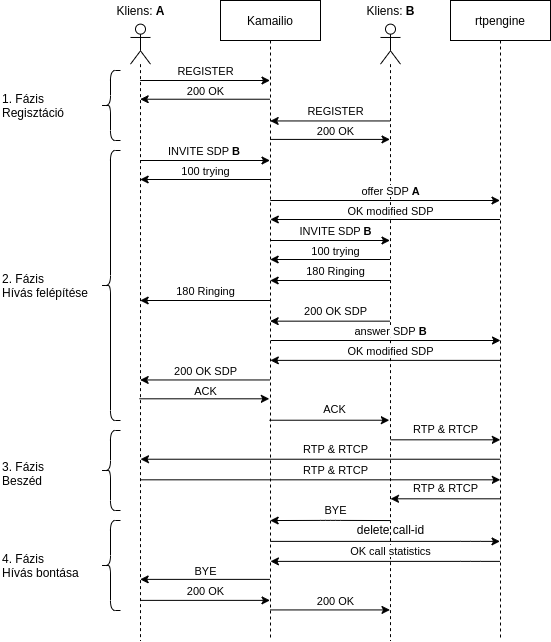
\includegraphics[width=0.9\textwidth, keepaspectratio]{figures/basic_call_flow.png}
	\caption{Kubernetes nélküli hívásfelépítés}
	\label{fig:callflow}
\end{figure}

Az \ref{fig:callflow} ábra segítségével ismertetem a hívásfelépítés részeit.  Az ábrán 
látható egy teljes hívás folyamata a regisztrációtól egészen a hívás bontásáig. Négy 
részre bontottam a hívást annak érdekében, hogy könnyebb legyen a megértése.

Az első rész a regisztráció, amelynek során a felhasználók csatlakoznak a SIP szerverhez.
Ilyenkor a kliens \texttt{SIP REGISTER} üzenetet küld a szervernek, amikkel hozzáadni, 
törölni és lekérdezni lehet a felhasználó adait szerverről. Ha létezik a felhasználónak 
fiókja a szerveren, viszont még nem jelentkeztek be az adott eszközről akkor az első 
alkalommal egy \texttt{401 Unauthorized} üzenettel tér vissza, ami felszólítja a klienst, 
hogy adja meg a hitelesítéshez szükséges felhasználói azonosítót és jelszót, amit egy 
újabb \texttt{SIP REGISTER} üzenetben fog újraküldeni titkosítva. Ha minden megfelelt, 
akkor \texttt{200 OK} üzenetet kap vissza a kliens, ami jelzi, hogy minden rendben és tud 
hívásokat kezdeményezni. Az ábrán szereplő folyamat nem tartalmazza a \texttt{401} 
státusz üzenetet, mert már többször használva volt a kliens azon a virtuális gépen.

A következő rész pedig már a konkrét hívás kezdeményezése és felépítése. A hívást az 
\textbf{A} felhasználó kezdeményezi \textbf{B} irányába egy \texttt{INVITE} üzenettel, 
ami tartalmaz egy SDP üzenetet is. Ez az SDP egy olyan protokoll, amivel a híváshoz 
kapcsolódó információkat lehet továbbítani, mint például a támogatott média formátumok 
listája illetve a hívott fél elérhetőségei. Mivel ebben az esetben \textbf{B} felhasználó 
címe létezik a szerveren így a szerver \texttt{100 trying} üzenettel jelzi 
\textbf{A}-nak, hogy elkezdte a hívást felépíteni. Erre azért van szükség, hogy a kliens 
ne próbálkozzon újra a hívás felépítésével.

A szerver ilyenkor küld egy \texttt{offer} üzenetet az rtpengine felé, aminek legalább 
tartalmaznia kell az \textbf{A} által küldött SDP üzenetet, hívásazonosítót és a SIP 
üzenet \texttt{From} mezőjét, ami az \textbf{A} azonosítója. Erre az rtpengine egy 
módosított SDP üzenetet küld vissza a szervernek, amiben módosítja a cél címet és portot 
a sajátjára. Ezáltal minden RTP üzenet elsőnek az rtpengine-hez fog elmenni és majd onnét 
megy tovább \textbf{B}-nek.

Ha ez is sikeresen megtörtént, a szerver átveszi a hívás kezdeményező szerepét a 
\textbf{B}-vel szemben. Szóval küld egy \texttt{INVITE} üzenetet neki, amiben szerepel 
\textbf{A} azonosítója, de a csatlakozást leíró mező az rtpengine címe lesz. A 
\texttt{trying} üzenet ebben az esetben is ugyan azt jelenti, mint mikor az \textbf{A} 
kezdeményezett. De itt már szerepel a \texttt{180 ringing}, amivel lehet jelzi, hogy 
feldolgozásra került az \texttt{INVITE}. Majd ugyan ez az üzenetet megkapja \textbf{A} 
is. 

Ha \textbf{B} elfogadta a hívást, akkor \texttt{200 OK} státusszal jelez a szervernek, 
amiből a SIP szerver tudja, hogy \texttt{answer}-t kell küldenie az rtpengine felé, 
amivel a hívás teljesen ki fog épülni az rtpengine-ben is. Az \texttt{answer} igazából 
ugyanazt a funkciót valósítja meg, mint az \texttt{offer}. Mivel az rtpengine kapott 
\texttt{offer}-t és \texttt{answer}-t is, így a hívást kiépítheti és az előzőleg 
lefoglalt négy porton képes fogadni a forgalmat, amit feldolgozva tovább küld. Azért 
foglal le négy port, mert felenként kell egy páros számú port az RTP forgalomnak és egy 
páratlan számú az RTCP-nek. Végül pedig egy \texttt{SIP ACK} üzenettel van értesítve mind 
a két fél arról, hogy a hívás sikeresen kiépült és elkezdhetnek beszélni. 

Mivel már létezik a hívás, lehet küldeni a forgalmat az rtpengine adott 
portjaira. Ahol a legegyszerűbb esetben annyi történik, hogy az \textbf{A}-hoz rendelt
RTP porton kapott csomagokat kiküldi a \textbf{B}-hez a hozzárendelt portról. Ugyanez
történik RTCP esetében is. 

Mikor vége a hívásnak, akkor megkezdődik a hívás lebontása egy \texttt{BYE SIP} 
üzenettel. Aminek hatására a SIP szerver egy \texttt{delete} üzenetet ad ki az rtpengine 
felé, ami tartalmazza a hívás azonosítóját. Ekkor törlődik minden a híváshoz kapcsolódó 
információ és a számukra kinyitott portok is lezárnak. De a rtpengine válaszában 
szerepelnek a hívásról információk, amik alapján könnyen lehet statisztikákat készíteni 
például a hívások átlagos hosszáról vagy minőségéről.
%%----------------------------------------------------------------------------   
\chapter{Használt eszközök bemutatása}
%---------------------------------------------------------------------------- 

\section{Kubernetes}

A Kubernetes egy nyílt forráskódú konténer kezelő platform, amivel automatizálni
lehet a legtöbb feladatot, ami a fejlesztés, karbantartás vagy skálázással 
kapcsolatos. A Google fejlesztette eredetileg, de jelenleg a Cloud Native
Computing Foundation - CNCF vette át a karbantartását. 

Kubernetes fürtöt létrehozhatunk lokálisan a saját szerveren is vagy felhőben,
ami lehet publikus, privát vagy hibrid hozzáférésű. Viszont azt figyelembe 
kell venni, hogy egy Kubernetes fürtöt nem egyszerű kiépíteni lokálisan, 
szóval ha nem szükséges, akkor lehet használni felhőszolgáltatók Kubernetes 
motorjai, mint az Amazon AKS, Linode LKE vagy a Google GKE szolgáltatása.
Ilyenkor egy teljes fürtöt, ami az általunk beállított paramétereket használja.

\subsection{Felépítése}

Egy Kubernetes fürt kettő részből áll egy vezérlő- és egy adatsíkból, ahol a 
vezérlősíkban szereplő mester csomópontok tudják vezérleni az adatsíkban 
lévő dolgozó csomópontokat és a fejlesztők vagy üzemeltetők a mester által
hirdetett API-n keresztül képesek parancsokat kiadni. Míg a dolgozó 
csomópontokon futó alkalmazáshoz a felhasználók csak az általuk hirdetett 
Kube-Proxy segítségével tudnak hozzáférni. 

A kapcsolat mester és dolgozó között az API szerver és a Kubelet kommunikációján
alapul. Ha a fejlesztő szeretne egy új alkalmazást telepíteni a fürtön, akkor
szól az API szervernek, ami majd kiadja a megfelelő parancsokat a Kubelet-nek 
és majd az fogja a konténereket létrehozni. Amiről az API szervert értesítve 
tudja meg a fejlesztő, hogy amit csinált az létrejött. \\

A következőkben az alábbi ábra alapján részletesen kifejtem a Kubernetes 
részeit. 

\begin{figure}[!ht]
	\centering
	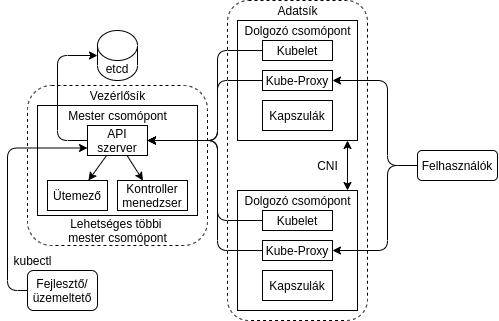
\includegraphics[width=1\textwidth, keepaspectratio]{figures/k8s_architecture.png}
	\caption{Kubernetes fürt felépítése}
	\label{fig:HVSpaces}
\end{figure}

\subsubsection{Vezérlősík}


\subsubsection{Adatsík}

\subsection{Fontos Kubernetes elemek}

Ahhoz, hogy jobban meglehessen érteni, mi hogyan működik a Kubernetes világban,
ezért az alábbi fogalmakat fontos ismerni:

\begin{itemize}
	\item \textbf{Vezérlősík (Controle Plane)}: Folyamatok gyűjteménye melyek 
	kontrollálják a Kubernetes csomópontokat.
	\item \textbf{Csomópont (Node)}: A vezérlősík által kiadott feladatokat 
	végrehajtó szerverek.
	\item \textbf{Kapszula (Pod)}: Több konténer gyűjteménye, melyek egyetlen
	csomóponton futnak és egy IP címem és más dolgokon osztoznak.
	\item \textbf{Replikációs vezérlő (Replication Controller)}: Kontrollálja,
	hogy egy kapszulából hány azonos fusson a fürtön.  Ezek a másolatok majdnem 
	mindenben azonosak egymással.
	\item \textbf{Szolgáltatás (Service)}: A hozzárendelt kapszulák, vagyis 
	végpontok között képes a forgalmat elosztani. Emellett címkék alapján 
	képes automatikusan új végpontokat regisztrálni vagy törölni.
	\item \textbf{Telepítő (Deployment)}: Deklaratívan frissíti a kapszulákat 
	és a replikációs vezérlőt. Így, ha valamilyen indok miatt egy kapszulában
	lévő konténer hibát generál, akkor újraindítja vagy esetlegesen törli a 
	kapszulát és egy teljesen újat indít. 
	\item \textbf{Egyéni erőforrás definíció (Custom Resource Definition)}:
	A Kubernetes API (Application Programming Interface) kiterjesztésére 
	lehet használni.
	\item \textbf{Operátor (Operator)}: Egy alkalmazás specifikus kontroller, 
	ami kibővíti a Kubernetes API funkcionalitását. 
	\item \textbf{Kubelet}: Csomópontokon futó szolgáltatás, ami a konténer 
	leírások alapján biztosítja, hogy a definiált konténerek fussanak.
	\item \textbf{kubectl}: Parancssoros eszköz, amivel a Kubernetes-t lehet 
	konfigurálni.
\end{itemize}

\section{L7mp}

Az L7mp egy több protokollt támogató szolgálatatás haló es porxy, amellyel 
könnyen lehet a legtöbb szállítás és alkalmazás réteg béli protokollt továbbítani
illetve fordítani. Esetünkben a szolgáltatás háló funkcionalitása lesz a 
fontosabb, de ettől függetlenül kitérek a proxy részére is, mert minden a 
legtöbb Kubernetes erőforrás használni fogja a proxy részét is. 

A szakdolgozat szempontjából még érdemes megemlíteni, hogy ez egy még nagyon 
erősen fejlesztés alatt álló projekt, szóval a vele megvalósított megoldások 
nem biztos, hogy tudják garantálni a megbízhatóságot. \\

Beszerzése ennek a szoftvernek rendkívül egyszerű. Ha csak a proxy-ra van 
szükség, akkor ugyan úgy telepíthető, mint bármelyik NPM (Node Package Manager)
csomag vagy használható Docker konténerként is, aminek a képfájlja elérhető 
ezzel a címkével: \textbf{l7mp/l7mp}. 

De a szolgáltatás háló használatához már muszáj Helm-t használni, amivel 
teljes Kubernetes architektúrákat lehet könnyedén megvalósítani. Ennek a 
menete megtalálható az L7mp oldalán is. 

\subsection{L7mp, mint proxy}

Működésében, nagyon hasonló az Envoy-hoz, ami egy a lyft által készített és 
nagyon sok helyen használt proxy. Azzal a különbséggel, hogy az L7mp inkább 
az alsóbb rétegbeli protokollokat támogatja, ezért a szállítási réteg legtöbb 
protokollja támogatva van és lehet bizonyos értékeik alapján irányítani a 
proxy-n áthaladó forgalmat. Példának okáért lehet olyat csinálni, hogy egy
Unix Domain Socket (UDS) foglalaton figyeli a forgalmat, majd azt WebSocket-re
átfordítva küldi tovább. 

Ezzel szemben nagyon sok olyan tulajdonsággal nem rendelkezik, ami megtalálható
az Envoy-ban. Ilyennek tudható be, hogy az alkalmazás réteg protokolljai nincsenek 
teljesen támogatva vagy nem rendelkeznek olyan szintű implementációval. Ami 
még egy nagyobb hátránya, hogy nem tud olyan gyors lenni az L7mp, mint az Envoy.
Ennek a legnagyobb oka, hogy az L7mp Node.js keretrendszerben íródott, ami a 
JavaScript miatt sokkal lassabb, mint a C++ nyelven íródott Envoy.

\subsubsection{Felépítése}

Mint már említve volt az L7mp rendkívül hasonlít az Envoy-ra és ez nincs másképp 
a felépítésben is. Szóval ennek a proxy-nak a használatához a következő 
építőköveket kell jobban ismerni: \textbf{Session}, \textbf{Listeners}, \textbf{Clusters}, \textbf{Endpoints}, \textbf{Rules}, \textbf{Routes}.\\

A Session (munkamenet) mindig akkor jön létre, amikor valamelyik Listener 
bejövő forgalmat kap. Erre azért van szükség, hogy a láncban meghatározott 
elemeknek mindig a megfelelő függvénye hívódjon meg és a hibák megfelelően 
legyenek kezelve. 

A Listener vagy magyarul figyelő úgy működik, mint egy szerver, ami bizonyos 
szempontok alapján figyelik a hozzájuk beérkező forgalmat és azt továbbítják
egy adott címre. Ezek a címek a Cluster-ek (fürtök) szoktak lenni, amiknek a 
működése közel azonos a Listener-ével, mivel ezek is a rajtuk beérkező forgalmat
adják tovább, azzal a kivétellel, hogy ezek nem láthatóak a proxy-n kívülről.

Végük a forgalom utolsó állomása az Endpoint vagyis végpont, ami már egy konkrét
cím, ahol figyel az általunk beállított alkalmazás. Fontos megjegyezni, hogy 
ezek az útvonalak kétirányúak, szóval a proxy képes kimenő forgalmat is ugyanúgy 
kezelni, mint a bejövőt. 

Amik a fentebb említett elemeket összeköti az a Rule (szabály) és a Route (irány),
A szabály által lehet különböző paraméterekre szűrni vagy hozzáadni. Ez azért egy 
nagyon hasznos funkció, mert ezáltal egy Session-n belül képes UDP forgalmat 
címkékkel ellátni és ezen címkék alapján megfelelő irányba továbbítani a 
forgalmat.

\subsubsection{Programozása}

Az L7mp indításához mindig biztosítani kell neki egy alapkonfigurációt, ami 
lehet általában egy L7mpController Listener-t és egy Cluster-t jelent, amin 
keresztül információkat tudunk szerezni az éppen futó proxy-ról vagy új 
elemeket lehet egyszerűen létrehozni. 

Új elemek hozzáadásához csak a proxy címére kell egy POST HTTP (HyperText Transfer 
Protocol) hívást indítani, aminek keretében a konfigurációt YAML (YAML Ain't Markup 
Language) vagy JSON (JavaScript Object Notation) formátumban tudjuk átadni.
Erre alább lehet látni egy nagyon egyszerű példát, ahol az L7mp a következő címen 
figyel: http://localhost:1234. 

\begin{lstlisting}
	curl -iX POST --header 'Content-Type:text/x-yaml' --data-binary @- <<EOF  http://localhost:1234/api/v1/listeners
	listener:
	  spec:
	    protocol: WebSocket
	    port: 2000
	  rules:
	    - action:
	        route:
	          destination:
	            spec:
  	              protocol: UDP
	              port: 3000
	            endpoints:
	              - spec:
	                  address: 127.0.0.1
	EOF
\end{lstlisting}

A fenti hívásban az látható, hogyan lehet egy Listener-t minden attribútumával 
létrehozni a proxy-n belül. Ez most a 127.0.0.1:2000-s címen figyel és minden 
bejövő forgalmat UDP-n továbbít a 127.0.0.1:3000-s címre. De ettől sokkal több
mindent is belehet állítani könnyedén. 

\subsection{L7mp, mint szolgáltatás háló}

Szolgáltatás háló alatt igazából egy olyan operátora kell gondolni, ami a Kubernetes
API-n (Application Programming Interface) keresztül képes L7mp proxy-k halmazát 
kezelni. Ezáltal könnyen tudjuk az L7mp-t, mint ingress gateway használni és 
mint sidecar az alkalmazás kapszulákban.

Ez az operátor három CRD-t használnak a L7mp proxy-k programozására, amik a következők:
\textbf{VirtualService}, \textbf{Target}, \textbf{Rule}. Ezek sorban a következő proxy 
elemeknek felelnek meg: \textbf{Listener}, \textbf{Cluster}, \textbf{Rule}. \\ 

Egy \textbf{VirtualService} az absztrakt megvalósítási egy szerver oldali foglalatnak címnek. 
Ezenfelül egy VirtualService mögött mindig áll egy Kubernetes szolgáltatás, ami 
szolgáltatja a végpontok címét vagy címkéit az elérhetőség miatt.

VirtualService részei: 

\begin{itemize}
	\item Egy szelektor, ami kiválasztja a definiált kapszulákat címkék alapján.
	\item Egy Listener, ami kezeli a beérkező forgalmat. 
	\item (Opcionális) Egy szabálylista, ami tartalmazhat újraírást, érték ellenőrzést
	és meghatározza a célt. 
	\item (Opcionális) További beállítások.  
\end{itemize}

A kliens oldali foglalatot mindig a \textbf{Target} valósítja meg, de beállíthatóak még a 
következő tulajdonságok is: terhelés elosztás, lokális cím lefoglalása, illetve 
meghatározhatnak még végpontot is, amihez a kliensnek csatlakoznia kellene. Ez 
lehet egy másik Target, konkrét cím vagy egy Listener is. Ezenfelül még meglehet 
határozni a bejövő és kimenő forgalom útját is. Így különböző útvonalakat lehet 
könnyen megvalósítani. 

Ha egy Target egyedi névvel rendelkezik, akkor más L7mp erőforrás könnyen 
felhasználhatja a névére való hivatkozással. Ez mind a három CRD-re igaz, de ha
nem határozunk meg egy konkrét nevet, akkor a rendszer automatikusan generál 
egyet minden erőforrásnak. 

%--------------
% PLACE OF RULE
%--------------
%%---------------------------------------------------------------------------- 
\chapter{Hívásfelépítés Kubernetes nélkül}
%---------------------------------------------------------------------------- 

Ahhoz, hogy a valóshoz hasonló infrastruktúrát lehessen létrehozni, több 
számítógépet kellett valahogyan összekapcsolni és rajtuk a megfelelő szoftvereket
elindítani. A környezet megvalósításához egy VirtualBox nevezetű virtuális gépeket
létrehozó és kezelő alkalmazást választottam. Indoka a választásomnak azon
alapult, hogy egyszerű használni és ingyenes.

De csak a virtuális gépek jelenléte még nem jelenti azt, hogy ezek tudnak egymással
kommunikálni. Ezért a telepítés során csak sima Brideged adapter használtam minden
virtuális gép esetében, ami kiszolgáló számítógép hálózati kártyáján keresztül
képes elérni az internetet. Ezzel hálózattal tökéletesen lehetett tesztelni
akkor, ha az rtpengine nem Kubernetes környezetben működött. Később át kellett
térnem kiszolgáló adapteres hálózat használatára különben a lokális Kubernetes 
fürtöt nem látták a SIP kliensek. 

A kliensek tekintetében is az ingyenességre és az egyszerű használatra törekedtem, 
de fontos volt még az a szempont is, hogy lehessen parancssorosan hívást kezdeményezni
és fogadni. Ezekkel az a funkciókkal rendelkezett a Linphone nevezetű kliens, ami
rendkívül sok beállítást engedélyez ingyenesen a felhasználóinak. Számomra a következő
funkciók voltak nagyon hasznosnak: wav fájl lejátszása hívás közben, használt kódolás
kiválasztása és a hívás rögzítése. A wav fájl lejátszása, azért egy fontos funkció, mert
így nem kell törődni azzal, hogy a mikrofon keresztül valamilyen hangot tudjon rögzíteni.

Egy általános VoIP híváshoz szükség van legalább egy SIP szerverre, ami képes a felhasználókhoz
kapcsolatos információkat kezelni. Erre a célra Kamailio-t használok, mivel ehhez készítették
az rtpeninge-t. Így kézenfekvő volt a használata, de elméletileg lehet más SIP szervereket
is használni az rtpengine-l. A másik fontos, de egyértelmű tényező az maga az rtpengine, 
amiről a következő fejezetben lesz részletesen szó. 

\section{rtpengine}

Az rtpengine egy Sipwise  által fejlesztett a Kamailio-hoz szánt RTP 
proxy, ami nem csak forgalmat képes irányítani, hanem a beérkező csomagokat transzformálni is.
Emellett olyan funkciókkal is rendelkezik, amikkel tudjuk a hívások minőségét monitorozni, 
rendelkezésre állóságát és biztonságát növelni. A következő funkciókat érdemes 
jobban kifejteni: 

\begin{itemize}
	\item Tud IPv4 és IPv6 címeket kezelni és közöttük média forgalmat továbbítani. 
	\item Állítható port tartomány. 
	\item Több interfész használata. 
	\item Kernel szintű csomagtovábbítás a kisebb késleltetés és processzor használat miatt.
	\item HTTP, HTTPS és WebSocket interfész támogatottság.
	\item Médiafolyamok felvétele. 
	\item Híváshoz szükséges statisztikák számítása.
	\item Transzkódolás és újracsomagolás.
	\item SDP csomagok teljesen újraírása. 
\end{itemize}

\subsection{Kernel és felhasználói tér}

Az rtpengine alapvetően a felhasználói térben működik így ilyenkor mindent ott csinál, ami
magasabb késeltetést és processzor használatot igényel. Az oka ennek, hogy mikor egy csomag
érkezik a hálózati interfészre az áthalad a kernelen a fájlleíróig. Ha odajutott egy 
csomag, akkor a hozzá kapcsolódó folyamatot értesíti, ami ebben az esetben az rtpengine, hogy
van mit leolvasni onnét. Ennek során a csomag átkerül a kernelből a felhasználói térbe és 
ami egy nagyon drága művelet. Ha feldolgozásra került a csomag, akkor ugyanezen az útvonalon
fog kimenni. Ez azért nagy probléma, mert az RTP protokoll UDP-t használ és így rengeteg 
kis csomag érkezik folyamatosan, ami nagy terhelést jelent a szerver számára. 

Ezzel szemben, ha használjuk a megfelelő modult, akkor a beérkező csomagok nem kerülnek át a 
felhasználói térbe így kevesebb erőforrás kerül felhasználásra. Ezt úgy éri el az rtpengine,
hogy egy hívás kiépítése során \textbf{iptables} szabályokat hoz létre, amikben definiálja, hogy
adott portra érkező forgalom hova legyen továbbítva. 

Az \textbf{iptables} egy olyan eszköz, amivel a linux kernelben lehet létrehozni 
táblákat szabályokkal, amik IP szinten képesek szűrni a forgalmat. 

%A választás azért erre a proxy-ra esett, mert folyamatos támogatottsága van, sok helyen 
%használják illetve sok olyan funkcióval rendelkezik, ami a projekt szempontjából fontos.

%Ilyen és legszükségesebb funkciója a Redis támogatottsága, amivel egyes hívásokhoz 
%lehet minden szükséges adatot elmenteni és ezen adatok alapján más rtpengine példányok 
%tudják frissíteni a hívásaikat. Így, ha egy az egyik szerver megáll és nem tudja tovább
%kezelni a hívásokat, akkor egy terhelés elosztó áttudja irányítani az összes hívást 
%más szerverekhez, amik ezáltal rendelkeznek a híváshoz szükséges információkkal. 
%
%A Redis támogatottság már létezett, viszont csak akkor, ha az rtpengine konfigurálásánál
%pontosan ismerjük az összes többi rtpengine címét. Alapesetben ezek az információk 
%rendelkezésre állnak, viszont Kubernetes környezetben ezek mind változékonyak. Sosem 
%tudjuk pontosan megjósolni, hogy egy kapszula, ami egy rtpengine szervert futtat milyen
%címmel fog létrejönni. 
%
%Ezt a problémát orvosolta részben Oded Arbell, aki egy Pull Request keretein belül 
%benyújtott egy nulla tudású Redis skálázhatóság funkciót. Mint a neve is utal rá 
%ezzel a megoldással úgy lehet az infrastruktúrába új rtpengine szervereket felvenni, 
%hogy nem kell ismerni a többi résztvevő szerver címét. De ez még mindig csak részben 
%oldotta meg a problémát ugyanis ha van két rtpengine szerverünk, akkor az egyikhez 
%beérkező hívásnál csak azon a szerveren fognak kinyílni a megfelelő portok, amire a 
%hívás beérkezett. Így, ha ez a szerver leáll, akkor a másik nem tudja kezelni a forgalmat,
%mert nincs nyitva egyik szükséges portja sem. 
%
%Megoldásképpen egy kicsit bele kellett nyúlnom ebbe a kódba és beállítani, hogy frissítésnél
%nyisson ki minden olyan portot, ami a hívás információi között szerepel. Így elértem 
%egy olyan fajta redundanciát, amivel a fentebb leírt váltás jól működik. \\
%
%Amit még érdemes megemlíteni, hogy az rtpengine képes kettő különböző módban működni.
%Tud simán a felhasználói névtérben futni, amikor a transzkódolást és az adatok 
%továbbítását is ott végzi el és tudja a kernel névteret is használni, amikor a 
%továbbítást a kernel névtérben végzi. Így processzor erőforrást lehet spórolni, mert
%nem kell a szervernek azt a drága műveletet minden csomagnál elvégeznie, hogy 
%a kernel névtérből felhasználóiba teszi át a csomagokat. 

\subsection{Transzkódolás}

Transzkódolás alatt azt a folyamatot értjük, amikor egy adott formátumú videó- vagy 
hanganyag egy másik formátumba való átalakítása történik. Ezt jelenleg az rtpengine 
csak hanggal tudja megvalósítani. 

Alapvetően elérhető ez a funkció, de ki is kapcsolható teljesen. Ugyanakkor az, hogy 
elérhető az rtpengine nem avatkozik bele a hívott felek közötti kódolás megegyezésbe, 
így ha nincs közös kódolása a két félnek, akkor a hívás sikertelen lesz.

A transzkódlást az ng vezérlőprotokoll \textit{transcoding} vagy \textit{ptime} beállításával
lehet az rtpengine tudtára adni. Így, ha a két félnek nincs közös kodekje, de az rtpengine
mind a kettő számára képes egy olyat nyújtani, amit elfogad, akkor a hívás sikeresen kiépül.

Ha aktív transzkódolás van, akkor az SDP-ből kikerül minden olyan kódolási eljárás, amit nem támogatnak
a kliensek. Emellett ezt nem lehet kernel szinten továbbítani, ezért mindenképpen a 
felhasználói térben lesznek ezek a csomagok feldolgozva.

Ezek a formátumok vannak támogatva: G.711 (a-Law és µ-Law), G.722, G.723.1, G.729, Speex, 
GSM, iLBC, Opus, AMR (keskeny és széles sávú)

\subsection{ng vezérlőprotokoll}

Ahhoz, hogy bizonyos funkciók engedélyezve legyenek az rtpengine-ben kifejlesztettek 
egy vezérlési protokollt, amibe a SIP proxy beágyazva áttudja adni az SDP törzset 
az rtpengine-nek, ami ennek a SDP üzenetnek a módosított verzióját fogja visszaküldeni
a klienseknek.

Ez a vezérlőprotokoll bencode formátumban küldi ki el az üzeneteket. Ez nagyon hasonló
felépítéssel rendelkezik, mint a JSON, viszont sokkal egyszerűbb és gyorsabb a kódolása 
és dekódolása. Ami hátránya a JSON-l szemben, hogy kevésbé olvasható.

Fontos megjegyezni, hogy ilyen üzenetek képes fogadni az rtpengine ezeken a protokollokon: 
UDP, TCP, HTTP, HTTPS, WebSocket, WebSocket Secure. De a projekt során a HTTP, HTTPS és 
WebSocket protokollokat nem lehet használni a használt rtpengine és kamailio 
verzió miatt, ami az architektúra fejezetben kiderül, hogy miért nem.

Minden ilyen üzenet két részből áll. Egy sütiből, ami ebben az esetben azonosítóként
funkciónál és egy bencode szótárból, ami legalább egy parancsot tartalmaz az 
alábbiak közül. A felsorolás nem teljes, csak a téma szempontjából fontosokat 
emeltem ki.

\begin{itemize}
	\item \textbf{ping}: Ellenőrizhető, hogy az rtpengine elérhető-e. Egyetlen helyes 
	válasz van rá, az pedig a \textbf{pong}.
	\item \textbf{offer}: A hívó fél adatait rögzíti.
	\item \textbf{answer}: A hívott fél adatait rögzíti. 
	\item \textbf{delete}: Egy adott azonosítóval rendelkező hívást lehet törölni.
	\item \textbf{query}: Egy hívás részleteit lehet lekérdezni. 
	\item \textbf{statistics}: Egy adott azonosítóval rendelkező hívásról lehet statisztikát
	lekérdezni. 
\end{itemize} 

\subsection{Beállítás}

\begin{lstlisting}[caption=rtpengine konfigurációja, label=lst:confRtpe]
	[rtpengine]
	interface=192.168.1.106
	foreground=true
	log-stderr=true
	listen-ng=192.168.1.106:22222
	port-min=23000
	port-max=32768
	log-level=7
\end{lstlisting}

Ezzel a következő dolgokat állítom be: 

\begin{itemize}
	\item \textbf{interface}: Megadja az RTP helyi hálózati interfészét. Legalább
	egyet meg kell adni, de több is megadható. Ez ez interfész fogja kezelni a 
	médiaforgalmat. 
	\item \textbf{listen-ng}: A vezérlő üzeneteket ezen a címen várja. 
	\item \textbf{port-min és port-max}: Az UDP média forgalom számára lefoglalható
	portok tartománya. 
	\item \textbf{Többi}: Naplózás szempontjából érdekesek csak. 
\end{itemize}

\section{Kamailio}

A Kamailio egy SIP Signaling Server nyílt forráskódú megvalósítása. Amit nagy rendszerek
skálázhatóságára terveztek, de használható cégek és egyének számára is.

A használatához általában szükség van valamilyen Kamailio által támogatott adatbázishoz,
de elméletileg lehet adatbázis nélkül is használni, de akkor elvesztünk bizonyos funkciókat. 
Ezért az ajánlott adatbázist használtam hozzá, ami egy lokálisan futó mysql szerver. Ebbe 
az adatbázisba olyan táblákat tárol, mint regisztrált felhasználók és aktív hívások, de 
ezen felül még sok mást is. 

Ezenkívül az általam használt beállításokat a \textit{kamailio.cfg} fájlban lehet megadni,
ami három részből áll. 

Az első a \textbf{globális paraméterek}, ahol leginkább környezeti változókat lehet 
definiálni, amikkel lehet kontrollálni, hogy a konfiguráció mely része fusson le illetve
értékeket is lehet hozzájuk rendelni. 

Aztán jönnek a \textbf{modul beállítások}, ahol az alapértelmezett modulokhoz tudunk plusz
modulokat betölteni és beállítani. Ez azért egy fontos rész, mert a Kamailio alapvetően 
nem rtpengine-re van beállítva, hanem annak az előző verziójához, ami az rtpproxy. Ami 
nem kerül telepítésre az kamailio-val együtt. Így, ha se rtpengine se rtpproxy nincs,
akkor az kamailio két SIP klienst közvetlen fogja összekötni.

Végül van az \textbf{irányítási blokk}, ahol különböző SIP üzenetekre lehet megmondani, hogy mi
történjen velük, ha beérkeznek a hálózati interfészre. Itt betudjuk állítani azt, hogy
az \textbf{INVITE} üzenetek esetén az ng vezérlőprotokollon keresztül állítsa be a hívást
az rtpengine szerveren.

\section{Kommunikáció}

Az normál architektúrához a már említett VirtualBox-l létrehoztam négy virtuális gépet,
amik Ubuntu 20.04 operációs rendszer használnak. Ezek közül egyre telepítésre került 
a Kamailio, egyre az rtpengine és kettőre egy-egy Linphone kliens. A klienseknek azért
van szüksége két különböző virtuális gépre, mert Linphone-ból nem lehet kettőt
párhuzamosan futtatni egy gépen.

A Kamailio beállítása során egy a publikus Github tárolóban található konfigurációt
használtam, mivel abban beállításra került az rtpengine használata. Így nekem 
csak a modul inicializáció során kellett megadnom az rtpengine címét és annak portját. 
Viszont az rtpengine beállítása teljes mértékben azonos a \ref{lst:confRtpe} megadott konfigurációval azzal a különbséggel, hogy más IP címek szerepelnek benne.

Amit még a Kamailio-val kellett tenni, hogy két felhasználókat kellett regisztrálni
különben nem lehetne a két kliens között hívást kezdeményezni. Az ehhez használt parancs
az \ref{lst:addUserKamailio} látható, ahol az első paraméter a felhasználó neve majd az azutáni a felhasználó jelszava.

\begin{lstlisting}[caption=Felhasználó hozzáadása Kamailio-hoz, label=lst:addUserKamailio]
kamctl add A 123
\end{lstlisting}

Abban az esetben, ha a Kamailio-t futtató szerver IP címe 192.168.99.102, akkor az 
így létrejött felhasználó azonosítója a következő lesz: sip:A@192.168.99.102. Ezzel a
címmel lehet a Linphone kliensekben regisztrálni ezt a felhasználót. 

De hogyan is kell beállítani a Linphone klienseket? Erre add választ a következő 
pár sor. 

\begin{lstlisting}[caption=Linphone beállítása, label=lst:setupLinphone]
register sip:A@192.168.99.102 192.168.99.102 123
soundcard use files
play /home/user/input.wan
\end{lstlisting}

Az első sorral kerül regisztrálásra a felhasználó, ahol az első argumentum adja meg a 
felhasználó azonosítóját, második a tartomány címét és a végül a jelszó kerül átadásra. 
Ezután, ha újraindításra kerül a Linphone, akkor automatikusan megpróbálja a definiált
felhasználót regisztrálni. 

A következő sor azt adja meg, hogy ne használjon semmilyen hangkártyát és csak a 
harmadik sorban specifikált fájlt játssza le a hívásban részvevő feleknek.  \\

\begin{figure}[!ht]
	\centering
	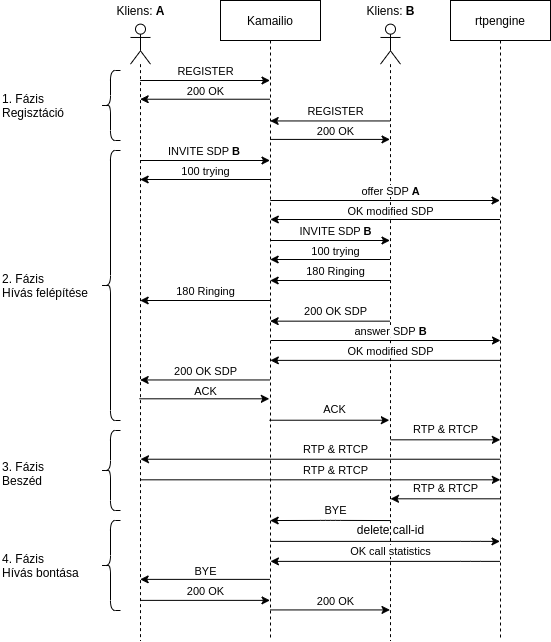
\includegraphics[width=0.9\textwidth, keepaspectratio]{figures/basic_call_flow.png}
	\caption{Kubernetes nélküli hívásfelépítés}
	\label{fig:callflow}
\end{figure}

Az \ref{fig:callflow} ábra segítségével a hívásfelépítés részeit.  Az ábrán látható 
egy teljes hívás folyamata a regisztrációtól egészen a hívás bontásáig. Négy részre 
bontottam a hívást annak érdekében, hogy könnyebb legyen a megértése.

Az első rész a regisztráció amelynek során a felhasználók csatlakoznak a SIP szerverhez.
Ilyenkor a kliens SIP REGISTER üzenetet küld a szervernek, amikkel hozzáadni, törölni és
lekérdezni lehet a felhasználó adait szerverről. Ha létezik a felhasználónak fiókja 
a szerveren, viszont még nem jelentkeztek be az adott eszközről akkor az első alkalommal 
egy 401 Unauthorized üzenettel tér vissza, ami felszólítja a klienst, hogy adja meg a 
hitelesítéshez szükséges felhasználói azonosítót és jelszót, amit egy újabb SIP REGISTER
üzenetben fog újraküldeni titkosítva. Ha minden megfelelt, akkor 200 OK üzenetet kap 
vissza a kliens, ami jelzi, hogy minden rendben és tud hívásokat kezdeményezni. Az ábrán
szereplő folyamat nem tartalmazza a 401-s üzenetet, mert már többször használva volt a 
kliens azon a virtuális gépen.

A következő rész pedig már a konkrét hívás kezdeményezése és felépítése. A hívást az 
\textbf{A} felhasználó kezdeményezi \textbf{B} irányába egy INVITE üzenettel, ami tartalmaz
egy SDP üzenetet is. Ez az SDP egy olyan protokoll, amivel a híváshoz kapcsolódó információkat
lehet továbbítani, mint például a támogatott média formátumok listája illetve a hívott fél
elérhetőségei. Mivel ebben az esetben \textbf{B} felhasználó címe létezik a szerveren így
a szerver 100 trying üzenettel jelzi \textbf{A}-nak, hogy elkezdte a hívást felépíteni. Erre
azért van szükség, hogy a kliens ne próbálkozzon újra a hívás felépítésével.

A szerver ilyenkor küld egy \textbf{offer} üzenetet az rtpengine felé, aminek legalább 
tartalmaznia kell az \textbf{A} által küldött SDP üzenetet, hívásazonosítót és a SIP üzenet
From mezőjét, ami az \textbf{A} azonosítója. Erre az rtpengine egy módosított SDP üzenetet küld
vissza a szervernek, amiben módosítja a cél címet és portot a sajátjára. Így minden RTP
üzenet elsőnek az rtpengine-hez fog elmenni és majd onnét megy tovább \textbf{B}-nek.

Ha ez is sikeresen megtörtént, a szerver átveszi a hívás kezdeményező szerepét a \textbf{B}-vel
szemben. Szóval küld egy INVITE üzenetet neki, amiben szerepel \textbf{A} azonosítója, de
a csatlakozást leíró mező az rtpengine címe lesz. A trying üzenet ebben az esetben is 
ugyan azt jelenti, mint mikor az \textbf{A} kezdeményezett. De itt már szerepel a 
\textbf{180 ringing}, amivel lehet jelzi, hogy feldolgozásra került az INVITE. Majd ugyan ez 
az üzenetet megkapja \textbf{A} is. 

Ha \textbf{B} elfogadta a hívást, akkor \textbf{200 OK}-l jelez a szervernek, amiből a
SIP szerver tudja, hogy \textbf{answer}-t kell küldenie az rtpengine felé, amivel a hívás teljesen
ki fog épülni az rtpengine-ben is. Az answer igazából ugyanazt a funkciót valósítja meg,
mint az offer. Mivel az rtpengine kapott offer-t és answer-t is, így a hívást kiépítheti
és az előzőleg lefoglalt négy porton képes fogadni a forgalmat, amit feldolgozva 
tovább küld. Azért foglal le négy port, mert felenként kell egy páros számú port az 
RTP forgalomnak és egy páratlan számú az RTCP-nek. Végül pedig egy SIP ACK üzenettel van
értesítve mind a két fél arról, hogy a hívás sikeresen kiépült és elkezdhetnek 
beszélni. 

Mivel már létezik a hívás így már lehet küldeni a forgalmat az rtpengine adott 
portjaira. Ahol a legegyszerűbb esetben annyi történik, hogy az \textbf{A}-hoz rendelt
RTP porton kapott csomagokat kiküldi a \textbf{B}-hez a hozzárendelt portról. Ugyanez
történik RTCP esetében is. 

Mikor vége a hívásnak, akkor megkezdődik a hívás lebontása egy BYE SIP üzenettel. Aminek
hatására a SIP szerver egy delete üzenetet ad ki az rtpengine felé, ami tartalmazza a hívás
azonosítóját. Ekkor törlődik minden a híváshoz kapcsolódó információ és a számukra kinyitott
portok is lezárnak. De a rtpengine válaszában szerepelnek a hívásról információk, amik alapján
könnyen lehet statisztikákat készíteni például a hívások átlagos hosszáról vagy minőségéről.

%----------------------------------------------------------------------------   
\chapter{Felhő alapú VoIP médiasík}
%---------------------------------------------------------------------------- 

\section{Kubernetes telepítése}

A Kubernetes architektúra tervezése során a fő szempont az volt, hogy teljes mértékben 
úgy nézzen ki kívülről, mintha egy szimpla rtpengine lenne. De mögötte egy 
mikroszolgáltatásokból álló alkalmazás legyen, mely képes az benne rejlő rtpengine-t 
megfelelően konfigurálni.

Ezt a Kubernetes klasztert a BME által szolgáltatott szervereken építettem ki, mi szám 
szerint 4 szervert tartalmaz melyek az \ref{fig:servers} elrendezésben vannak összekötve.

\begin{figure}[!ht]
	\centering
	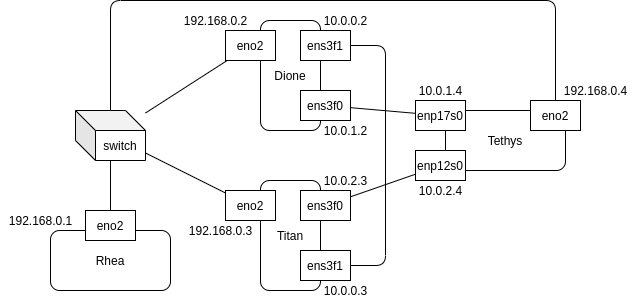
\includegraphics[width=1\textwidth, keepaspectratio]{figures/servers.png}
	\caption{Szerverek összeköttetése}
	\label{fig:servers}
\end{figure}

Az ábrán szereplő szervereket kettő részre lehet szétbontani, ahol az egyik
konkrétan a Kubernetes klaszter a másik pedig a forgalom generálására használatos.
Az előbbibe tartozik a \texttt{Rhea}, mint mester csomópont és dolgozó csomópontok közé 
a \texttt{Dione} és a \texttt{Titan}. Majd értelemszerűen az utóbbiba tartozik a 
\texttt{Tethys}. 

A szerverek között a kapcsolatot a vonalakkal jeleztem, melyek, mint látszik
sok esetben direkt összeköttetésben vannak egymással. Ez azért van, mert ezek
az interfészek 40 gigabitesek és az egyetemen nem állt rendelkezésre ilyen 
sebességű switch. Ezáltal a Kubernetes klaszter telepítése során különös figyelmet
kellett szentelni annak, hogy ezek az interfészek helyesen legyenek felkonfigurálva.

De, mint látszik a hálózatban szerepel egy switch, amibe az \texttt{eno2} interfészek 
vannak becsatlakoztatva. Ezek az interfészek 1 gigabites sebességgel rendelkeznek, amik
a sok nagy sebességű forgalmat nem képes kiszolgálni, viszont még így is hasznosak
a hálózat szempontjából. Mivel a telepített Kubernetes klaszter vezérlő- és adatsíkja
ezen a két összeköttetésen osztozik. Szóval a lassabb interfészeken kommunikál az
API szerver és a Kubelet, míg a Kube-Proxy a nagy sebességű hálózati kártyákat 
használja. Ezáltal lehetett egy olyan magas határt szabni a lehetséges forgalom
sebességének, amibe nehéz beleütközni. 

Ahhoz, hogy az előzőleg leírt hálózat elkülönítés működjön a Kuberspray programot 
használtam, mert ennél könnyedén lehetett a telepítés során kettő különböző interfészt
beállítani. A Kuberspray \cite{kubespray} programmal Kubernetes klasztereket lehet 
telepíteni szimplán szerverekre. A különlegessége az, hogy Ansible-t használ erre a 
célra. Szóval elég a mester szerver számára lehetővé tenni, hogy működjön az \texttt{ssh} 
a többi szerverrel és egyetlen konfigurációs fájl indításával képes minden szükséges 
szoftvert feltelepíteni és azokat beállítani. Az Ansible \cite{ansible} nagyjából 
bármilyen folyamatot tud automatizálni a szerverek között. 

\section{Kubernetes architektúra}

A címben említett architektúra írja le, hogy a Kubernetes klasztereken belül milyen 
Kubernetes erőforrások találhatóak meg és azok, hogyan vannak egymással összekötve. A 
\ref{fig:clusterSetup} ábrát kifejtve lehet ezt legjobban elmagyarázni. Fontos 
megjegyezni, hogy erre a rengeteg átalakításra azért van szükség, mert a Kamailio 
legfrissebb stabil verziója nem tud WebSocket-n keresztül vezérlőcsomagokat küldeni és az 
rtpengine-nek az a verziója, amivel a Redis-t ilyen módon lehet használni nem támogatja 
szintúgy a WebSocket-t. Viszont szükség van a WebSocket-re, ami a későbbiekben kifejtésre 
kerül.

\begin{figure}[!ht]
	\centering
	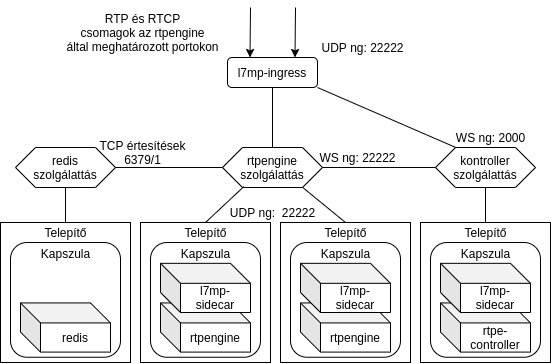
\includegraphics[width=1\textwidth, keepaspectratio]{figures/cluster.png}
	\caption{Kubernetes klaszter felépítése}
	\label{fig:clusterSetup}
\end{figure}

\subsection{Ingress}

Mint látszik a hálózatba való belépés az \texttt{l7mp-ingress} kapun történik, ahol 
kezdetben statikusan konfigurálva van egy figyelő, ami a dolgozó csomópont 22222 UDP 
portján vár minden az rtpengine-nek szánt vezérlőüzenetet. De látszik, hogy a kontroller 
szolgáltatás a 2000-s WebSocket porton várja az üzeneteket. Ezért az 
\texttt{l7mp-ingress} ezen figyelőjének tudnia kell UDP csomagokat WebSocket-re 
átalakítani. Ez az L7mp-nek köszönhetően nagyon egyszerűen megvalósítható volt ugyanis, 
elég csak egy UDP figyelőt létrehozni majd azt egy WebSocket L7mp klaszterekhez 
irányítani, aminek a végpontja a kontroller szolgáltatás. 

\subsection{Kontroller}

A munkám jelentős része ennek a kontrollernek az elkészítése volt, amit ebben a
fejezetben csak annyira ismertetek, hogy kiderüljön a szerepe a \ref{fig:clusterSetup}
ábrán szereplő architektúrában. Részletesen a \ref{sec:controller} fejezetben kerül 
kifejtésre. 

A kontroller a beérkező vezérlőüzeneteket automatikusan továbbítja az rtpengine 
szolgáltatásnak WebSocket-en keresztül. Mielőtt fojtatnám azzal, hogy a kontroller milyen 
feladatokat lát el fontos kifejteni a WebSocket protokoll szükségességét ebben az esetben.
Mivel minden WebSocket csomag rendelkezik egy HTTP-hez hasonló fejléccel így
lehet egyéni információkat küldeni fejlécekben. Ez az információ ebben az esetben a 
híváshoz tartozó  két azonosítót jelent. Az egyik a hívásazonosító míg a másik a hívásban 
résztvevő fél forrásazonosítója. Mivel ez a kettő információ fog szerepelni minden 
csomagban így elérhető az, hogy a vezérlő üzenetek mindig ugyanahhoz a kapszulához 
jussanak el.  Megakadályozva azt az esetet, amikor az \texttt{answer} és \texttt{offer} 
két különböző rtpengine kapszulához jut el, ami miatt nem tud kiépülni rendesen a hívás. 
Ennek elkerülésére a kontroller pótkocsijában kettő figyelőnek kell szerepelnie az egyik 
az \texttt{l7mp-ingress}-től várja a vezérlőüzeneteket és a másikon a helyi hálózatról 
várja azokat az üzeneteket, amiket el kell küldenie az rtpengine felé. 

De visszatérve arra, hogy a kontrollerre miért is van szükség. A kontrollernek két fő 
feladata van. Az első, hogy a hívásokhoz szükséges CRD-ket létrehozza és törölje, így az 
L7mp operátor tudni fogja, hogy milyen beállításokat kell alkalmaznia az L7mp proxy 
pótkocsikban. Aztán van a másik feladata, amivel a kimenő üzeneteket kell átírni annak 
megfelelően, hogy a dolgozó csomópont címe legyen benne és ne \texttt{127.0.0.1}, mert az 
rtpengine mindig ezt a címet fogja beletenni a módosított SDP üzenetekbe. 

\subsection{rtpengine}\label{sec:rtpengine}

Az rtpengine ebben az esetben teljesen ugyanazt a funkciót látja el, mint egy normális 
hívás esetében azzal a különbséggel, hogy képes redundánsan működni. Szóval, ha az 
egyiken létrejön egy hívás, akkor az létezni fog a másikon is és képes rögtön kezelni a 
beérkező forgalmat. Ezt oly módon teszi, hogy minden híváshoz létrehoz egy rekordot a 
Redis adatbázisban, ami keyspace-ket (kulcshelyeket) használ. Azért van szükség arra, 
hogy kulcshely tábla legyen használva az adatbázisban, mert erre fel lehet iratkozni. 
Szóval a két rtpengine kapszula feliratkozik ugyanarra a kulcshelyre, ahova mind a két 
kapszula fogja írni a beérkező hívásaikat. Tehát, ha az egyik kapott egy hívást az 
létrehoz egy rekordot az adott kulcshelyen, amiről a Redis értesíti a másik kapszulát és 
elküldi annak ezeket az információkat, ami majd létrehozza az adott hívást és kinyitja az 
hozzá szükséges portokat.  

De ez a funkció ebben a formában nem szerepel az rtpengine-ben. A hivatalos verzióban 
csak úgy működik, ha minden rtpengine példány látja egymást a hálózaton és már 
létrejöttükkor tudják egymás címét és, hogy melyik példány melyik kulcshelyet használja. 
Ez Kubernetes hálózatban nem túl szerencsés megoldás, mivel a kapszulák bármikor 
törlődhetnek és más címmel jöhetnek létre. Az általam használt megoldás az
rtpengine kódbázis egy nem hivatalos, experimentális módosításán alapul \cite{oded}. 
Lehetőséget adva az rtpengine példányok olyan módon történő skálázására, ami nem követeli 
meg a többi rtpengine címének pontos ismeretét. A megvalósítás azonban rendelkezik egy 
olyan problémával, hogy SRTP (Secure Real-time Transport Protocol) esetén nem minden 
hívást képes felépíteni az újonnan létrejött rtpengine. Ezáltal nem olvasztották be a fő 
kódbázisba, ezért nem tudom a hivatalos rtpengine-t használni.

Viszont itt még nem oldódott meg teljesen a probléma, ugyanis ez a verziója az 
rtpengine-nek csak skálázásra működött így, ha kettő példány fut egymás mellett, nevezzük 
őket \textbf{A}, \textbf{B}-nek. Akkor, ha \textbf{A}-hoz beérkezik egy hívás, erről 
értesül \textbf{B}, viszont nem nyitja ki hozzá a megfelelő portokat. Tehát, ha bármi 
történik \textbf{A}-val \textbf{B} nem tudja fogadni a hozzá beérkező forgalmat. Ennek a 
kiküszöbölése gyanánt egy kicsit módosítanom kell az rtpengine kódján, hogy mikor 
frissítés történik az adatbázisból, akkor portokat is nyisson ki. Ez egy elfogadható 
megoldásnak lehet tartani átlag esetben, viszont a Kubernetes világában ez a megoldás nem 
a legszebbek közé tartozik, mert nem követi a Kubernetes által diktált irányokat. A szép 
megoldás az lenne, ha a \textbf{B} példányon csak akkor nyílnának ki ezek a portok, ha 
\textbf{A} biztosan megszűnt. Ezt a későbbiek során lehet javítani.

A pótkocsik még nagyon fontosak ennél a résznél. Itt három fontos figyelő van, melyek 
közül kettő dinamikusan módosul.

\begin{enumerate}
	\item Van egy figyelő, ami WebSocket üzeneteket vár a 22222-s porton és ezeket 
	alakítja át UDP üzenetekre egy UDP L7mp klaszterrel, aminek a végpontja a 
	\texttt{127.0.0.1:22222} cím. Ezen a címen várja az rtpengine a vezérlőüzeneteket. 
	\item Induláskor statikusan kerül be egy üres figyelő a 19000-s portra, amire az RTP 
	csomagok fognak érkezni és bejutni az rtpengine által beállított portokra. Itt 
	felmerül a kérdés, hogy több hívás esetén hogyan kerülnek megkülönböztetésre a 
	hívásokhoz tartozó csomagok. Ezt az oldja meg, hogy az \texttt{l7mp-ingress} ezeket a 
	csomagokat mind JSONSocket protokollúra alakítja át, ami már rendelkezik fejléccel, 
	ami tartalmazza a hívás azonosítóját és a hívó címkéjét. Ezáltal dinamikusan hozzá 
	lehet adni szabályokat ehhez a figyelőhöz és az összes beérkező médiaforgalmat képes 
	jó irányba küldeni. 
	\item Lényegében ugyanazt a funkciót valósítja meg, mint az előző, azzal a 
	különbséggel, hogy ez a figyelő a 19001-s porton hallgat RTCP csomagokat. 
\end{enumerate}

\section{rtpengine kontroller}\label{sec:controller}

A kontrollernek két fő feladata van egy hívás felépítése során. Az egyik, hogy
a vezérlőprotokoll üzeneteit feldolgozza illetve továbbítsa az rtpengine
felé. A másik pedig a híváshoz szükséges L7mp beállításokat hivatott 
megvalósítani.

Ehhez készítettem egy python szkriptet, ami ezeket a feladatokat képes ellátni
különböző protokollokat támogatva. Azért a python lett választva a megvalósításhoz,
mert ezt a nyelvet viszonylag jól ismerem illetve nagyon jó Kubernetes 
támogatottsága van. Lehetővé téve azt, hogy a fejlesztés során gyorsan lehessen haladni.

Fontos megjegyezni, hogy a kontroller nem csak L7mp környezetben való használtra lett
tervezve, hanem Envoy-l is, így vannak olyan megvalósítások, amik csak Envoy
vagy L7mp környezetben nyernek értelmet. 

\subsection{Használata}

Mielőtt részleteiben kifejtésre kerülne a kontroller működése, szeretném bemutatni a
használatát.

A kontroller működéséhez biztosítani kell egy konfigurációs fájlt, amiben definiálva
van minden olyan paraméter, ami szerint szeretnénk, ha működne. Ezek a paraméterek
az alábbi felsorolásban olvashatóak.

\begin{itemize}
	\item \textbf{protocol}: Használt protokoll a vezérlőparancsok küldéséhez. Ez lehet
	udp, tcp és ws azaz WebSocket is.
	\item \textbf{rtpe\_address}: Az rtpengine szolgáltatás neve vagy IP címe. 
	\item \textbf{rtpe\_port}: A port, amin az rtpengine várja a beérkező parancsokat. 
	\item \textbf{envoy\_address}: Ha Envoy környezetben van használva akkor a menedzsment
	szolgáltatás neve vagy IP címe. 
	\item \textbf{envoy\_port}: Envoy menedzsment szolgáltatás portja. 
	\item \textbf{local\_address}: Lehet állítani, hogy az üzenetek küldése során milyen
	lokális címről küldje. Ez L7mp környezetben a \texttt{127.0.0.1} míg Envoy esetében 
	\texttt{0.0.0.0}.
	\item \textbf{local\_port}: Meghatározható, hogy a kimenő parancsok mely portról
	induljanak el. 
	\item \textbf{sidecar\_type}: Használt proxy típusa állítható be, ami lehet L7mp és 
	envoy is.
	\item \textbf{without\_jsonsocket}: A fejlesztés során több fajta architektúrát 
	kipróbáltam és ennek paraméternek a beállításával lehet váltani a létrehozandó L7mp 
	erőforrások között. 
	\item \textbf{ingress\_address}: A Kubernetes dolgozó csomópontjának az IP címe 
	adható meg. Azért van erre szükség, mert később ez a cím fog bekerülni a klienseknek 
	válaszolt SDP üzenetekbe. 
\end{itemize}

Ezt a konfigurációs fájlt érdemes létrehozni úgynevezett ConfigMap segítségével, amit 
fel lehet használni a kontroller kapszulájának leírása során. Egy ilyen ConfigMap-ben kis 
fájlokat lehet létrehozni és azokat hozzáadni különböző telepítő definíciókhoz. 

A \ref{lst:kubeSpec} kódrészletben látható, hogy Kubernetes-n belül ezt a konténert 
hogyan kell létrehozni és elindítani benne a kontrollert. 

\begin{lstlisting}[caption=Kubernetes konténer specifikációja, label=lst:kubeSpec]
...
spec:
  volumes:
    - name: controller-volume
      configMap:
        name: controller-config
  containers:
    - name: rtpe-controller
      image: vidarhun/rtpe-controller
      volumeMounts:
        - name: controller-volume
          mountPath: /app/config
      command: ["python"]
      args: ["controller.py", "-c", "config/config.conf", "-l", "debug"]
...
\end{lstlisting}

A \texttt{volumes} részben került betöltésre a \texttt{controller-config} ConfigMap, ami 
tartalmaz egy a kontroller számára megfelelő konfigurációt. Majd a 
\texttt{volumeMounts} részben kerül felcsatolásra a konténernek. Elérhetővé téve a 
\texttt{controller-config}-ban meghatározott fájlt az \texttt{/app/config} mappában a 
konténeren belül. Végül pedig a \texttt{command} és az \texttt{args} paraméterekkel indul 
el maga a kontroller, ahol \texttt{-c} argumentummal lehet a konfigurációs fájl elérését 
megadni és az \texttt{-l} argumentummal lehet állítani, hogy milyen szinten naplózzon a 
kontroller.

\subsection{Kontroller részei}

A kontroller fő részei közé tartozik az, hogy a Kubernetes API-val 
hogyan történik a kommunikáció, vezérlőprotokoll parancsainak megalkotása és
a beérkező üzenetek feldolgozása. 

\subsubsection{Kubernetes API}

Ahogy a használt eszközök bemutatása fejezetben is lehet olvasni a Kubernetes
klaszternek parancsokat a Kube API-n keresztül lehet adni. Ezért kellett egy olyan
módszert találni, amivel a kontroller képes kommunikálni a Kubernetes API-val 
egy kapszulából. Ehhez használtam egy olyan könyvtárat \cite{pythonKubeAPI}, amivel
könnyen megvalósítható az API-val való kommunikáció. Mindemellett nagyon jól
van dokumentálva ez a könyvtár, így viszonylag egyszerűen használható.

A könyvtár telepítése után inicializálni kell a kapcsolatot a Kubernetes 
API-val, amihez a \texttt{client} és \texttt{config} modult kell importálni
a Kubernetes könyvtárból. Majd a \texttt{config.load\_incluster\_config()}
hívással lehet inicializálni az API-val való kapcsolatot, így jelezve, hogy a
szkript egy Kubernetes klaszteren belül egy kapszulában fog futni. De ahhoz ez 
ténylegesen jól működjön ahhoz konfigurálni kell az RBAC-t (Role-based access control), 
amivel olyan jogokat lehet biztosítani, amikkel hozzálehet férni Kubernetes  
erőforrásokhoz. Szabályozni lehet ezzel azt is, hogy egy adott erőforráshoz  csak 
olvasási joggal rendelkezik a szkript így biztonságosabbá tehető a használata.

A kontrollerhez a \ref{lst:rbac} látható YAML definíció létrehozásával lehet olyan jogokat
adni, amikkel nagyjából bármilyen művelet eltud látni az L7mp által specifikált 
erőforrásokon.

\begin{lstlisting}[caption=RBAC létrehozása, label=lst:rbac]
apiVersion: rbac.authorization.k8s.io/v1
kind: ClusterRole
metadata:
  name: rtpe-controller
rules:
  - apiGroups: ["l7mp.io"]
    resources: ["virtualservices", "targets", "rules"]
    verbs: ["get", "list", "watch", "create", "update", "patch", "delete"]
---
apiVersion: rbac.authorization.k8s.io/v1
kind: ClusterRoleBinding
metadata:
  name: rtpe-controller
subjects:
  - kind: ServiceAccount
    name: default
    namespace: default
    roleRef:
      kind: ClusterRole
      name: rtpe-controller
      apiGroup: rbac.authorization.k8s.io
\end{lstlisting}

A \texttt{ClusterRole} segítségével lehet névtértől függetlenül jogokat biztosítani,
amik ebben az esetben az L7mp által specifikált egyéni erőforrásokra vonatkoznak. 
Ezeket az erőforrásokat az \texttt{apiGroups} illetve a \texttt{resources} listával
lehet megadni. Majd a \texttt{verbs} listában meghatározott műveletekre kap 
jogok a kontroller, így képes adott erőforrás állapotát lekérni, listázni, figyelni,
erőforrásokat létrehozni, frissíteni, kiegészíteni és törölni. 

Majd ezt követően a \texttt{ClusterRoleBidning} erőforrással lehet egy adott
felhasználóhoz hozzárendelni a létrehozott jogokat. Ebben az esetben az alapértelmezett
felhasználó kapja meg ezeket a jogokat tekintve, hogy a Kubernetesben csak ez az egy
felhasználó van definiálva. Végül a \texttt{roleRef}-ben lehet megadni, hogy mely
jogokat kapja meg a definiált felhasználó. 

Most, hogy már inicializálva van a Kubernetes API, létre kell hozni egy olyan 
API objektumot a kontrollerben, amivel egyéni erőforrás definíciókat lehet létrehozni
és törölni a Kubernetes klaszterben. Ezt a következő sor használatával lehet létrehozni: 
\texttt{api = client.CustomObjectsApi()}.

Most már szabadon lehet az L7mp objektumait létrehozni és törölni a kontrollerből is, 
ami az előzőleg létrehozott \texttt{api} objektum 
\texttt{create\_namespaced\_custom\_object()} illetve a 
\texttt{delete\_namespaced\_custom\_object()} segítségével valósítható meg. Az elsőnek 
említett függvény az alább felsorolt paramétereket várja.

\begin{itemize}
	\item \textbf{group}: A létrehozni kívánt erőforrás API címe.  
	\item \textbf{version}: A \textit{group}-ban definiált API verziója. 
	\item \textbf{namespace}: Melyik névtérben legyen létrehozva az erőforrás.
	\item \textbf{plural}: Az erőforrás típusának többesszáma. Ez az előzőleg definiált
	ClusterRole resources listájából valamelyik elem. 
	\item \textbf{body}: Egy YAML definíciót kell megadni python szótárként. 
\end{itemize}

Ezek közül a legfontosabb body, azaz a törzs, ahova mindig a híváshoz szükséges 
definíciókat kell megadni. Ahhoz, hogy kódban ne legyenek ezek a definíciók annyira 
beégetve, ahhoz ezeket a YAML fájlokat kiszerveztem egy mappába és, mikor használni vagy 
módosítani kell, akkor csak a szükséges fájlt beolvassa a kontroller és módosítja a 
szükséges mezőket.

Ha egy hívás beérkezik a kontrollerhez, akkor kettő virtuális szolgáltatás és kettő
szabály fog létrejönni. A szolgáltatások mindig az \texttt{l7mp-ingress}-n fognak 
beállítódni, ugyanis ezek nyitják ki a rtpengine által meghatározott portokat a kliensek 
számára a Kubernetes klaszteren. A két szabály pedig az rtpengine kapszulák melletti L7mp 
proxyban fog létrejönni, ahol a már előre definiált szabálylistához adódnak hozzá. 

Az így létrehozott erőforrásoknak a neveit tárolni kell, mivel a hívás vége után ezeket
a létrehozott erőforrásokat törölni kell mindig, ahhoz pedig szükséges az erőforrás 
neve. 

\subsubsection{Konfigurálás és naplózás}

A kontroller indítása után az első feladata az a kódnak, hogy beolvassa az indítás
során megadott argumentumokat és feldolgozza az konfigurációs fájlban megadott 
paramétereket. Az argumentumok beolvasását a \texttt{argparse} \cite{argparse} könyvár 
használatával oldottam meg, mivel könnyen használható és bővíthető. Lehetővé téve, hogy a
későbbiekben, ha több argumentum átadására van szükség nem lesz nagy feladat a 
megvalósítása. Másfelől a konfigurációs fájl feldolgozásához is létezik egy könyvtár, 
amit \texttt{configparser}-nek \cite{configparser} hívnak és a Microsoft Windows INI 
fájljaihoz hasonló konfigurációkat képes beolvasni. Beolvasás után feloldásra kerülnek az 
olyan paraméterek értékei, amik tartalmazhatnak tartomány neveket is. Erre azért van 
szükség, mert létrehozott foglalatokkal csak konkrét IP címekre lehet csomagokat küldeni. 
A beolvasott paraméterek egy globális szótár objektumba kerülnek, ami miatt ezek a 
paraméterek könnyedén elérhetőek lesznek bármelyik függvényből. Ezzel a fejlesztés nagy 
mértékben megkönnyebbül és átláthatóbb lesz a kód is.

A naplózás egy kulcsfontosságú része a kontrollernek, mivel fejlesztéskor vagy használata
során az \texttt{stdout}-ra kiírt események nagyban segítik a problémák keresését illetve 
azok megoldását. Naplózáshoz a \texttt{logging} \cite{logging} nevezetű könyvtárat 
használom, amiatt mert sok más könyvtár is ezt használja így, ha azok is valamit 
naplóznak, akkor az egyben látható lesz. Inicializálása során megadható, hogy milyen 
szinten naplózza az eseményeket és az is, hogy milyen formátumba. Ezért a kontroller egy 
naplóbejegyzése az \ref{lst:logging} látható módon néz ki, ami a másodpercre pontos 
időből, a naplózás szintjéből illetve magából az üzenetből áll.

\begin{lstlisting}[caption=Naplózás formátuma, label=lst:logging]
15:41:55 [INFO] Started!
15:41:55 [INFO] Configuration file loaded!
\end{lstlisting}

\subsubsection{Foglalatok létrehozása}

Mivel a kontroller három protokollt képes jelenleg támogatni ezért háromféle foglalatot 
kell tudnia használni. Név szerint az UDP, TCP, WebSocket protokollokat támogatják. 
Ezeknek a létrehozására mind van egy-egy függvény, ami képes a hozzájuk tartozó 
beállításokat beállítani és a megfelelő foglattal visszatérni, hogy azt több helyen 
lehessen használni.

A legegyszerűbb ebben az esetben az UDP foglalat megalkotása. Azért ez a legegyszerűbb,
mert ennél nem kell figyelembe venni a célját, mint a TCP esetében. Egy UDP foglalat 
létrehozáshoz szükség van a lokális címre és portra, amikhez a foglalatot hozzá kell 
kötni. A hozzákötés után, ha ezen a foglalaton keresztül történik csomagtovábbítás, 
akkor a megadott cím és port lesz a forrás cím és port. Emellett beállításra is
kerül egy időtúllépés paraméter is, ami 10 másodperc lesz. Ez azt jelenti, hogy
mikor a foglalat éppen csomagokat vár, akkor 10 másodpercig fog várni, majd generál 
egy kivételt és visszalép. Lehetőséget adva arra, hogy periodikusan lehessen
bizonyos feladatokat ellátni. 

Aztán van a TCP foglalat, aminél már figyelembe kell venni azt, hogy a WebSocket
protokollt használó kliens számára lesz gyártva vagy szimpla TCP kommunikációhoz 
használják. Ugyanis, ha önmagában kerül felhasználásra, akkor hozzáköti magát
az adott lokális címhez és porthoz és lényegében ugyan úgy kerül felhasználásra,
mint UDP esetben. Viszont, ha WebSocket kliens számára van létrehozva, akkor ezt
nem teszi meg, de ehelyett csatlakozik az rtpengine-hez az adott címen. Azt, hogy
miért van szükség a WebSocket számára egy TCP foglalatra azt a következő részben 
fejtem ki bővebben. De a csatlakozás az rtpengine-hez azért szükséges ebben az
esetben, mert másképp a kliens nem tudja TCP-nél jellemző kézfogás folyamatot
teljesíteni az rtpengine-l.

Végül pedig van a WebSocket verzió, amikor egy WebSocket foglalat kerül létrehozásra.
De ennek a létrehozására nem az általában használt python könyvtárat a \texttt{socket}-t
fogja használni, hanem a \texttt{websocket} \cite{websocket} könyvtárnak a 
\texttt{create\_connection()} függvényét. Ezzel a függvény egy olyan foglalattal tér 
vissza, aminél az elküldött üzenetek rendelkezni fognak a létrehozáskor beállított 
fejlécekkel. A \ref{lst:wssock} függvény az, ami a kontrolleren belül létrehozza a 
WebSocket foglalatot. 

\begin{lstlisting}[language=python, caption=WebSocket foglalat létrehozása, label=lst:wssock]
def create_ws_socket(sock, header):
    return create_connection(
        f'ws://{config["rtpe_address"]}:{config["rtpe_port"]}',
        subprotocols=["ng.rtpengine.com"],
        origin=config['local_address'],
        socket=sock,
        header=header
)
\end{lstlisting}

A következő listában sorrendben olvashatóak, hogy mely argumentum mit állít be és miért
pont azt.

\begin{itemize}
	\item Az rtpengine meghirdetett WebSocket URL-jét (Uniform Resource Locator) kapja 
	meg. Fontos, hogy ezt kapja, mivel az rtpengine egyszerre többféle protokollon 
	keresztül tud vezérlőparancsokat fogadni.
	\item Alprotokollokat is lehet használni WebSocket esetén, ami azért fontos, mert
	az rtpengine csak azokat a WebSocket csomagokat képes feldolgozni, amik rendelkeznek
	ezzel az \texttt{ng.rtpengine.com} alprotokollal.
	\item A forrás címet lehet beállítani az \texttt{origin} argumentummal. 
	\item Be lehet állítani azt, hogy a kapcsolat kiépítése során egyéni foglalatot
	használjon, így könnyen kontrollálható, hogy a foglalat milyen paraméterekkel 
	rendelkezzen. Ezért van szükség arra, hogy a TCP foglalat megalkotása során
	figyelembe vegyük azt, hogy WebSocket kliens számára hozzuk létre vagy csak úgy
	általánosan.
	\item Meg lehet adni egyéni fejléceket is, amikben bármi tárolható egy adott
	méretig. Ha létrejön egy hívás, akkor itt beállítódott hívás azonosítója alapján
	fogja a mellette lévő L7mp proxy eldönteni, hogy mely rtpengine kapszula kapja
	meg az üzeneteket.
\end{itemize}

\subsubsection{Erőforrások létrehozása és törlése}

Arról, hogy az erőforrások létrehozása illetve törlése mikor történik a feldolgozás
fejezetben lesz szó. Ebben arról lesz, hogy hogyan működnek.

Mikor elindul a kontroller, akkor már a kezdetekkor van egy \texttt{kubernetes\_apis}
lista, ami tartalmazza az összes Kubernetes API kliens objektumot. Ezáltal mindig van egy
pontos képe a kontrollernek arról, hogy milyen paraméterekkel lettek erőforrások 
létrehozva a működése során. Szóval egy új hívás esetén kettő új API kliens objektum 
fog bekerülni ebbe a listába, egy hívó fél adataival és egy a hívott fél adataival 
és törlésnél ez a kettő kerül törlésre a hívásazonosító alapján. 

Egy erőforrás létrehozása során elsőnek ebben a listában kell ellenőrizni azt, hogy
ilyen hívásazonosítóval már létezik-e erőforrás, ha nem létezik csak akkor lehet 
létrehozni. Erre azért van szükség, mert a Kamailio rendelkezik egy válaszidővel, ami ha 
lejár akkor az utoljára kiküldött üzenetet megismétli. De ebben az esetben könnyen 
előfordulhat, hogy később küldi vissza a kontroller az üzenetet, mint ez az időkeret és 
ilyenkor a duplikáltan küldött üzeneteket elveti a kontroller.

Ezután egy \texttt{query} üzenetet kell küldeni az rtpengine felé, ugyanis az 
\texttt{offer} és \texttt{answer} üzenetekre kapott válaszban nem biztos, hogy ugyan
az a port lesz lefoglalva. De a \texttt{query} üzenettel ez kiküszöbölhető, mert az 
erre adott válaszban mindig a megfelelő portok fognak szerepelni. A portokra azért van
szükség, mert az API kliens objektumok által létrehozott erőforrásokban ezek használva
vannak. A \ref{lst:kubeAPI} látható, hogy egy API kliens objektum miként kerül 
létrehozásra.

\begin{lstlisting}[language=python, caption=Kubernetes API kliens objektum létrehozása, label=lst:kubeAPI]
kubernetes_apis.append(
    Client(
        call_id=call_id,
        tag=tag,
        local_ip=address,
        local_rtp_port=client_port,
        local_rtcp_port=client_port + 1,
        remote_rtp_port=remote_port,
        remote_rtcp_port=remote_port + 1,
        without_jsonsocket=config['without_jsonsocket'],
        ws=ws
    )
)
\end{lstlisting}

Az első argumentummal lehet meghatározni a hívás azonosítóját és a másodikkal a félhez
tartozó címkét, ami lehet \texttt{from-tag} és \texttt{to-tag} is. Majd ezután jön a
klienshez tartozó cím, RTP és RTCP port. Aztán az rtpengine által a híváshoz lefoglalt
RTP és RTCP port, végül pedig a \texttt{without\_jsonsocket} és \texttt{ws} 
argumentumokkal lehet még erőforrásokra vonatkozó paramétereket megadni.

Ha ez a konstruktor sikeresen lefutott, akkor az azt jelenti, hogy a Kubernetes 
klaszterben létrejött minden szükséges erőforrás és adott minden a média forgalom 
kezeléséhez.

A törlés ezzel szemben nagyon egyszerűen úgy történik, hogy a hívásazonosító alapján
\texttt{kubernetes\_apis} listából meghívjuk az objektum \texttt{delete\_resources()}
függvényét, ami az adott híváshoz kapcsolódó összes erőforrást törölni fogja.

\subsubsection{Parancsok feldolgozása}

A parancsok feldolgozása kétféle módon történhet, lehet az átlagos foglalatokkal, ami 
a TCP és UDP csomagok kezelését jelenti illetve lehet a WebSocket protokoll segítéségével 
is. Az előzőleg említett feldolgozás lehetővé teszi, hogy mind TCP és UDP
foglalatok használatával működjön, mert ezek a foglalatok küldés és fogadás szempontjából
teljesen ugyanazokat a függvényeket valósítják meg.

Az említett eljáráshoz tartozó függvény két foglalatot vár el argumentumként, amik közül 
a \texttt{sock} az a foglalat lesz, amelyik a kliensektől várja a bejövő forgalmat és az 
\texttt{rtpe\_sock} lesz, amelyen keresztül kommunikálni fog a kontroller az 
rtpnengine-el. Szóval a \texttt{sock}-n beérkező adat tárolásra kerül abban a formában, 
amelyben érkezik szóval egy egyszerű karakterláncként és a feldolgozott verziója is, 
amikor karakterlánc bencode által kódolt része feloldásra és szótárba írásra kerül. Ez a 
feldolgozott változat hasznos akkor, amikor az erőforrásokat kell létrehozni, míg a nyers 
beérkezett üzenet továbbküldésre kerül az rtpengine felé, hiszen azon nem kell 
változtatni semmilyen paramétert.

Ha az rtpengine válaszolt az adott parancsra és ez a parancs nem tartalmazott semmilyen 
SDP üzenetet, akkor egyszerűen visszaküldésre kerül a kliensnek. De ha a parancs egy 
\texttt{offer} vagy \texttt{answer} üzenet volt, akkor az rtpengine által adott válaszban 
szereplő SDP üzenetben módosítani kell a kapcsolat kiépítéséhez szükséges paraméterben 
szereplő IP címet. Ugyanis ez a cím minden esetben \texttt{127.0.0.1} lesz, ami nem jó az 
olyan SIP klienseknek, mint a Linphone. A szóban forgó címet kell lecserélni a dolgozó 
csomópont IP címére. De az rtpengine válasza után még vizsgálni kell azt is, hogy milyen 
parancs érkezett be a kontrollerhez. Ha egy \texttt{delete} üzenet érkezett, akkor a 
benne szereplő hívásazonosítóhoz tartozó Kubernetes erőforrásokat mindenképpen törölni 
kell, hogy véletlenül sem maradjon nyitva olyan port a Kubernetes klaszteren, ami nincs 
használatban. A másik ilyen fontos üzenet az \texttt{answer}. Azért kell az ilyen 
paranccsal rendelkező üzenetekre jobban figyelni, mint az \texttt{offer}-re, mert csak 
ennek a megékezése után lehet a megfelelő erőforrások

\section{Kliens}

Ahhoz, hogy az előzőleg tárgyalt rendszert érdemben lehessen tesztelni írnom kellett egy 
saját alkalmazást, ami képes volt adott számú médiaforgalmat generálni, de tud 
kommunikálni az rtpengine-l is. Szóval egyben a SIP klienst és szervert is megvalósítja.

A kliens felépítése nagyon hasonlóan néz ki, mint a kontrolleré, ami azt eredményezi, 
hogy képesnek kell lennie  TCP, UDP és WebSocket protokollokon keresztül kommunikálni az 
rtpengine-l. Viszont a klienshez nem érkeznek be vezérlőparancsok, hanem a kliens gyártja 
ezeket, így a kliensnek tudnia kell az összes rtpengine által támogatott vezérlőparancsot 
megalkotnia bizonyos paraméterekkel. Ezen felül tudnia kell médiaforgalmat is generálni, 
amihez jelenleg két fajta megoldás létezik. Használható az FFmpeg és az rtpsend is arra, 
hogy ezt a forgalmat legenerálja, viszont mind a kettőnek megvan az előnye és a hátránya 
is. 

Ebben a fejezetben kifejtésre kerül a kliensben használt külső alkalmazások működése és 
célja, a kliens használata és annak felépítése. 

\subsection{FFmpeg \& rtpsend}

\subsubsection{FFmpeg}

Elsőnek az FFmpeg-t szeretném bemutatni, mert ezt az eszközt többen ismerhetik,
mint az rtpsend-t. 

Az FFmpeg \cite{ffmpeg} egy nyílt forráskódú szoftver, amely különböző könyvtárak 
felhasználásával képes videó, hang és egyéb multimédiás adatfolyamok kezelésére. Lehetővé 
téve olyan feladatok ellátását, mint kódolás, dekódolás, transzformálás és adatfolyam 
sugárázása. Viszont rendelkezik különböző hátrányokkal, amik nem elhanyagolhatóak a teszt 
szempontjából.

Az első ilyen probléma vele, hogy az erőforrás igénye nagyon magas tud lenni 
annak függvényében, hogy mennyire komplex feladatot lát el. Ez alapesetben nem lenne
probléma, viszont ebben a környezetben sok egymás mellett futó FFmpeg végez majd
komplex feladatot, amihez így sok erőforrás szükséges.

A második probléma, hogy a sugárzott RTP folyamot nem lehet eléggé testre szabni, 
amennyire szükséges lenne. Például a csomagokban lévő adat nem mindig lesz 
ugyanakkora méretű, ami a mérési eredményeket könnyen torzítani fogja, hiszen 
minden médiafolyam rendelkezik egy bizonyos kódolással, amihez megvan határozva, hogy
milyen méretű csomagok szükségesek.

Végül a legnagyobb probléma, ami előjön az FFmpeg és rtpsend esetében is, hogy nem
tudnak RTCP fogadó jelentést gyártani, ami miatt a hívás minősége nem monitorozható 
megfelelően. Ez a probléma úgy lett kiküszöbölve, hogy rtpsend vagy FFmpeg gyárt
egy adott mennyiségű háttérforgalmat és két Linphone kliens segítségével elindításra 
kerül mellettük egy teljes értékű hívás.  Lehetővé téve a rendszer által nyújtott minőség 
mérését adott háttérforgalom mellett. 

Az \ref{lst:FFmpeg} parancs szükséges ahhoz, hogy egy \texttt{wav} fájlt sikeresen 
lehessen sugározni RTP segítségével az rtpengine számára, így a híváshoz szükséges 
adatfolyamot lehet szimulálni. 

\begin{lstlisting}[caption=FFmpeg RTP folyam indtása, label=lst:FFmpeg]
ffmpeg -re -i audio.wav -ar 8000 -ac 1 -acodec pcm_mulaw \\
-f rtp 'rtp://127.0.0.1:23000?localrtpport=2000'
\end{lstlisting}

Ez a sor az \texttt{audio.wav} fájlt fogja a lokális hálózaton lévő rtpengine 23000-s
portjára küldeni a 2000-s portról \texttt{PCMU} kódolással. A következő felsorolás 
tartalmazza részletesen, hogy a paraméterei mit csinálnak.

\begin{itemize}
	\item \textbf{-re -i}: Natív képkockasebességgel való beolvasást tesz lehetővé, 
	így lehet szimulálni egy élő forrást, például egy mikrofont. Emellett lelassítja
	a fájl olvasásának sebességet annyira, hogy hasonlítson az a valós idejű
	adatbeolvasáshoz, ugyanis alapértelmezetten olyan gyorsan olvassa az FFmpeg a
	fájlokat amilyen gyorsan csak tudja és így gyorsabban lesz beolvasva a fájl,
	mint a fájl időtartama. 
	\item \textbf{-ar}: Beállítja a mintavételezési periódust, ami itt \texttt{8000 Hz}, 
	ami azt jelenti, hogy másodpercenként 8000 mintát vesz a forrásból. 
	\item \textbf{ac}: Beállítja a használt hangcsatornák számát.
	\item \textbf{-acodec}: Megadja, hogy milyen hangkódolást használjon. Ebben az 
	esetben PCM u-law alapú kódolás történik.
	\item \textbf{-f}: A kimenti fájl formátumát lehet megadni, de ebben az esetben
	nem egy fájl, hanem egy cím van megadva így a hálózaton RTP csomagokban fogja 
	küldeni a kódolt hanganyagot. Ha jobban megnézzük, akkor ez a cím két részből áll,
	ahol az első határozza meg azt, hogy hova küldje a csomagokat. Ez a 
	\texttt{127.0.0.1:23000} az rtpengine címe és a híváshoz meghatározott egyik RTP
	port. Míg a második rész a \texttt{localrtpport}, amivel meghatározható, hogy
	mely portról küldje ezeket a csomagokat.
\end{itemize}

\subsubsection{rtpsend}

Az rtpsend \cite{rtpsend} teljesen eltér az FFmpeg-től, hiszen itt nincs semmilyen hang 
vagy videó feldolgozás, átalakítás vagy bármi más. Itt egyszerűen csak egy RTP folyam 
visszajátszása történik, amit az \texttt{rtpdump} eszközzel lehet felvenni. Ez a két 
szoftver egy eszköztárba tartozik, aminek a neve \texttt{rtptools}, amit Henning 
Schulzrinne alkotott meg, aki a Columbia Egyetem oktatója.

Az rtpsend használatához elsőnek rögzíteni kell egy a híváshoz tartozó RTP folyamot az 
rtpdump paranccsal, ami úgy működik, hogy meg kell adni egy címet, amin az RTP csomagokat 
elkapja és ezeket alakítja át egy olyan formátumba, amit később az \texttt{rtpsend}-l újra
lehet alkotni. Abból a szempontból előnyös, hogy az rtpengine-nek a médiaformátum
átalakítását jól lehet vele tesztelni, mert fel lehet venni két különböző kódolású
hívást és azokat lejátszani egy szimulált híváson belül.

A lejátszáshoz ez a parancs lesz használva: 

\begin{lstlisting}[caption=RTP folyam generálásda rtpsend segítségével, label=lst:rtpsend]
rtpsend -l -s 3002 -f dump.rtp 127.0.0.1/23000
\end{lstlisting}

Ezzel azt az utasítást adjuk ki, hogy folyamatos ismétléssel küldje el a 
\texttt{dump.rtp} fájlt a \texttt{127.0.0.1:3002} címről a \texttt{127.0.0.1:23000}
címre, amin az rtpengine várja az egyik oldaltól a médiafolyamot.

\subsubsection{Linphone}

A Linphone egy ingyenes és nyílt forráskódú VoIP kliens alkalmazás, amivel hang- és 
videóhívásokat lehet lebonyolítani. Teljes mértékben SIP alapú kommunikációt használ és 
megadható egyéni SIP szerver is, amihez kommunikálhat, de igény és regisztráció esetén
használható az általuk nyújtott SIP szerver is. 

Hasznos funkciói közé tartozik a hang és videó kódolásának változtatási lehetősége, ami
lehetővé teszi, hogy mely kódolásokat szeretné a felhasználó használni hívás során.
Ezenfelül a parancssoros verziója képes előre rögzített \texttt{wav} fájlt lejátszani
a hívásban résztvevő feleknek. Az utóbbi funkciója a mérések folyamán rendkívül 
hasznosnak bizonyult, hiszen nem kellett megoldást találni arra, hogy virtuális gépek 
hangkártyájára miképp juttassak bármiféle hangot. 

\subsection{Felépítés}

A kliens felépítése nagyon hasonló, mint a kontrolleré és ez látszik abban is, hogy
ugyan azokat a könyvtárakat használja naplózáshoz, konfiguráció beolvasásához és
argumentumok átadására. Viszont a konfigurációs fájlban más paramétereket lehet 
beállítani. A következő felsorolásban fejtem, hogy mely paraméter milyen értékeket 
vehet fel és mi történik ezek használata során. 

\begin{itemize}
	\item \textbf{local\_address}: Meglehet adni, hogy milyen címről küldje
	ki a vezérlőparancsokat.
	\item \textbf{protocol}: Megadja, hogy milyen protokollt használjon a kliens az
	vezérlőparancsok küldésére. Ez lehet udp, tcp, ws azaz WebSocket.
	\item \textbf{rtpe\_address}: Az rtpengine címe. 
	\item \textbf{rtpe\_port}:Az rtpengine portja.
	\item \textbf{ping}: Ha csak azt akarjuk a klienssel ellenőrizni, hogy az rtpengine
	elérhető, akkor lehet küldeni egy szimpla \texttt{ping} üzenet. Ha visszajön egy
	\textit{pong} az rtpengine elérhető. Ha ennek a mezőnek az értéke yes, akkor 
	az előzőleg leírt megtörténik és vége a kliens futásának. 
	\item \textbf{number\_of\_calls}: A generálni kívánt hívások számát lehet megadni. 
	\item \textbf{send\_method}: Megadhatjuk, hogy FFmpeg vagy rtpsend segítségével
	generáljon médiaforgalmat a kliens.
	\item \textbf{wav\_location}: Ha FFmpeg lett beállítva a \texttt{send\_method} 
	paraméternél, akkor az ehhez szükséges wav hangfájl elérési útvonala adható meg.
	\item \textbf{rtp\_dump\_location}: Ha rtpsend lett beállítva a 
	\texttt{send\_method} paraméternél, akkor az ehhez szükséges rtp fájl elérési 
	útvonala adható meg.
\end{itemize}

Indításánál ugyanúgy a konfigurációs fájlt és a naplózás szintjét lehet beállítani,
mint a kontrollernél. 

A kontrollerhez hasonlóan működik még a foglalatok kezelése is. Szóval az UDP és TCP 
protokoll kezelése az teljesen ugyan az, de a WebSocket estében nincs szerver 
implementálva csak a kliens. 

\subsubsection{Médiaforgalom generálása}

Ahogy az előzőekben ki lett fejtve, a médiaforgalom generálására két eszközt 
használ a kontroller az rtpsend-t és az FFmpeg-t. Viszont ezekből tetszőleges
számút kell tudni elindítani attól függően, hogy hány párhuzamos hívást kell 
a kliensnek indítania.

Első próbálkozásnál a szálkezeléssel próbálkoztam, de hamar rá kellett jönnöm,
hogy az csak abban az esetben hasznos, ha python kódot kell konkurensen 
használni. Ezért átváltottam a \texttt{subprocess} \cite{subprocess} modulra, amivel külső alkalmazásokat lehet párhuzamosan használni.

Ahhoz, hogy ezzel a modullal létre lehessen hozni egy folyamatot, ahhoz a \texttt{Popen}
konstruktort kell használni, amiben az elindítani kívánt folyamat argumentumait lehet
megadni egy listaként. Mivel egy ilyen módon létrehozott objektum csak egyetlen 
folyamatot képes elindítani, ezért több ilyen objektumot kell létrehozni más 
paraméterekkel. Ezért az FFmpeg és az rtpsend esetében is meg kell találni azokat a 
részeket, amik minden hívásnál változnak és ezek szerint létrehozni ezeket az 
objektumokat. Az FFmpeg esetében elég volt a rtpengine címét és a híváshoz lefoglalt 
portját megadni. Ezeket a címeket egy listába rendezve majd a listát iterálva ellehet 
indítani hívásonként kettő FFmpeg folyamatot. Az rtpsend esetében is ugyanez a felállás, 
viszont ott a forrás és a cél port két különböző paraméterben szerepel. Ehhez már nem egy 
listát, hanem egy szótárat használtam, ahol az rtpengine címe volt a kulcs és a forrás 
port volt a hozzárendelt érték.

\subsubsection{Hívások generálása}

A hívás generálás során biztosítani kell azt, hogy legyen megfelelő mennyiségű port
nyitva médiaforgalomhoz és mielőtt a médiaforgalom elindul meg kell teremteni a hívást
magán az rtpengine szerveren. Az rtpengine-n híváskiépítéshez szükség van egy 
\texttt{offer} és \texttt{answer} üzenetpárosra.

Viszont mielőtt még ezek az üzenetek megalkotásra és elküldésre kerülnek azelőtt
a hozzájuk tartozó SDP üzeneteket kell megalkotni. Ezt egy sablon alapján készíti el 
a kliens, amiben módosítás során csak a munkamenet azonosító helyére kerül
mindig egy véletlenszerű szám és a kapcsolódást leíró paraméter kapja meg a lokális 
címet azaz a hívó félét. Ha ez megtörtént azután már ellehet küldeni elsőnek az 
\texttt{offer}-t majd az \texttt{answer}-t. Mind a két üzenet ugyanazzal a 
hívásazonosítóval és \texttt{from-tag}-l rendelkeznek, viszont az \texttt{answer} 
esetében meg kell adni egy \texttt{to-tag}-t is.

Az így megalkotott hívásról információk kerülnek tárolásra egy listában, ami szükséges
a hívások törléshez. Mert ha vége az adott folyamatoknak, attól még az rtpengine szerveren
él a hívás, csak nem érkezik be hozzá semmilyen adat. Ezek a hívások adott inaktivitás után automatikusan törlésre kerülnek, viszont abban az esetben, ha rövid időn 
belül új tesztet kell elindítani, akkor összeakadhatnak a portok és az azonosítók, így a 
kontroller olyan esetben, amikor a hívás megszakad küld egy \texttt{delete} 
vezérlőüzenetet az rtpengine felé hívásonként a hozzájuk tartozó azonosítókkal.

%%----------------------------------------------------------------------------   
\chapter{Architektúra}
%----------------------------------------------------------------------------

A Kubernetes architektúra tervezése során a fő szempont az volt, hogy teljes
mértékben úgy nézzen ki kívülről, mintha egy szimpla rtpengine lenne. De 
mögötte egy mikroszolgáltatásokból álló alkalmazás legyen, mely képes
az benne rejlő rtpengine-t megfelelően konfigurálni.

Ezt a fürtöt a BME által szolgáltatott szervereken építettem ki, mi szám szerint
4 szervert tartalmaz melyek az alábbi elrendezésben vannak összekötve.

\begin{figure}[!ht]
	\centering
	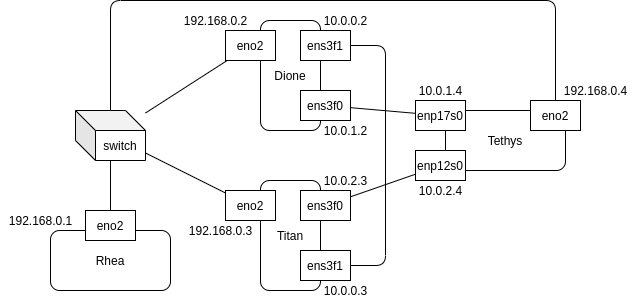
\includegraphics[width=1\textwidth, keepaspectratio]{figures/servers.png}
	\caption{Szerverek összeköttetése}
	\label{fig:servers}
\end{figure}

Az ábrán szereplő szervereket kettő részre lehet szétbontani, ahol az egyik
konkrétan a Kubernetes fürt a másik pedig a forgalom generálására használatos.
Az előbbibe tartozik a Rhea, mint mester csomópont és dolgozó csomópontok közé 
a Dione és a Titan. Majd értelemszerűen az utóbbiba tartozik a Tethys. 

A szerverek között a kapcsolatot a vonalakkal jeleztem, melyek, mint látszik
sok esetben direkt összeköttetésben vannak egymással. Ez azért van, mert ezek
az interfészek 40 gigabitesek és az egyetemen nem állt rendelkezésre ilyen 
sebességű switch. Ezáltal a Kubernetes fürt telepítése során különös figyelmet
kellett szentelni annak, hogy ezek az interfészek helyesen legyenek felkonfigurálva.

De, mint látszik a hálózatban szerepel egy switch, amibe az eno2 interfészek vannak
becsatlakoztatva. Ezek az interfészek 1 gigabites sebességgel rendelkeznek, amik
a sok nagy sebességű forgalmat nem képes kiszolgálni, viszont még így is hasznosak
a hálózat szempontjából. Mivel a telepített Kubernetes fürt vezérlő- és adatsíkja
ezen a két összeköttetésen osztozik. Szóval a lassabb interfészeken kommunikál az
API szerver és a kubelet, míg a kube-proxy a nagy sebességű hálózati kártyákat 
használja. Így lehetett egy olyan magas határt szabni a lehetséges forgalom
sebességének, amibe nehéz beleütközni. 

Ahhoz, hogy az előzőleg leírt hálózat elkülönítés működjön a Kuberspray programot 
használtam, mert ennél könnyedén lehetett a telepítés során kettő különböző interfészt
beállítani. A kuberspray \cite{kubespray} programmal Kubernetes fürtöket lehet telepíteni szimplán
szerverekre. A különlegessége az, hogy Ansible-t használ erre a célra. Szóval elég
a mester szerver számára lehetővé tenni, hogy működjön az ssh a többi szerverrel és
egyetlen konfigurációs fájl indításával képes minden szükséges szoftvert feltelepíteni
és azokat beállítani. Az Ansible \cite{ansible} nagyjából bármilyen folyamatot tud automatizálni a
szerverek között. 

\section{Kubernetes architektúra}

A címben említett architektúra írja le, hogy a fürtön belül milyen Kubernetes
erőforrások találhatóak meg és azok, hogyan vannak egymással összekötve. A következő
ábrát kifejtve lehet ezt legjobban elmagyarázni. Fontos megjegyezni, hogy erre 
a rengeteg átalakításra azért van szükség, mert a Kamailio legfrissebb
stabil verziója nem tud WebSocket-n keresztül vezérlőcsomagokat küldeni és az rtpengine-nek
az a verziója, amivel a Redis-t ilyen módon lehet használni nem támogatja szintúgy
a WebSocket-t. Viszont szükség van a WebSocket-re, ami a későbbiekben kifejtésre kerül.

\begin{figure}[!ht]
	\centering
	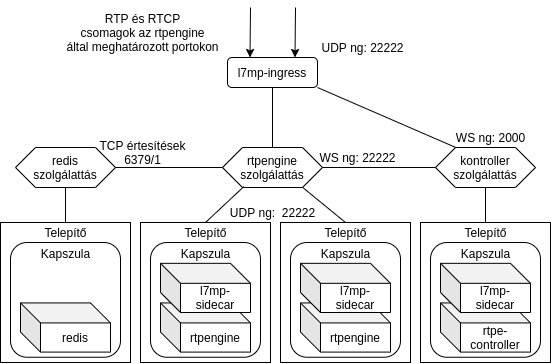
\includegraphics[width=1\textwidth, keepaspectratio]{figures/cluster.png}
	\caption{Fürt felépítése}
	\label{fig:HVSpaces}
\end{figure}

\subsection{Ingress}

Mint látszik a hálózatba való belépés az l7mp-ingress kapun történik, ahol kezdetben
statikusan konfigurálva van egy figyelő, ami a dolgozó csomópont 22222 UDP portján
vár minden az rtpengine-nek szánt vezérlőüzenetet. De látszik, hogy a kontroller szolgáltatás
a 2000-s WebSocket porton várja az üzeneteket. Ezért az l7mp-ingress ezen figyelőjének 
tudnia kell UDP csomagokat WebSocket-re átalakítani. Ez az L7mp-nek köszönhetően nagyon
egyszerűen megvalósítható volt ugyanis, elég csak egy UDP figyelőt létrehozni majd azt 
egy WebSocket fürthöz irányítani, aminek a végpontja a kontroller szolgáltatás. 


\subsection{Kontroller}
A kontroller a beérkező vezérlőüzeneteket automatikusan továbbítja az rtpengine 
szolgáltatásnak WebSocket-n keresztül. Mielőtt fojtatnám azzal, hogy a kontroller milyen 
feladatokat lát el fontos kifejteni a WebSocket protokoll szükségességét ebben az esetben.
Mivel minden WebSocket-nek  csomag rendelkezik egy HTTP-hez hasonló fejléccel így
lehet egyéni információkat küldeni fejlécekben. Ez az információ ebben az esetben a híváshoz
tartozó  két azonosítót jelent. Az egyik a hívásazonosító míg a másik a hívásban résztvevő
fél forrásazonosítója. Mivel ez a kettő információ fog szerepelni minden csomagban így elérhető az,
hogy a vezérlő üzenetek mindig ugyanahhoz a kapszulához jussanak el. Így elkerülhető az
az eset, hogy mondjuk egy answer és egy offer üzenet kettő különböző rtpengine kapszulához
jusson el. Így a kontroller pótkocsijában kettő figyelőnek kell szerepelnie, az egyik
az amin az l7mp-ingress-től várja a vezérlőüzeneteket és a másik, amin a helyi hálózatról
várja azokat az üzeneteket, amiket el kell küldenie az rtpengine felé. 

De visszatérve arra, hogy a kontrollerre miért is van szükség. A kontrollernek két fő feladata
van. Az első, hogy a hívásokhoz szükséges CRD-ket létrehozza és törölje, így az operátor tudni fogja,
hogy milyen beállításokat kell alkalmaznia az L7mp proxy pótkocsikban. Aztán van a másik feladata,
amivel a kimenő üzeneteket kell átírni annak megfelelően, hogy a dolgozó csomópont
címe legyen benne és ne 127.0.0.1, mert az rtpengine mindig ezt a címet fogja beletenni
a módosított SDP üzenetekbe. 

\subsection{rtpengine}

Az rtpengine ebben az esetben teljesen ugyanazt a funkciót látja el, mint egy normális hívás
esetében azzal a különbséggel, hogy képes redundánsan működni. Szóval, ha az egyiken létrejön
egy hívás, akkor az létezni fog a másikon is és képes rögtön kezelni a beérkező forgalmat. Ezt
oly módon teszi, hogy minden híváshoz létrehoz egy rekordot a Redis adatbázisban, ami 
keyspace-ket (kulcshelyeket) használ. Azért van szükség arra, hogy kulcshely tábla legyen
használva az adatbázisban, mert erre fellehet iratkozni. Szóval a két rtpengine kapszula
feliratkozik ugyanarra a kulcshelyre, ahova mind a két kapszula fogja írni a beérkező hívásaikat.
Így, ha az egyik kapott egy hívást az létrehoz egy rekordot az adott kulcshelyen, amiről a 
Redis értesíti a másik kapszulát és elküldi annak ezeket az információkat, ami majd létrehozza
az adott hívást és kinyitja az hozzá szükséges portokat.  

De ez a funkció ebben a formában nem szerepel az rtpengine-ben. A hivatalos verzióban csak úgy 
működik, ha minden rtpengine példány látja egymást a hálózaton és már létrejöttükkor tudják
egymás címét és, hogy melyik példány melyik kulcshelyet használja. Ez Kubernetes hálózatban
nem túl szerencsés megoldás, mivel a kapszulák bármikor törlődhetnek és más címmel jöhetnek 
létre. Ezért kellett találni egy megoldást, amit egy bizony Oded Arbel pull request-je (ajánlása)
\cite{oded} jelentett. Ugyanis szerette volna, ha lehet skálázni az rtpengine példányokat anélkül, hogy 
tudnánk a létező többinek a címét is. Ezt majdnem teljesen jól megoldotta, viszont egy olyan 
problémába ütközött, hogy SRTP (Secure Real-time Transport Protocol) esetén nem minden hívást képes 
felépíteni az újonnan létrejött rtpengine. Így nem olvasztották be a fő kódbázisba, ezért nem tudom a 
hivatalos rtpengine-t használni.

Viszont itt még nem oldódott meg teljesen a probléma, ugyanis ez a verziója az rtpengine-nek csak
skálázásra működött így, ha kettő példány fut egymás mellett, nevezzük őket \textbf{A}, 
\textbf{B}-nek. Akkor, ha \textbf{A}-hoz beérkezik egy hívás, erről értesül \textbf{B}, viszont nem
nyitja ki hozzá a megfelelő portokat. Így, ha bármi történik \textbf{A}-val \textbf{B} nem tudja
fogadni a hozzá beérkező forgalmat. Ennek a kiküszöbölése gyanánt egy kicsit módosítanom 
kell az rtpengine kódján, hogy mikor frissítés történik az adatbázisból, akkor portokat is nyisson ki.
Ez egy elfogadható megoldásnak lehet tartani átlag esetben, viszont a Kubernetes világában
ez a megoldás nem a legszebbek közé tartozik, mert nem követi a Kubernetes által diktált
irányokat. A szép megoldás az lenne, ha a \textbf{B} példányon csak akkor nyílnának ki ezek a 
portok, ha \textbf{A} biztosan megszűnt. Ezt a későbbiek során lehet javítani. \\

A pótkocsik még nagyon fontosak ennél a résznél. Itt három fontos figyelő van, melyek közül
kettő dinamikusan módosul.

\begin{enumerate}
	\item Van egy figyelő, ami WebSocket üzeneteket vár a 22222-s porton és ezeket alakítja át
	UDP üzenetekre egy UDP fürttel, aminek a végpontja a 127.0.0.1:22222 cím. Ezen a címen várja
	az rtpengine a vezérlőüzeneteket. 
	\item Induláskor statikusan kerül be egy üres figyelő a 19000-s portra, amire az RTP csomagok
	fognak érkezni és bejutni az rtpengine által beállított portokra. Itt felmerül a kérdés, hogy 
	több hívás esetén hogyan kerülnek megkülönböztetésre a hívásokhoz tartozó csomagok. Ezt az
	oldja meg, hogy az l7mp-ingress ezeket a csomagokat mind JSONSocket-re alakítja át, ami már 
	rendelkezik fejléccel, ami tartalmazza a hívás azonosítóját és a hívó címkéjét. Így dinamikusan
	hozzá lehet adni szabályokat ehhez a figyelőhöz és az összes beérkező médiaforgalmat képes jó
	irányba küldeni. 
	\item Lényegében ugyanazt a funkciót valósítja meg, mint az előző, azzal a különbséggel, hogy
	ez a figyelő a 19001-s porton hallgat RTCP csomagokat. 
\end{enumerate}


 
%%----------------------------------------------------------------------------   
\chapter{Kontroller}
%----------------------------------------------------------------------------

A kontrollernek két fő feladata van egy hívás felépítése során. Az egyik, hogy
a vezérlőprotokoll üzeneteit feldolgozza illetve továbbítsa az rtpengine
felé. A másik pedig a híváshoz szükséges l7mp beállításokat hivatott 
megvalósítani.

Ehhez készítettem egy python szkriptet, ami ezeket a feladatokat képes ellátni
különböző protokollokat támogatva. Azért a python lett választva a megvalósításhoz,
mert ezt a nyelvet viszonylag jól ismerem illetve nagyon jó Kubernetes 
támogatottsága van. Így könnyen és gyorsan lehetett haladni az írásával. \\

Fontos megjegyezni, hogy a kontroller nem csak l7mp környezetben való használtra lett
tervezve, hanem Envoy-l is. Így vannak olyan megvalósítások, amik csak Envoy
vagy l7mp környezetben nyernek értelmet. 

\section{Használata}

Mielőtt részleteiben kifejtésre kerülne a kontroller működése, szeretném bemutatni a
használatát.

A kontroller működéséhez biztosítani kell egy konfigurációs fájlt, amiben definiálva
van minden olyan paraméter, ami szerint szeretnénk, ha működne. Ezek a paraméterek
az alábbi felsorolásban olvashatóak.

\begin{itemize}
	\item \textbf{protocol}: Használt protokoll a vezérlőparancsok küldéséhez. Ez lehet
	udp, tcp és ws azaz WebSocket is.
	\item \textbf{rtpe\_address}: Az rtpengine szolgáltatás neve vagy IP címe. 
	\item \textbf{rtpe\_port}: A port amin az rtpengine várja a beérkező parancsokat. 
	\item \textbf{envoy\_address}: Ha Envoy környezetben van használva akkor a menedzsment
	szolgáltatás neve vagy IP címe. 
	\item \textbf{envoy\_port}: Envoy menedzsment szolgáltatás portja. 
	\item \textbf{local\_address}: Lehet állítani, hogy az üzenetek küldése során milyen
	lokális címről küldje. Ez l7mp környezetben a '127.0.0.1' míg Envoy esetében '0.0.0.0'.
	\item \textbf{local\_port}: Meghatározható, hogy a kimenő parancsok mely portról
	induljanak el. 
	\item \textbf{sidecar\_type}: Használt proxy típusa állítható be, ami lehet l7mp és envoy is.
	\item \textbf{without\_jsonsocket}: A fejlesztés során több fajta architektúrát kipróbáltam
	és ennek paraméternek a beállításával lehet váltani a létrehozandó l7mp erőforrások között. 
	\item \textbf{ingress\_address}: A Kubernetes dolgozó csomópontjának az IP címe adható meg.
	Azért van erre szükség, mert később ez a cím fog bekerülni a klienseknek válaszolt SDP
	üzenetekbe. 
\end{itemize}

Ezt a konfigurációs fájlt érdemes létrehozni úgynevezett ConfigMap segítségével, amit fellehet
használni a kontroller kapszulájának leírása során. Egy ilyen ConfigMap-ben kis fájlokat 
lehet létrehozni és azokat hozzáadni különböző telepítő definíciókhoz. 

A következő kódrészletben látható, hogy Kubernetes-n belül ezt a konténert hogyan kell 
létrehozni és elindítani benne a kontroller-t. 

\begin{lstlisting}
...
spec:
  volumes:
    - name: controller-volume
        configMap:
        name: controller-config
  containers:
    - name: rtpe-controller
      image: vidarhun/rtpe-controller
      volumeMounts:
        - name: controller-volume
          mountPath: /app/config
      command: ["python"]
      args: ["controller.py", "-c", "config/config.conf", "-l", "debug"]
...
\end{lstlisting}

A \textit{volumes} részben került betöltésre a \textit{contoller-config} ConfigMap, ami 
tartalmaz egy a kontroller számára megfelelő konfigurációt. Majd a \textit{volumeMounts}-ban
kerül felcsatolásra a konténernek. Így már elérhező lesz a controller-config-ban meghatározott
fájl az \textit{/app/config} mappában a konténeren belül. Végül pedig a \textit{command} és az
\textit{args} paraméterekkel indul el maga a kontroller, ahol \textbf{-c} argumentummal 
lehet a konfigurációs fájl elérését megadni és az \textbf{-l} argumentummal lehet állítani,
hogy milyen szinten naplózzon a kontroller.

\section{Kontroller részei}

A kontroller fő részei közé tartozik az, hogy a Kubernetes API-val 
hogyan történik a kommunikáció, vezérlőprotokoll parancsainak megalkotása és
a beérkező üzenetek feldolgozása. 

\subsection{Kubernetes API}

Ahogy a Használt eszközök bemutatása fejezetben is lehet olvasni a Kubernetes
fürtnek parancsokat a Kube API-n keresztül lehet adni. Ezért kellett egy olyan
módszert találni, amivel a kontroller képes kommunikálni a Kubernetes API-val 
egy kapszulából. Ehhez használtam egy olyan könyvtárat, ami kifejezetten amivel
könnyen megvalósítható az API-val való kommunikáció. Mindemellett nagyon jól
van dokumentálva ez a könyvtár, így viszonylag egyszerűen használható.

A könyvtár telepítése után inicializálni kell a kapcsolatot a Kubernetes 
API-val, amihez a \textit{client} és \textit{config} modult kell importálni
a Kubernetes könyvtárból. Majd a \textit{config.load\_incluster\_config()}
hívással lehet inicializálni az API-val való kapcsolatot. Így jelezzük, hogy 
szkript egy fürtön belül egy kapszulában fog futni. De ahhoz ez ténylegesen jól 
működjön ahhoz konfigurálni kell az RBAC-t (Role-based access control), amivel 
olyan jogokat lehet biztosítani, amikkel hozzálehet férni Kubernetes 
erőforrásokhoz. Szabályozni lehet ezzel azt is, hogy egy adott erőforráshoz 
csak olvasási joggal rendelkezik a szkript így biztonságosabbá tehető a használata.

A kontrollerhez alább látható YAML definíció létrehozásával lehet olyan jogokat
adni, amikkel nagyjából bármilyen művelet eltud látni az l7mp által specifikált 
erőforrásokon.

\begin{lstlisting}
apiVersion: rbac.authorization.k8s.io/v1
kind: ClusterRole
metadata:
  name: rtpe-controller
rules:
  - apiGroups: ["l7mp.io"]
    resources: ["virtualservices", "targets", "rules"]
    verbs: ["get", "list", "watch", "create", "update", "patch", "delete"]
---
apiVersion: rbac.authorization.k8s.io/v1
kind: ClusterRoleBinding
metadata:
  name: rtpe-controller
subjects:
  - kind: ServiceAccount
    name: default
    namespace: default
roleRef:
  kind: ClusterRole
  name: rtpe-controller
  apiGroup: rbac.authorization.k8s.io
\end{lstlisting}

A \textit{ClusterRole} segítségével lehet névtértől függetlenü jogokat biztosítani,
amik ebben az esetben az l7mp által specifikált egyéni erőforrásokra vonatkoznak. 
Ezeket az erőforrásokat az \textit{apiGroups} illetve a \textit{resources} listával
lehet megadni. Majd a \textit{verbs} listában meghatárzott műveletekre kap 
jogok a kontroller. Így képes adott erőforrás állapotát lekérni, listázni, figyelni,
erőforrásokat létrehozni, frissíteni, kiegészíteni és törölni. 

Majd ezt követően a \textit{ClusterRoleBidning} erőforrással lehet egy adott
felhasználóhoz hozzárendelni a létrehozott jogokat. Ebben az esetben az alapértelmezett
felhasználó kapja meg ezeket a jogokat tekintve, hogy a Kubernetesben csak ez az egy
felhasználó van definiálva. Végül a \textit{roleRef}-ben lehet megadni, hogy mely
jogokat kapja meg a definiált felhasználó. 

Most, hogy már inicializálva van a Kubernetes API, létre kell hozni egy olyan 
API objektumot a kontrollerben, amivel egyéni erőforrás definíciókat lehet létrehozni
és törölni a fürtben. Ezt a következő sor használatával lehet létrehozni: 
\textit{api = client.CustomObjectsApi()}. \\

Így most már szabadon lehet az l7mp objektumait létrehozni és törölni a konrollerből is, 
ami az előzőleg létrehozott \textit{api} objektum \textit{create\_namespaced\_custom\_object}
illetve a \textit{delete\_namespaced\_custom\_object} segítségével valósítható meg. Az elsőnek
említett függvény az alább felsorolt paramétereket várja.

\begin{itemize}
	\item \textbf{group}: A létrehozni kívánt erőforrás API címe.  
	\item \textbf{version}: A \textit{group}-ban definiált API verziója. 
	\item \textbf{namespace}: Melyik névtérben legyen létrehozva az erőforrás.
	\item \textbf{plural}: Az erőforrás típusának többesszáma. Ez az előzőleg definiált
	ClusterRole resources listájából valamelyik elem. 
	\item \textbf{body}: Egy YAML definíciót kell megadni python szótárként. 
\end{itemize}

Ezek közül a legfontosabb body, azaz a törzs, ahova mindig a híváshoz szükséges definíciókat
kell megadni. Ahhoz, hogy kódban ne legyenek ezek a definíciók annyira beégetve, ahhoz
ezeket a YAML fájlokat kiszerveztem egy mappába és, mikor használni vagy módosítani kell,
akkor csak a szükséges fájlt beolvassa a kontroller és módosítja a szükséges mezőket.

Ha egy hívás beérkezik a kontrollerhez, akkor kettő virtuális szolgáltatás és kettő
szabály fog létrejönni. A szolgáltatások mindig az l7mp-ingress-n fognak beállítódni, 
ugyanis ezek nyitják ki a rtpengine által meghatározott portokat a kliensek számára
a fürtön. A két szabály pedig az rtpengine kapszulák melletti l7mp proxy-ban 
fog létrejönni, ahol a már előre definiált szabálylistához adódak hozzá. 

Az így létrehozott erőforrásoknak a neveit tárolni kell, mivel a hívás vége után ezeket
a létrehozott erőforrásokat törölni kell mindig, ahhoz pedig szükséges az erőforrás 
neve. 

\subsection{Működése}

\subsubsection{Konfigurálás és naplózás}

A kontroller indítása után az első feladata az a kódnak, hogy beolvassa az indítás
során megadott argumentumokat és feldolgozza az konfigurációs fájlban megadott 
paramétereket. Az argumentumok beolvasását a \textit{argparse} könyvár használatával
oldottam meg, mivel egy könnyel használható és bővíthető. Így a későbbiekben, ha 
több argumentum átadására van szükség nem lesz nagy feladat a megvalósítása. Másfelől
a konfigurációs fájl feldologzásához is létezik egy könyvtár, amit \textit{configparser}-nek
hívnak és a Microsoft Windows INI fájljaihoz hasonló konfigurációkat képes beolvasni. Beolvasás
után feloldásra kerülnek az olyan paraméterek értékei, amik tartalmazhatnak tartomány neveket
is. Erre azért van szükség, mert létrehozott foglalatokkal csak konkrét IP címekre lehet 
csomagokat küldeni. A beolvasott paraméterek egy globális szótár objektumba kerülnek, ami 
miatt ezek a paraméterek könnyedén elérhetőek lesznek bármelyik függvényből. Ezzel a fejlesztés
nagy mérték megkönnyebbül és átláthatóbb lesz a kód is. \\

A naplózás egy kulcsfontosságú része a kontrollernek, mivel fejlesztéskor vagy használata
során az stdout-ra kiírt események nagyban segítik a problémák keresését illetve azok 
megoldását. Naplózáshoz a \textit{logging} nevezetű könyvtárat használom, amiatt mert 
sok már könyvtár is ezt használja így, ha azok is valamit naplóznak, akkor az egyben 
látható lesz. Ininicializálása során megadható, hogy milyen szinten naplózza az eseményeket 
és az is, hogy milyen formátumba. Ezért a kontroller egy naplóbejegyzései az alább látható 
módon néz ki. Ami a másodpercre pontos időből, a naplózás szintjéből illetve magából az 
üzenetből áll.

\begin{lstlisting}
15:41:55 [INFO] Started!
15:41:55 [INFO] Configuration file loaded!
\end{lstlisting}

\subsubsection{Foglalatok létrehozása}

Mivel a kontroller három protokollt képes jelenleg támogatni ezért háromféle foglalatot 
kell tudnia használni. Ami az UDP, TCP, WebSocket protokollokat támogatják. Ezeknek a
létrehozására mind van egy-egy függvény, ami képes a hozzájuk tartozó beállításokat 
beállítani és a megfelelő foglattal visszatérni, hogy azt több helyen lehessen használni. \\

A legegyszerűbb ebben az esetben az UDP foglalat megalkotása. Azért ez a legegyszerűbb,
mert ennél nem kell figyelembe venni a célját, mint a TCP esetében. Egy UDP foglalat 
léterhozához szükség van a lokális címre és portra, amikhez a foglalot hozzá kell 
kötni. A hozzákötés után, ha ezen a foglalaton keresztül történik csomagtovábbítás, 
akkor a megadott cím és port lesz a forrás cím és port. Emellett beállításra is
kerül egy időtúllépés paraméter is, ami 10 másodperc lesz. Ez azt jelenti, hogy
mikor a foglalat éppen csomagokat vár, akkor 10 másodpercig fog várni, majd generál 
egy kivételt és visszalép. Így használható egy olyan ciklusban, ami időközönként
valamilyen más feladat ellátását is megtudja valósítani. \\

Aztán van a TCP foglalat, aminél már figyelembe kell venni azt, hogy a WebSocket
protkollt használó kliens számára lesz gyártva vagy szimpla TCP kommunikációhoz 
használják. Ugyanis, ha önmagában kerül felhasználásra, akkor hozzáköti magát
az adott lokális címhez és porthoz és lényegében ugyan úgy kerül felhasználásra,
mint UDP esetben. Viszont, ha WebSocket kliens számára van létrehozva, akkor ezt
nem teszi meg, de ehelyett csatlakozik az rtpengine-hez az adott címen. Azt, hogy
miért van szükség a WebSocket számára egy TCP foglalatra azt a következő részben 
fejtem ki bővebben. De a csatlakozás az rtpengine-hez azért szükséges ebben az
esetben, mert másképp a kliens nem tudja TCP-nél jellemző kézfogás folyamatot
teljseíteni az rtpengine-l. \\

Végül pedig van a WebSocket-s verzió, amikor egy WebSocket foglalat kerül létrehozásra.
De ennek a létrezhozás a nem az általában használt python könyvtárat a \textit{socket}-t
fogja használni, hanem a \textit{websocket} könyvtárnak a \textit{create\_connection()}
függvényét. Ezzel a függvény egy olyan foglalattal tér vissza, aminél az elküldött 
üzenetek rendelkezni fognak a létrehozáskor beállított fejlécekkel. A következő 
függvény az, ami a kontrolleren belül létrehozza a WebSocket foglaltot. 

\begin{lstlisting}[language=python]
def create_ws_socket(sock, header):
	return create_connection(
		f'ws://{config["rtpe_address"]}:{config["rtpe_port"]}',
		subprotocols=["ng.rtpengine.com"],
		origin=config['local_address'],
		socket=sock,
		header=header
	)
\end{lstlisting}

A következő listában sorrendben olvashatóak, hogy mely argumentum mit állít be és miért
pont azt.

\begin{itemize}
	\item Az rtpengine meghírdetett WebSocket URL-jét kapja meg. Fontos, hogy ezt
	kapja, mivel az rtpengine egyszer több féle protokollon keresztül tud 
	vezérlőparancsokat fogadni.
	\item Alprotkollokat is lehet használnii WebSocket esetén, ami azért fontos, mert
	az rtpengine csak azokat WebSocket csomagokat képes feldolgozni, amik rendelkeznek
	ezzel az \textit{ng.rtpengine.com} alprotokollal.
	\item A forrás címet lehet beállítani az \textit{origin} argumentummal. 
	\item Be lehet állítani azt, hogy a kapcsolat kiépítése során egyéni foglalatot
	használjon, így könnyen kontrollálható, hogy a foglalat milyen paraméterekkel 
	rendelkezzen. Ezért van szükség arra, hogy a TCP foglalat megalkotása során
	figyelembe vegyük azt, hogy WebSocket kliens számára hozzuk létre vagy csak úgy
	általánosan.
	\item Lehet megadni egyéni fejléceket is, amikben bármi tárolható egy adott
	méretig. Ha létrejön egy hívás, akkor itt beállítód a hívás azonosítója, majd 
	később az l7mp proxy, ami a kontroller mellett van, majd ez alapján fogja eldönteni,
	hogy mely rtpengine kapszula kapja meg az üzentet.
\end{itemize}

\subsubsection{Erőforrások létrehozása és törlése}

Arról, hogy az erőforrások létrehozása illetve törlése mikor történik a feldolgozás
fejezetben lesz szó. 

Mikor elindul a kontroller, akkor már a kezdetekkor van egy \textit{kubernetes\_apis}
lista, ami tartalmazza az összes Kubernetes API kliens objektumot. Így mindig van egy
pontos képe a kontrollernek arról, hogy milyen paraméterekkel lettek erőforrások 
létrehozva a működése során. Szóval egy új hívás esetén kettő új API kliens objektum 
fog bekerülni ebbe a listába, egy hívó fél adataival és egy a hívott fél adataival 
és törlésnél ez a kettő kerül törlésre a hívásazonosító alapján. 

Egy erőforrás létrehozása során elsőnek ebben a listában kell ellenőrizni azt, hogy
ilyen hívásazonosítóval már létezik-e erőforrás, ha nem csak akkor lehet létrehozni. 
Erre azért van szükség, mert a Kamailio rendelkezik egy válaszidővel, ami ha lejár
akkor az utljára kiküldött üzenetet megismétli. De ebben az esetben könnyen előfordulhat,
hogy később küldi vissza a kontroller az üzenetet, mint ez az időkeres és ilyenkor 
a duplikáltan küldött üzeneteket elveti a kontroller.

Ezután egy \textit{query} üzenetet kell küldeni az rtpengine felé, ugyanis az 
\textit{offer} és \textit{answer} üzenetekre kapott válaszban nem biztos, hogy ugyan
az a port lesz lefoglalva. De a \textit{query} üzenettel ez kiküszöbölhető, mert az 
erre adott válaszban mindig a megfelelő portok fognak szerepelni. A portokra azért van
szükség, mert az API kliens objektumok által létrehozott erőforrásokban ezek használva
vannak. Alább látható, hogy egy API kliens objektum miként kerül létrehozásra.

\begin{lstlisting}[language=python]
kubernetes_apis.append(
	Client(
		call_id=call_id,
		tag=tag,
		local_ip=address,
		local_rtp_port=client_port,
		local_rtcp_port=client_port + 1,
		remote_rtp_port=remote_port,
		remote_rtcp_port=remote_port + 1,
		without_jsonsocket=config['without_jsonsocket'],
		ws=ws
	)
)
\end{lstlisting}

Az első argumentummal lehet meghatározni a hívás azonosítóját és a másodikkal a félhez
tartozó címkét, ami lehet \textit{from-tag} és \textit{to-tag} is. Majd ezután jön a
klienshez tartozó cím, RTP és RTCP port. Aztán az rtpengine által a híváshoz lefoglalt
RTP és RTCP port, végül pedig a \textit{without\_jsonsocket} és \textit{ws} argumentumokkal
lehet még erőforrásokra vonatkozó paramétereket megadni.

Ha ez a konstruktor sikeresen lefutott, akkor az azt jelenti, hogy a fürtben létrejött
minden szükséges erőforrás és adott minden a média forgalom kezeléséhez. \\

A törlés ezzel szemben nagyon egyszerűen úgy történik, hogy a hívásazonosító alapján
\textit{kubernetes\_apis} listából meghívjuk az objektum \textit{delete\_resources()}
függvényét, ami az adott híváshoz kapcsolódó összes erőforrást törölni fogja.

\subsubsection{Parancsok feldolgozása}

A parancsok feldolgozása kétféle módon történhet, lehet az átlagos foglalatokkal, ami 
a TCP és UDP csomagok kezelését jelenti illetve lehet a WebSocket protokoll segítéségével 
is. Az előzőeg említett feldolgozás azért teszi lehetővé, hogy mind TCP és UDP
foglalatok használatával működjön, mert ezek a foglalatok küldés és fogadás szempontjából
teljsen ugyanazokat a függvényeket valósítják meg. \\

Az említett eljáráshoz tartozó függvény két foglalatot vár el argumentumként, amik közül 
a \textit{sock} fogja lesz az amelyik a kliensektől várja a bejövő forgalmat és az 
\textit{rtpe\_sock} lesz, amelyen keresztül kommunikálni fog a kontroller az rtpnengine-el. 
Szóval a sock-n beérkező adat tárolásra kerül abban a formában, amelyben érkezik szóval 
egy egyszerű karakterláncként és a feldolgott verziója is, amikor karakterlánc bencode 
által kódolt része feloldásra és szótárba írásra kerül. Ez a feldolgozott változat hasznos 
akkor, amikor az erőforrásokat kell létrehozni, míg a nyers beérkezett üzenet továbbküldésre 
kerül az rtpengine felé, hiszen azon nem kell változtatni semmilyen paramétert.

Ha az rtpengine válaszolt az adott parancsra és ez a parancs nem tartalmazott semilyen 
SDP üzenetet, akkor egyszerűen visszaküldésre kerül a kliensnek. De ha a parancs egy offer
vagy answer üzenet volt, akkor az rtpengine által adott válaszban szereplő SDP üzenetben
módosítani kell a kapcsolat kiépítéséhez szükséges paraméterben szereplő IP címet. Ugyanis
ez a cím minden eseetben 127.0.0.1 lesz, ami nem jó az olyan SIP klienseknek, mint a linphone.
A szóban forgó címet kell lecsérlni az dolgozó csomópont IP címére. De az rtpengine 
válasza után még vizsgálni kell azt is, hogy milyen parancs érkezett be a kontrollerhez. 
Ha egy \textit{delete} üzenet érkezett, akkor a benne szereplő hívásazonosítóhoz tartozó
kubernetes erőforrásokat mindenképpen törölni kell, hogy véletlenül sem maradjon nyitva
olyan port a fürtön, ami nincs használatban. A másik ilyen fontos üzenet az \textit{answer}.
Azért kell az ilyen parancssal rendelkező üzenetekre jobban figyelni, mint az \textit{offer}-re,
mert csak ennek a megékezése után lehet a megfelelő erőforrásokat létrehozni és értesíteni
a klienseket arról, hogy megkezdhetik médiaforgalom adását. Ha már az offer során 
létrehozzásra kerülnek ezek az erőforrások, akkor könnyen előfordulhat, hogy egy üres híváshoz
lefoglalt portok kerülnek beállításra az l7mp erőforrások számára, ami azt eredményezi, hogy
a hívás egyik résztvevője nem tud semmilyen forgalmat küldeni az rtpengine felé.
%%----------------------------------------------------------------------------   
\chapter{Kliens}
%----------------------------------------------------------------------------

Ahhoz, hogy az előzőleg tárgyalt rendszert érdemben lehessen tesztelni írnom
kellett egy saját alkalmazást, ami képes volt adott számú médiaforgalmat 
generálni, de tud kommunikálni az rtpengine-l is. Szóval egyben a SIP
klienst és szervert is megvalósítja.

A kliens felépítése nagyon hasonlóan néz ki, mint a kontrolleré, ami azt 
eredményezi, hogy képesnek kell lennie  TCP, UDP és WebSocket protokollokon
keresztül kommunikálni az rtpengine-l. Viszont a klienshez nem érkeznek be 
vezérlőparancsok, hanem a kliens gyártja ezeket. Így a kliensnek tudnia kell
az összes rtpengine által támogatott vezérlőparancsot megalkotnia bizonyos 
paraméterekkel. Ezen felül tudnia kell médiaforgalmat is generálni, amihez
jelenleg két fajta megoldás létezik. Használható az FFmpeg és az rtpsend 
is arra, hogy ezt a forgalmat legenerálja, viszont mind a kettőnek megvan
az előnye és a hátránya is. 

Ebben a fejezetben kifejtésre kerül a kliensben használt külső alkalmazások
működése és célja, a kliens használata és annak felépítése. 

\section{FFmpeg \& rtpsend}

Elsőnek az FFmpeg-t szeretném bemutatni, mert ezt az eszközt többen ismerhetik,
mint az rtpsend-t. 

Az FFmpeg egy nyílt forráskódú szoftver, amely különböző könyvtárak felhasználásával
képes videó, hang és egyéb multimédiás adatfolyamok kezelésére. Így olyan feladatokat
lehet vele ellátni többek között, mint kódolás, dekódolás, transzformálás és 
adatfolyam sugárázása. Így egy olyan feladat ellátása, hogy adott hangfájl sugárzása a 
hálózaton keresztül könnyen megvalósítható. Viszont rendelkezik különböző hátrányokkal
amik nem elhanyagolhatóak a teszt szempontjából.

Az első ilyen probléma vele, hogy az erőforrás igénye nagyon magas tud lenni 
annak függvényében, hogy mennyire komplex feladatot lát el. Ami alapesetben nem lenne
probléma, viszont ebben a környezetben sok egymás mellett futó FFmpeg végez majd
komplex feladatot, amihez így sok erőforrás szükséges.

A második probléma, hogy a sugárzott RTP folyamot nem lehet eléggé testre szabni, 
amennyire szükséges lenne. Így például a csomagokban lévő adat nem mindig lesz 
ugyanakkora méretű. Ami a mérési eredményeket könnyen torzítani fogja, hiszen 
minden médiafolyam rendelkezik egy bizonyos kódolással, amihez megvan határozva, hogy
milyen méretű csomagok szükségesek.

Végül a legnagyobb probléma, ami előjön az FFmpeg és rtpsend esetében is, hogy nem
tudnak RTCP fogadó jelentést gyártani, ami miatt a hívás minősége nem monitorozható 
megfelelően. Ez a probléma úgy lett kiküszöbölve, hogy rtpsend vagy FFmpeg gyárt
egy adott mennyiségű háttérforgalmat és két Linphone kliens segítségével elindításra 
kerül mellettük egy rendes hívás. Így mérhetővé válik, hogy valamekkora háttérforgalom
mellett milyen minőséget tud nyújtani a rendszer. \\

Az alábbi parancs szükséges ahhoz, hogy egy wav fájlt sikeresen lehessen sugározni
RTP segítségével az rtpengine számára, így a híváshoz szükséges adatfolyamot lehet
szimulálni. 

\begin{lstlisting}[caption=FFmpeg RTP folyam indtása, label=lst:FFmpeg]
ffmpeg -re -i audio.wav -ar 8000 -ac 1 -acodec pcm_mulaw \\
-f rtp 'rtp://127.0.0.1:23000?localrtpport=2000'
\end{lstlisting}

Ez a sor az \textit{audio.wav} fájlt fogja a lokális hálózaton lévő rtpengine 23000-s
portjára küldeni a 2000-s portról PCMU kódolással. A következő felsorolás 
tartalmazza részletesen, hogy a paraméterei mit csinálnak.

\begin{itemize}
	\item \textbf{-re -i}: Natív képkockasebességgel való beolvasást tesz lehetővé, 
	így lehet szimulálni egy élő forrást, például egy mikrofont. Emellett lelassítja
	a fájl olvasásának sebességet annyira, hogy hasonlítson az a valós idejű
	adatbeolvasáshoz, ugyanis alapértelmezetten olyan gyorsan olvassa az FFmpeg a
	fájlokat amilyen gyorsan csak tudja és így gyorsabban lesz beolvasva a fájl,
	mint a fájl időtartama. 
	Így lehetővé teszi azt, hogy egy három perces hangfájl ne pár másodperc alatt 
	legyen leküldve a hálózaton, hanem három perc alatt. 
	\item \textbf{-ar}: Beállítja a mintavételezési periódust, ami itt 8000 Hz, ami 
	azt jelenti, hogy másodpercenként 8000 mintát vesz a forrásból. 
	\item \textbf{ac}: Beállítja a használt hangcsatornák számát.
	\item \textbf{-acodec}: Megadja, hogy milyen hangkódolást használjon. Ebben az 
	esetben PCM u-law alapú kódolás történik.
	\item \textbf{-f}: A kimenti fájl formátumát lehet megadni, de ebben az esetben
	nem egy fájl, hanem egy cím van megadva így a hálózaton RTP csomagokban fogja 
	küldeni a kódolt hanganyagot. Ha jobban megnézzük, akkor ez a cím két részből áll,
	ahol az első határozza meg azt, hogy hova küldje a csomagokat. Ez a 
	\textit{127.0.0.1:23000} az rtpengine címe és a híváshoz meghatározott egyik RTP
	port. Míg a második rész a \textit{localrtpport}, amivel meghatározható, hogy
	mely portról küldje ezeket a csomagokat.
\end{itemize}

\subsection{rtpsend}

Az rtpsend teljesen eltér az FFmpeg-től, hiszen itt nincs semmilyen hang vagy videó
feldolgozás, átalakítás vagy bármi más. Itt egyszerűen csak egy RTP folyam visszajátszása
történik, amit az \textit{rtpdump} eszközzel lehet felvenni. Ez a két szoftver egy 
eszköztárba tartozik, aminek a neve \textit{rtptools}, amit Henning Schulzrinne
alkotott meg, aki a Columbia Egyetem oktatója.

Szóval elsőnek fel kell venni egy híváshoz tartozó RTP folyamot az rtpdump paranccsal,
ami úgy működik, hogy meg kell adni egy címet, amin az RTP csomagokat elkapja és 
ezeket alakítja át egy olyan formátumba, amit később az \textit{rtpsend}-l újra
lehet alkotni. Abból a szempontból előnyös, hogy az rtpengine-nek a médiaformátum
átalakítását jól lehet vele tesztelni, mert fellehet venni két különböző kódolású
hívást és azokat lejátszani egy szimulált híváson belül.

A lejátszáshoz ez a parancs lesz használva: 

\begin{lstlisting}[caption=RTP folyam generálásda rtpsend segítségével, label=lst:rtpsend]
rtpsend -l -s 3002 -f dump.rtp 127.0.0.1/23000
\end{lstlisting}

Ezzel azt az utasítást adjuk ki, hogy folyamatos ismétléssel küldje el a 
\textit{dump.rtp} fájlt a \textit{127.0.0.1:3002} címről a \textit{127.0.0.1:23000}
címre, amin az rtpengine várja az egyik oldaltól a médiafolyamot.

\section{Felépítése}

A kliens felépítése nagyon hasonló, mint a kontrolleré és ez látszik abban is, hogy
ugyan azokat a könyvtárakat használja naplózáshoz, konfiguráció beolvasásához és
argumentumok átadására. Viszont a konfigurációs fájlban más paramétereket lehet 
beállítani. A következő felsorolásban fejtem, hogy mely paraméter milyen értékeket 
vehet fel és mi történik ezek használata során. 

\begin{itemize}
	\item \textbf{local\_address}: Meglehet adni, hogy milyen címről küldje
	ki a vezérlőparancsokat.
	\item \textbf{protocol}: Megadja, hogy milyen protokollt használjon a kliens az
	vezérlőparancsok küldésére. Ez lehet udp, tcp, ws azaz WebSocket.
	\item \textbf{rtpe\_address}: Az rtpengine címe. 
	\item \textbf{rtpe\_port}:Az rtpengine portja.
	\item \textbf{ping}: Ha csak azt akarjuk a klienssel ellenőrizni, hogy az rtpengine
	elérhető, akkor lehet küldeni egy szimpla \textit{ping} üzenet. Ha visszajön egy
	\textit{pong} az rtpengine elérhető. Ha ennek a mezőnek az értéke yes, akkor 
	az előzőleg leírt megtörténik és vége a kliens futásának. 
	\item \textbf{number\_of\_calls}: A generálni kívánt hívások számát lehet megadni. 
	\item \textbf{send\_method}: Megadhatjuk, hogy FFmpeg vagy rtpsend segítségével
	generáljon médiaforgalmat a kliens.
	\item \textbf{wav\_location}: Ha FFmpeg lett beállítva a \textit{send\_method} 
	paraméternél, akkor az ehhez szükséges wav hangfájl elérési útvonala adható meg.
	\item \textbf{rtp\_dump\_location}: Ha rtpsend lett beállítva a 
	\textit{send\_method} paraméternél, akkor az ehhez szükséges rtp fájl elérési 
	útvonala adható meg.
\end{itemize}

Indításánál ugyanúgy a konfigutációs fájlt és a naplózás szintjét lehet beállítani,
mint a kontrollernél. \\

Ami még hasonlóan működik, mint a kontroller esetében az a foglatok kezelése.
Szóval az UDP és TCP protokoll kezelése az teljesen ugyan az, de a WebSocket estében
nincs szerver implementálva csak a kliens. 

\subsection{Médiaforgalom generálása}

Ahogy az előzőekben ki lett fejtve, a médiaforgalom generálására két eszközt 
használ a kontroller az rtpsend-t és az FFmpeg-t. Viszont ezekből tetszőleges
számút kell tudni elindítani attól függően, hogy hány párhuzamos hívást kell 
a kliensnek indítania.

Első próbálkozásnál a szálkezeléssel próbálkoztam, de hamar rá kellett jönnöm,
hogy az csak abban az esetben hasznos, ha python kódot kell konkurensen 
használni. Ezért átváltottam a \textit{subprocess} modulra, amivel külső alkalmazásokat
lehet párhuzamosan használni.

Ahhoz, hogy ezzel a modullal létre lehessen hozni egy folyamatot, ahhoz a \textit{Popen}
konstruktort kell használni, amiben az elindítani kívánt folyamat argumentumait lehet
megadni egy listaként. Mivel egy így létrehozott objektum csak egyetlen folyamatot 
képes elindítani, ezért több ilyen objektumot kell létrehozni más paraméterekkel. Ezért
az FFmpeg és az rtpsend esetében is meg kell találni azokat a részeket, amik minden 
hívásnál változnak és ezek szerint létrehozni ezeket az objektumokat. Az FFmpeg esetében
elég volt a rtpengine címét és a híváshoz lefoglalt portját megadni. Így ezeket a címeket
egy listába rendezve majd a listát iterálva ellehet indítani hívásonként kettő
FFmpeg folyamatot. Az rtpsend esetében is ugyanez a felállás, viszont ott a forrás és 
a cél port két különböző paraméterben szerepel. Ehhez már nem egy listát, hanem egy 
szótárat használtam, ahol az rtpengine címe volt a kulcs és a forrás port volt a hozzárendelt
érték.

\subsection{Hívások generálása}

A hívás generálás során biztosítani kell azt, hogy legyen megfelelő mennyiségű port
nyitva médiaforgalomhoz és mielőtt a médiaforgalom elindul meg kell teremteni a hívást
magán az rtpengine szerveren. Amihez szükség van egy \textit{offer} és \textit{answer}
üzenetpárosra.

Viszont mielőtt még ezek az üzenetek megalkotásra és elküldésre kerülnek azelőtt
a hozzájuk tartozó SDP üzeneteket kell megalkotni. Ezt egy sablon alapján készíti el 
a kontroller, amiben módosítása során csak a munkamenet azonosító helyére kerül
mindig egy véletlenszerű szám és a kapcsolódást leíró paraméter kapja meg a lokális 
címet azaz a hívó félét. Ha ez megtörtént azután már ellehet küldeni elsőnek az offer-t
majd az answer-t. Amik ugyanazzal a hívásazonosítóval és \textit{from-tag}-l rendelkeznek,
viszont az answer esetében meg kell adni egy \textit{to-tag}-t is.

Az így megalkotott hívásról információk kerülnek tárolásra egy listában, ami szükséges
a hívások törléshez. Mert ha vége az adott folyamatoknak, attól még az rtpengine szerveren
él a hívás, csak nem érkezik be hozzá semmilyen adat. Amit lehetne, hagyni, hogy majd 
magától megszűnik, hiszen egy adott idejű inaktivitás után törli. De, ha rövid időn 
belül új tesztet kell elindítani, akkor összeakadhatnak a portok és az azonosítók. Így a 
kontroller olyan esetben, amikor a hívás megszakad küld egy \textit{delete} vezérlőüzenetet
az rtpengine felé hívásonként a hozzájuk tartozó azonosítókkal.




%----------------------------------------------------------------------------   
\chapter{Mérések és kiértékelés}
%---------------------------------------------------------------------------- 

%Ebben a fejezetben ismertetésre kerülnek a használt mutatók, tesztek menete és
%azok eredményeinek összehasonlítása.

\section{Mutatók}

A következő mutatók kiszámolhatóak az RTCP csomagok alapján vagy maga az rtpengine
biztosítja számunkra a hívás végeztével.

\subsection{MOS és R-Faktor}

VoIP hívások minőségének mérésre két elterjedt mértékegység van az R-Faktor (osztályozási 
faktor) és a MOS (Mean Opinion Score). MOS értéket gyakrabban lehet látni, viszont az 
R-Faktor szükséges ahhoz, hogy ki lehessen számolni a MOS-t. Az R-Faktor egy olyan 
mutató, ami a késleltetés, Jitter és csomagvesztés mutatókból kerül kiszámításra. Az 
értéke egy 50-100 közötti szám, ahol az 50 rossz minőséget, míg a 90 és afeletti szám 
kiválót jelent. 

A MOS a hang, videó és audiovizuális minőséget kifejező mértékegység az 
\texttt{ITU-T P.800.1} szerint. A hallgatás, a beszéd vagy a párbeszéd minőségére utal, 
függetlenül attól, hogy szubjektív vagy objektív modellekből származnak-e. Ez a
mértékegység egy egytől ötig terjedő skálán mozog, ahol a legalacsonyabb a legrosszabb
és legmagasabb a legjobb minőség. A \ref{tab:mosValues} táblázatban olvasható a skálája. 

\begin{table}[ht]
	\footnotesize
	\centering
	\begin{tabular}{l c c c c c c}
		\toprule
		 & Nagyon jó & Jó & Átlagos & Átlagtól rosszabb & Nagyon rossz & Nem ajánlott\\
		\midrule
		MOS & 5 - 4,3 & 4,3 - 4,0 & 4,0 - 3,6 & 3,6 - 3,1 & 3,1 - 2,6 & 2,6 - 1,0\\
		\bottomrule
	\end{tabular}
	\caption{MOS szintjei}
	\label{tab:mosValues}
\end{table}

%\begin{itemize}
%	\item Nagyon jó: 4,3 -5,
%	\item Rossz: 3,1 -3,6,
%	\item Nem ajánlott 2,6 - 3,1
%	\item Nagyon rossz: 1 - 2,6.
%\end{itemize}

%A \ref{eqMos} képletben lehet látni, a MOS kiszámítását, ahol az \textit{R} paraméter 
%az R-Faktor.
%
%\begin{equation} \label{eqMos}
%\text{MOS} = (((R-60) \cdot (100-R) \cdot 0,000007R) + 0,035R + 1)
%\end{equation}

A MOS rendelkezik alkategóriákkal is, ami a hívások különböző részeinek minőségét méri. A 
mérések során ebből csak kettő lesz felhasználva, a MOS-CQ (MOS Conversational Quality) 
és MOS-LQ (Listening quality). Az előbbi a társalgás minőségét míg az utóbbi a hallgatás 
minőségét mutatja meg.

Azok a tényezők, amik befolyásolják a MOS és R-Faktor értéké a \ref{tab:values} 
táblázatban vannak összefoglalva. 

\begin{table}[H]
	\footnotesize
	\centering
	\begin{tabular}{ l c c c}
		\toprule
		Mutató & Jó & Átlagos & Rossz\\
		\midrule
		Jitter & $\leq$ 10 ms & 10 ms - 30 ms & $\geq$ 30 ms\\
		Csomagvesztés & < 0.5 \%  & 0.5 \% – 0.9 \% & $\geq$ 0.9 \%\\
		Hangszint & > -40 dB & -80 dB - -40 dB & < -80 dB\\
		RTT & < 200 ms & 200 ms - 300 ms & > 300 ms\\
		\bottomrule
	\end{tabular}
	\caption{MOS számításnál használt mutatók jó és rossz tartománya.}
	\label{tab:values}
\end{table}


\subsection{Késleltetés}

Azaz idő, ami alatt a csomag egyik klienstől eljut a másikig ezredmásodpercben (ms). 
Ha ennek a mutatónak az értéke 50 ms alatti, akkor a rendszerünk megfelelően működik. 
Addig, amíg ez a mutató 200 ms alatt van, addig jónak tekinthető a rendszer 
működése, viszont e felett már kellemetlen lehet a felhasználók számára a hívás. 

\subsection{Körülfordulási idő}

Az idő, ami szükséges a csomagoknak, míg egyik klienstől eljut a másikig és vissza. SIP
hívások esetében ez azaz idő, amíg egy tranzakció tart, ami azt jelenti, hogy az elküldött
csomagra mennyi idő múlva érkezik egy nyugta. A szakdolgozat további részeben RTT (Round 
Trip Time) fogja jelölni az angol neve után. 

Mérése ennek is ezredmásodpercben történik, mivel időről beszélünk, ezért minél magasabb 
ez a szám annál rosszabb a hívás minősége. Befolyásolhatja ezt a számot többek 
között, a kliensek közötti távolság, összeköttetés minősége és sávszélesség. A mérések 
során ezek mind nem fognak változtatni az RTT idején, mert a szerverek "egymás mellett" 
vannak nagy sebességű kábelekkel összekötve. Befolyásoló tényezők az útban lévő L7mp 
proxyk mennyisége és feldolgozó képessége lesz. 

Fontos, hogy késleltetést nem lehet vele megbízhatóan mérni általános környezetben, mivel 
a hívó felek között más útvonalak jelenhetnek meg, ami aszimmetrikus RTT eredményez. 

%Viszont az rtpengine ezt a számot nem adja meg konkrétan, szóval egy egyszerű számítást
%el kell rajta végezni, hogy a valós RTT-t megkapjuk.
%
%\begin{equation}
%\text{RTT} = \frac{\text{rtpegnine} \rightarrow \text{RTT}}{1000} + \text{rtpengine} \rightarrow \text{jitter} \cdot 2 + 10
%\label{calcrtt}
%\end{equation}

\subsection{Csomagvesztés}

Azon csomagok száma melyek nem jutottak el a céljukig. Ez különböző indokok miatt 
történhet. A következő felsorolás nem teljes \cite{measure}

\begin{itemize}
	\item Nem elegendő sávszélesség. 
	\item Túlterhelés miatt nem képesek a felek feldolgozni a csomagokat.
	\item Tűzfalak, proxyk eldobják a csomagokat. 
\end{itemize}

\subsection{Jitter}

A kapott csomagok késleltetésének változása a folyam során. Méréséhez a csomagok küldési 
intervallumát kell összehasonlítani a kapottak intervallumával. Például abban az esetben, 
ha két csomag 30 ms különbséggel kerül küldésre és a kapott csomag 50 ms különbséggel 
érkezik, akkor a Jitter 20 ms. Ennél a mutatónál is az előnyös, ha minél kisebb, mivel 
már egy kicsi Jitter is könnyen ronthat a hívás minőségén. Az alábbi felsorolásban 
olvasható mik okozhatják ennek a mutatónak a romlását:

\begin{itemize}
	\item A keret nagyobb, mint a Jitter puffer mérete. 
	\item Az interfészeken történő csomagfeldolgozás késleltetheti a beérkező csomagokat.
	\item A kommunikáció közben lévő hálózati eszközök, proxyk feldolgozó képessége. 
\end{itemize}

Javítani úgy lehet ezen a számon, ha az alkalmazások használnak Jitter puffert, ami 
elfogja a beérkező csomagokat és azokat egyenletesen adja tovább feldolgozásra. 

\section{Tesztek menete és értékelése}

A tesztek oly módon történtek, hogy az általam írt kliens generált egy adott számú 
háttérforgalmat, majd a Linphone kliensekkel elindítottam egy teljes értékű hívás, amivel 
könnyen lehetett a hívás minőségével kapcsolatos információkat kapni. Ahhoz, hogy ez a 
rendszer megfelelően tudjon működni a VirtualBox segítségével egy hasonló környezetet 
teremtettem, mint a hagyományos hívásfelépítés részben.

Az így létrehozott Kamailio és két Linphone kliens egy-egy virtuális gépben futottak és 
ezek a gépek bridged hálózatot használtak, amelyek a \ref{fig:servers} ábrán látható 
Tethys \texttt{enp12s0} és \texttt{enp17s0} interfészekhez van hozzákötve. 

A tesztelés során elsőnek próbáltam minél nagyobb háttérforgalom mellett egy normál 
hívást elindítani, viszont ez nem sikerült már 60-70 hívás esetén. Tehát ez lett a 
maximum kezelhető hívások száma. A probléma nem feltétlen a Kubernetes fürt 
túlterhelésében történt, hanem az L7mp proxyk kapacitásának elérése miatt. Mikor egy 
teljes értékű Kamailio + Linphone által kezdeményezett hívást próbáltam indítani már nem 
volt képes a Kamailio ellenőrizni az rtpengine elérhetőségét egy \texttt{ping} üzenettel, 
ezért a klienseknek egymás elérhetőségét adta és nem szúrta be közéjük az rtpengine-t.

A diagramokon, táblázatokban szereplő adatok hálózati mérésekből lettek kinyerve. Ezeket 
a méréseket minden alkalommal az egyik Linphone kliensnél gyűjtöttem a \texttt{tcpdump} 
nevezetű program segítségével. Ezzel a programmal csomagokat lehet elkapni és analizálni. 
Az így kigyűjtött csomagokat végül \texttt{WireShark} segítségével analizáltam. A 
\texttt{WireShark} lényegében ugyanazokat a funkciókat nyújtja, mint a \texttt{tcpdump}, 
azzal a különbséggel, hogy a \texttt{WireShark} rendelkezik grafikus felülettel, ami 
könnyebben használható. 

\subsection{Mérések}

A legreprezentatívabb mutató a MOS, aminek a társalgási és hallgatósági minőségét lehet 
látni a \ref{fig:moslq} ábrán.

\begin{figure}[!ht]
	\centering
	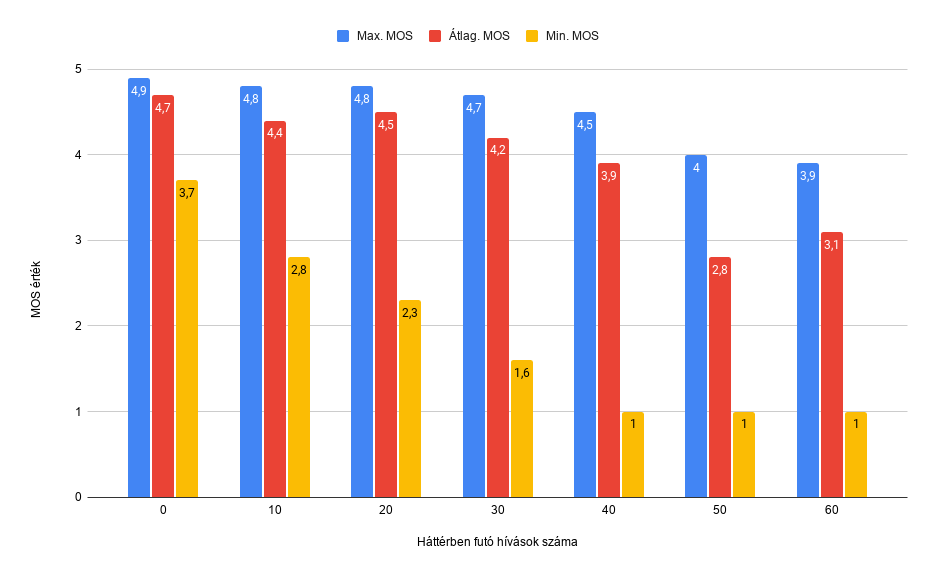
\includegraphics[width=1\textwidth, keepaspectratio]{figures/mos.png}
	\caption{MOS-LQ változása az hívás során adott változó háttérforgalmak mellett.}
	\label{fig:moslq}
\end{figure}

Csak a \texttt{MOS-LQ} alakulása került ábrázolásra, mert a \texttt{MOS-CQ}-val szemben 
csak nagyon kevés különbség van. Látható, hogy adott mennyiségű háttérhívás esetén mennyire romlik a teljes értékű Linphone hívásnak a minősége.

%\begin{figure}[!ht]
%	\centering
%	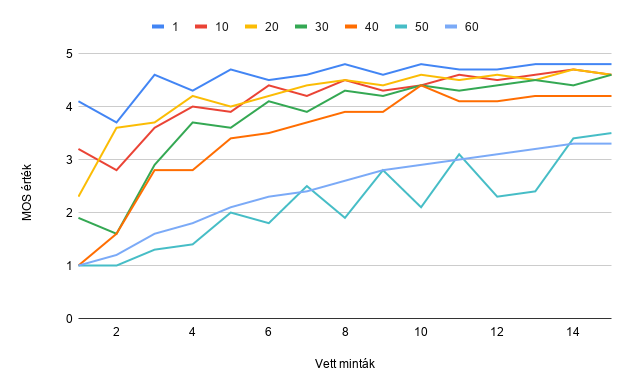
\includegraphics[width=1\textwidth, keepaspectratio]{figures/moscq.png}
%	\caption{MOS-LQ változása az hívás során adott változó háttérforgalmak mellett.}
%	\label{fig:moscq}
%\end{figure}

A \ref{fig:moslq} ábrán látható, hogy a MOS minimális értéke az jóval kisebb minden 
esetben, mint az átlaga. Ez annak köszönhető, hogy a hívás kezdetekor az L7mp proxyk nem 
képesek elég gyorsan feldolgozni a csomagokat így a magas Jitter keletkezik, ami rossz 
irányba befolyásolja a MOS értéket. Ezzel szemben a sokkal jobb átlagos és maximális MOS 
érték annak köszönhető, hogy a Linphone kliens alkalmaz egy adaptív Jitter puffert, 
aminek a méretét annak megfelelően állítja, hogy mekkora Jitter keletkezik a hívás során. 

%Ennek a Jitter puffernek az alakulása látható a 
%A \ref{fig:moslq} ábrán jól látható az folyamat, hogy a hívás kezdte után mennyire rossz 
%a hívás minősége illetve, hogy egy idő után mennyire javul és vesz fel egy viszonylag kis 
%kilengésekkel rendelkező értéket. A hívás elején tapasztalható rossz minőséget az okozza, 
%hogy az okozza, hogy az L7mp proxyk nem képesek elég gyorsan feldolgozni a csomagokat így 
%a magas Jitter keletkezik a rendszerben, amikre nincs felkészülve egyik Linphone kliens 
%sem. Később azért lesz jobb a MOS értéke, mert a kliensek adaptív Jitter pufferel 
%rendelkezni így idővel megtanulják azt, hogy mekkora az átlagos Jitter és annak 
%megfelelően növelik a pufferük méretét, ezzel kisimítva a csomagok érkezését. 

De ez nem jelenti azt, hogy a hívás maradéktalanul jó lesz, amit mutat a
\ref{fig:voiceComp} ábra is, amit a \texttt{WireShark} RTP folyam elemzőjéből mentettem 
ki. 

\begin{figure}[!ht]
	\centering
	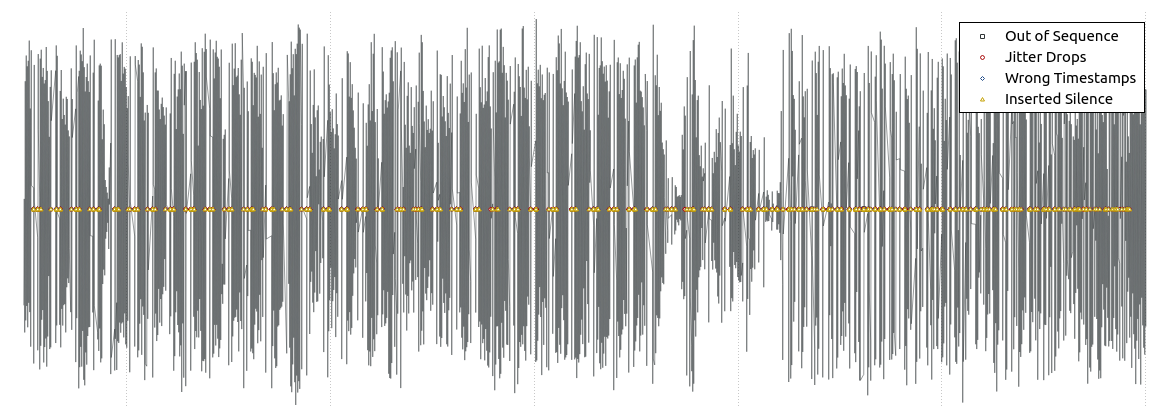
\includegraphics[width=0.7\textwidth, keepaspectratio]{figures/calls60.png}
	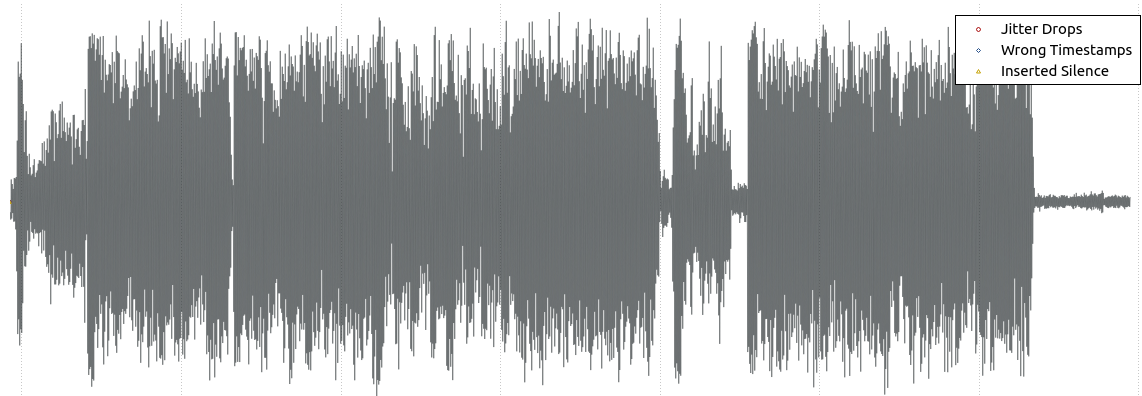
\includegraphics[width=0.7\textwidth, keepaspectratio]{figures/calls20.png}
	\caption{MOS-LQ változása az hívás során adott változó háttérforgalmak mellett.}
	\label{fig:voiceComp}
\end{figure}

A \ref{fig:voiceComp} ábrán a felső hullám 60 hívás mellett készült, míg az alsó 20 hívás 
mellett keletkezett. Ezek azok a RTP folyamok, amik az rtpengine felől érkeztek a 
kliensek felé. 

Jól látszik, hogy a felsőnél rengeteg csend van beszúrva, ami nagyon recsegőssé teszi a 
hívást és élvezhetetlenné, míg az alsónál csak az elején található egyszer egy magas 
Jitter érték, ami nem befolyásolja annyira a hívás minőségét.

\begin{table}[ht]
	\footnotesize
	\centering
	\begin{tabular}{l c c c c c c c}
		\toprule
		 & 0 & 10 & 20 & 30 & 40 & 50 & 60\\
		\midrule
		MOS-LQ & 4,7 & 4,4 & 4,5 & 4,2 & 3,9 & 2,8 & 3,1\\
		MOS-CQ & 4,7 & 4,4 & 4,5 & 4,2 & 3,9 & 2,8 & 2,9\\
		R-Faktor & 94 & 88 & 90 & 84 & 78 & 55 & 59\\
		RTT & 17 ms & 9 ms & 17 ms & 16 ms & 16 ms & 42 ms & 182 ms\\
		Jelszint & -3 & -2 & -4 & -3 & -2 & -8 & -2\\
		Zajszint & -11 & -11 & -12 & -13 & -10 & -22 & -10\\
		Jitter & 2 ms & 7 ms & 13 ms & 5 ms & 66 ms & 69 ms & 173 ms\\
		Max Jitter puffer & 104 ms & 41 ms & 75 ms & 64 ms & 75 ms & 89 ms & 234 ms\\
		\bottomrule
	\end{tabular}
	\caption{Adott háttérhívás mellett mért mutatók átlagai.}
	\label{tab:callValues}
\end{table}

A \ref{tab:callValues} táblázatban jól látszik, hogy a hívások minősége miként romlott 
annak függvényében, hogy hány háttérhívás volt egyszerre. Rögtön észrevehető, hogy a 
MOS értéke az folyamatosan rosszabb attól függetlenül, hogy a \ref{fig:moslq} ábrán az 
látható, hogy idővel javul ennek az értéke. Ez attól van, hogy itt már az összes  
értelmezhető RTCP üzenet fel lett dolgozva és egy idő után beállt a MOS értéke egy adott 
szintre, ezért folyamatos csökkenés látható. 

A másik ilyen könnyen jellemezhető érték azaz R-Faktor, ahol jól látszik, hogy nulla 
háttérhívás mellett átlagosan sikerült elérni azt a minőséget, ami majdnem tökéletesnek 
számít. Ezt a viszonylag jó értéket tartja egészen 40 hívásig, ahol is már egy nagy esés 
látható. Ez már azt jelenti, hogy élvezhetetlen a hívás. Ennek kiváltó oka lehet a magas 
Jitter, ami már ennyivel képes torzítani a hívást. A Jitter egész tolerálható értékeket 
adott 40 hívásig, viszont azután már túl nagyok voltak, mivel 60 ms alatt nagyjából három 
RTP csomagnak kellett volna érkeznie.

A Linphone 60 ms-s Jitter pufferrel rendelkezik alap esetben és, ha szükség van rá, akkor 
ezt képes módosítani. Ez látszik a táblázat utolsó sorában is, mivel adaptívan növeli 
puffer méretet.

\section{Rugalmasság mérése}

A rugalmasság mérése során az fog kiderülni, hogy egy rtpeninge meghibásodása, milyen 
módon befolyásolja a hívást. Ennek szimulálása érdekében a hívás indítása után 
megvizsgálom a Kubernetes fürtben szereplő rtpengine kapszulákat, hogy melyik kezdte 
el feldolgozni a hívást és azt a kapszulát törlöm. Az elvárt működés során annak kell 
történnie, hogy az L7mp operátor képes detektálni a kapszula törlését melynek során 
értesíti az L7mp proxykat, hogy az az rtpengine kapszula már nem elérhető. Ennek hatására 
az L7mp proxykban definiált terheléselosztó egy új végponthoz fogja továbbítani a 
beérkező RTP és RTCP csomagokat. 

A leírt eljárás során nem képesek az RTP és RTCP csomagok eljutni egyik rtpengine 
kapszulához sem, ezért kiesést kell tapasztalni. De ennek a kiesésnek minél rövidebb 
időnek kell lennie, különben a hívásban résztvevő felek nem hallanak bizonyos részeket. 
Ezenfelül okozhat még kapcsolatvesztést is a klienseknél, ha egy adott ideig nem érkezik 
semmilyen médiaforgalom. 

\begin{figure}[!ht]
	\centering
	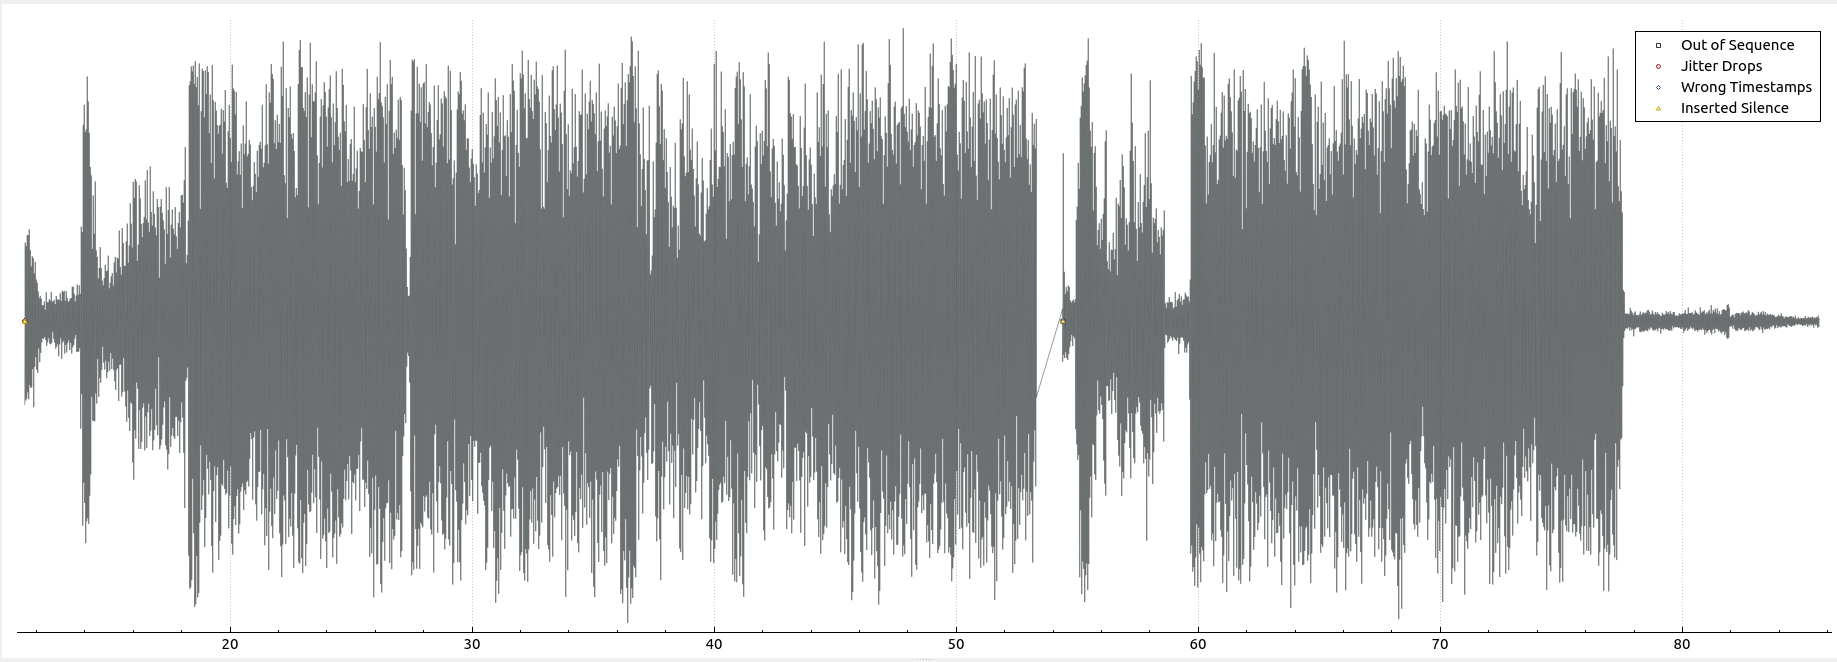
\includegraphics[width=1\textwidth, keepaspectratio]{figures/res.png}
	\caption{Elvesztett beszédrészlet meghibásodás esetén}
	\label{fig:res}
\end{figure}

A \ref{fig:res} ábrán látható, hogy médiafolyam során hol keletkezett kiesés az rtpengine kapszula törlése után. Ez a kiesés összesen 1,1 másodperc kiesést okozott ami a beérkezett csomagok 1,4\% százalékának az elvesztését jelenti.

Összességében elmondható, hogy ezt a feladatot jól ellátja az így létrehozott architektúra, mivel egy ekkora kiesés még nem biztos, hogy kellemetlen lehet a felhasználók számára. Emellett a hívás minősége is megmaradt a törlés után. 
%----------------------------------------------------------------------------   
\chapter{Összefoglalás}
%----------------------------------------------------------------------------

A szakdolgozat megvalósítása során rengeteg új ismerettel lettem gazdagabb, 
amiket tudok majd kamatoztatni későbbi munkáim során. Emellett sikerült 
egy komplex architektúrát megalkotni, amivel Kubernetes alatt lehet 
VoIP hívásokat kezelni. Így sokkal magabiztosabb tudásom lett Kubernetes és 
Python terén is. 

Dr. Rétvári Gáborral terveink között szerepel ennek a projektnek a továbbvitele, 
ami során új funkciókkal kerülne kibővítésre és sokkal nagyobb teljesítményt 
lehetne elérni. 

Terveink között szerepel, hogy az L7mp-t tudjuk a kernel névtérben futtatni vagy 
a szolgáltatáshálóban lecserélni az L7mp-t Envoy-ra, ami sokkal nagyobb teljesítményre
képes. Így valószínűleg sokkal több hívást lehetne párhuzamosan kiszolgálni jelentősebb
minőségbeli romlás nélkül. 

Szeretnénk a kontrollert oly módon megvalósítani, hogy a külvilág számára elérhető
legyen és úgy viselkedjen, mint egy SIP szerver. Így a SIP szerver és az rtpengine 
között sokkal kevesebb komponens lenne, amin keresztül kommunikálni tudnak egymással. 
Ami lehetségesen megoldaná azt a problémát, hogy adott terhelés mellett a Kamailio
már nem tud kommunikálni az rtpengine-l.

Amit még lehet módosítani a rendszeren azaz rtpengine olyan szintű fejlesztése, ami 
lehetővé teszi számunkra azt, hogy Kubernetes kompatibilisen tudjon futni. Ez azt jelenti,
hogy több rtpengine kapszula esetén mindig csak egy kapszula proxyja lenne felkonfigurálva
a híváshoz szükséges szabályokkal. Viszont, ha használt rtpengine kapszula valami miatt 
megszűnik, akkor képes legyen egy olyan értesítést adni valamelyik komponensnek ami 
felkonfigurálja a második rtpengine kapszulát is. \\

Összesítve ez egy nagyon izgalmas téma, amit szívesen folytatnék és fejlesztenék 
a mesterképzés során. 

% Acknowledgements
%~~~~~~~~~~~~~~~~~~~~~~~~~~~~~~~~~~~~~~~~~~~~~~~~~~~~~~~~~~~~~~~~~~~~~~~~~~~~~~~~~~~~~~
%----------------------------------------------------------------------------
\chapter*{\koszonetnyilvanitas}\addcontentsline{toc}{chapter}{\koszonetnyilvanitas}
%----------------------------------------------------------------------------

Ez nem kötelező, akár törölhető is. Ha a szerző szükségét érzi, itt lehet köszönetet nyilvánítani azoknak, akik hozzájárultak munkájukkal ahhoz, hogy a hallgató a szakdolgozatban vagy diplomamunkában leírt feladatokat sikeresen elvégezze. A konzulensnek való köszönetnyilvánítás sem kötelező, a konzulensnek hivatalosan is dolga, hogy a hallgatót konzultálja.


% List of Figures, Tables
%~~~~~~~~~~~~~~~~~~~~~~~~~~~~~~~~~~~~~~~~~~~~~~~~~~~~~~~~~~~~~~~~~~~~~~~~~~~~~~~~~~~~~~
%\listoffigures\addcontentsline{toc}{chapter}{\listfigurename}
%\listoftables\addcontentsline{toc}{chapter}{\listtablename}


% Bibliography
%~~~~~~~~~~~~~~~~~~~~~~~~~~~~~~~~~~~~~~~~~~~~~~~~~~~~~~~~~~~~~~~~~~~~~~~~~~~~~~~~~~~~~~
\addcontentsline{toc}{chapter}{\bibname}
\bibliography{bib/mybib}


% Appendix
%~~~~~~~~~~~~~~~~~~~~~~~~~~~~~~~~~~~~~~~~~~~~~~~~~~~~~~~~~~~~~~~~~~~~~~~~~~~~~~~~~~~~~~
%%----------------------------------------------------------------------------
\appendix
%----------------------------------------------------------------------------
\chapter*{\fuggelek}\addcontentsline{toc}{chapter}{\fuggelek}
\setcounter{chapter}{\appendixnumber}
%\setcounter{equation}{0} % a fofejezet-szamlalo az angol ABC 6. betuje (F) lesz
\numberwithin{equation}{section}
\numberwithin{figure}{section}
\numberwithin{lstlisting}{section}
%\numberwithin{tabular}{section}

%----------------------------------------------------------------------------
\section{A TeXstudio felülete}
%----------------------------------------------------------------------------
\begin{figure}[!ht]
\centering
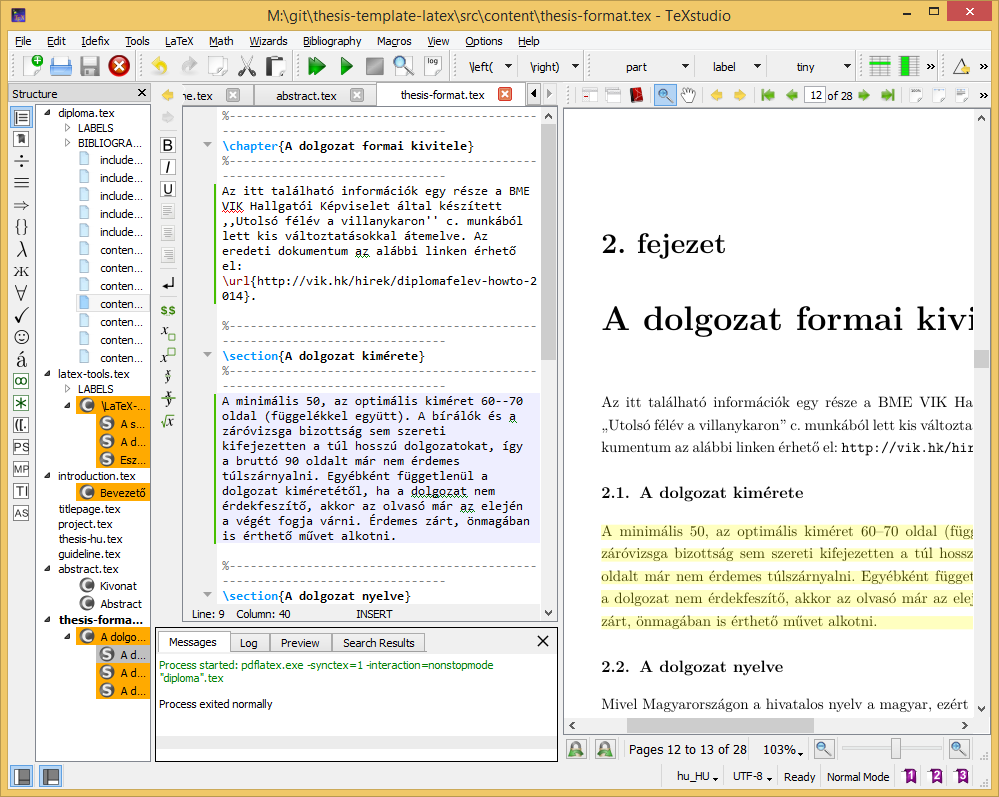
\includegraphics[width=150mm, keepaspectratio]{figures/TeXstudio.png}
\caption{A TeXstudio \LaTeX-szerkesztő.} 
\end{figure}

%----------------------------------------------------------------------------
\clearpage\section{Válasz az ,,Élet, a világmindenség, meg minden'' kérdésére}
%----------------------------------------------------------------------------
A Pitagorasz-tételből levezetve
\begin{align}
c^2=a^2+b^2=42.
\end{align}
A Faraday-indukciós törvényből levezetve
\begin{align}
\rot E=-\frac{dB}{dt}\hspace{1cm}\longrightarrow \hspace{1cm}
U_i=\oint\limits_\mathbf{L}{\mathbf{E}\mathbf{dl}}=-\frac{d}{dt}\int\limits_A{\mathbf{B}\mathbf{da}}=42.
\end{align}


%\label{page:last}
\end{document}
